\documentclass[extern,palatino]{cgMA}

\usepackage{pdfpages}
\usepackage[hyphens]{url}
\usepackage{hyperref}
\usepackage[]{algorithm2e}
\usepackage{caption}
\usepackage{subcaption}
\usepackage{listings}
\usepackage{color}
\usepackage[section]{placeins}
\usepackage{enumitem}
\usepackage{siunitx}
\usepackage{amsmath}
\usepackage{multirow}
\usepackage{changepage}
%\usepackage[export]{adjustbox}

\lstset{
  basicstyle=\ttfamily,
  columns=fullflexible,
  frame=tb,
  captionpos=b,
  breaklines=true,
  postbreak=\mbox{\textcolor{red}{$\hookrightarrow$}\space},
}
\author{Rejnald Lleshi}
\title{Video Based Human Action Recognition Using Deep Learning}
\erstgutachter{Prof. Dr. Ulrich Furbach}
\erstgutachterInfo{Institute for Computer Science}
\zweitgutachter{Dipl.-Inform. Markus Maron}
\zweitgutachterInfo{wizAI Solutions GmbH}
\externLogo{7cm}{logos/west.png}

\begin{document}
\selectlanguage{english}
\maketitle
\newpage
\clearpage
\newpage
\pagenumbering{roman}

\newpage
\section*{Acknowledgments}
\label{acknowledgements}
When writing an acknowledgment for a thesis there are two approaches that one can take: the Indian and the Western one. The former is characterized by a high threshold, which invariably gives more value to the action of thanking someone because it does so only when it is apt to do so. On the contrary, the latter has the threshold so low that the act of thanking is inevitably devalued (the interested reader can further refer to this\footnote{\url{https://medium.com/illumination/the-indian-vs-western-perspective-on-thank-you-27f687cde4fe}} article). Based on the Indian approach, I would like to express my gratitude to 
Prof. Dr. Ulrich Furbach for granting me with the opportunity to work on this thesis and of course, his supervision and valuable feedback, and my colleague at WizAI\footnote{\url{https://wizai.com/}}, Julian Rogawski for his miscellaneous tips along the way. I would also like to thank Markus Maron for granting me the opportunity to work at WizAI in the first place. Finally, I am grateful for having had the opportunity to have worked on my master thesis in the context of an exciting project such as the Vortanz\footnote{\url{https://vortanz.ai/#/de}} project is.

\newpage
\section*{Abstract}
Action recognition is a task that has proven central in gaining insights from videos. It has received growing attention in computer vision and has improved significantly in recent years. Its goal is to identify which human actions appear at which point during a video. Video data is particularly challenging to work within computer vision because it contains complex temporal dynamics due to the variety of actions, speed, or camera motion. This thesis seeks to apply such methods in a dance-like context for didactical purposes. Specific, dance-like movements from the BAST analysis were studied and evaluated with standard and state-of-the-art algorithms from the field. The BAST analysis examines the relationship between movement and inner psychological state and is typically employed in domains such as psychiatry or clinical psychology. However, because BAST utilizes patterns originating from the Laban analysis, a famous movement analysis methodology in dancing, it could be helpful to investigate and try to extend such movements in a dancing context. Different models are trained on BAST material and evaluated in possible dancing contexts to examine their robustness. Various modalities for feature representation, such as RGB frames, optical flows, and human skeletons, were utilized. In order to build high-performance classifiers, and in the absence of a robust training dataset, transfer learning was employed and examined in detail. This work also examined the exact role that the background played towards the models' final predictions.


\newpage
\pagenumbering{arabic}
\tableofcontents
\newpage

\listoffigures
\addcontentsline{toc}{section}{List of Figures}
\newpage

\listoftables
\addcontentsline{toc}{section}{List of Tables}
\newpage

\addcontentsline{toc}{section}{List of Listings}
\lstlistoflistings
\newpage

\section{Introduction}
\label{Introduction}

\subsection{Human Action Recognition in Videos}
\label{intro_har}

Human Action Recognition (HAR) is a field that has emerged very prominently in the last few years. Its applications range from human-robot interaction and video surveillance to education or entertainment, to name but a few \cite{pareek2021survey}. It is a challenging problem compared to still image classification due to the natural diversity and richness that videos inherently contain. The crucial aspect of HAR is temporal relational reasoning, as it forms the building blocks for describing the steps of the action. An activity can consist of several temporal relations at short-term timescales as well as long-term timescales. For example, the activity of \textit{sprinting} contains the long term relations of crouching at its start, running on track in the middle, and finally finishing at the end line, whilst on a shorter-term it contains activities such as periodic hand or feet movement \cite{zhou2018temporal}. To further exacerbate the task, the action under inspection could be the same over various videos, but lightning variations, changes in perspective, different background conditions, or partial occlusions could significantly impact the model’s ability to recognize this same action. HAR models should thus label the same activity with the same label regardless of their subtle subparts or variety. Four broad categories pertain to activity recognition \cite{aggarwal2011human}:

\begin{enumerate}
\item Gesture: Atomic movements of body parts that capture some meaningful motions of a person, e.g., applauding gestures or arm stretching gestures.
\item Action: Complete movements conducted by a person such as \textit{running}, \textit{falling} or \textit{texting}.
\item Interaction: Actions involving two actors, e.g. person-person interactions or person-object interactions.
\item Group Activity: Actions performed by more than two actors, e.g. \textit{having a meeting} or \textit{group dancing}.
\end{enumerate}

The input stream of data representing an action can vary widely from simple RGB or RGB-depth to pose or sensor data, with each of them presenting its unique challenges. The main aim of this thesis is to study the performance and recognition accuracy of single-person actions in videos. Hence the other types of activity recognition such as interaction and input streams such as sensor data are not explored. 

A video is a sequence of images called frames. Hence, while frames are static and capture the spatial components, it is the temporal component of videos that captures the dynamic evolution of an event. In RGB videos, each image frame is a three-dimensional grid of pixels, where each dimension represents the intensity of Red (R), Green (G), and Blue (B) colors, respectively. The values are 8-bit numbers ranging from 0 – 255, with higher numbers representing higher intensities. This means that in total, a single frame can take up to $256^{3}$ different colors. 

\begin{figure}[h]
\center
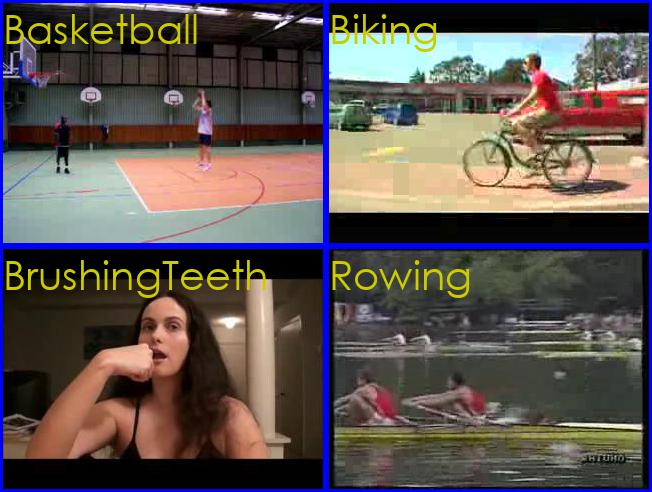
\includegraphics[height={170pt}]{images/ucf_actions.jpg}
\caption{Four actions from the Ucf101 dataset on human action recognition}
\label{ufc_actions}
\end{figure}

The goal of HAR is to map a particular action to a frame that describes an instance of that action. Figure \ref{ufc_actions} shows four such examples from the Ufc dataset \cite{soomro2012ucf101}. In the first example, the current frame describes a person playing basketball, and we would like the model to associate such a frame with the label \textit{basketball}. Hence, Human Action Recognition aims to label human activities, i.e., label the movements of one or several parts of the human body. HAR models must utilize information across the video to capture its richness and the developing action to come up with the correct prediction for the individual frames.

Generally speaking, the models used for HAR are divided into two broad categories: conventional, handcrafted-feature based machine learning techniques such as Support Vector Machine, Nearest Neighbor, Hidden Markov Model, and Random Forest \cite{pareek2021survey} and deep learning techniques such as Convolutional Neural Network or Recurrent Neural Network.
The focus of this thesis has been studying Deep Convolutional Neural Networks to perform HAR on the specific domain of Motion Analysis Scales and Test \cite{lausberg1997bewegungsdiagnosetest}.

\subsection{Motion Analysis Scales and Test (BAST)}
\label{intro_bast_laban}

"Bewegungs Analyse Skalen und Test" (BAST), here rendered in English as Motion Analysis Scales and Test (but still abbreviated as BAST in this work for the sake of clarity), is an analysis system designed for expressive body movements \cite{lausberg1997bewegungsdiagnosetest}. Its focus is the analysis of casual movements such as running or stamping but even more complex dance-like movements. The examination consists of a movement diagnostic test followed by an evaluation of these movements and questionaries for self-assessment of movement behavior which last about 10 minutes and are given verbally by a test administrator\footnote{Bast Website --- \url{https://bast.neuroges-bast.info/en}}. Originally, BAST was designed to investigate the relation of body movements to specific mental functions, which is why it has been frequently applied for diagnostic purposes in psychiatry, psychosomatic medicine, and clinical psychology\footnote{Bast Research --- \url{https://bast.neuroges-bast.info/research-projects}}.

The BAST analysis traces its roots to the Laban Movement Analysis (LMA). LMA seeks to provide an objective description of movements on different levels by considering them a psycho-physical process and an outward expression of inner intent \cite{groff1995laban}. Originally based on the work of Rudolf von Laban, it has since been expanded and is used today in broad fields ranging from dancing and acting to health professionals. The latter is the case with the BAST analysis. LMA considers four broad categories \cite{groff1995laban}:

\begin{enumerate}
\item Body: distinguishes the individual body parts, their relationships within the body, and what the body is doing.
\item Effort: evaluates the quality of movements in terms of weight, space, time, and flow.
\item Shape: how the body shapes itself in space such as curved, angular, symmetric, or asymmetric.
\item Space: where the body is moving, the direction, location and it’s relationships with the space around it.
\end{enumerate}

\noindent The BAST analysis is based on LMA and has nine base categories: \textit{walk}, \textit{run}, \textit{jump}, \textit{stamp}, \textit{contract-expand}, \textit{tiptoe}, \textit{swing upper body}, \textit{rotate} and \textit{fall}. These categories are then evaluated based on the four broad categories of LMA presented above, more specifically, on dimensions such as the performance, floor contact, kinesphere, floor pattern, space dimension, etc. as described in details in the Section \ref{background_bast}. For instance, the \textit{walk} movement could be evaluated based on its floor pattern into four categories \cite{lausberg1994vergleichende}:

\begin{enumerate}
\item walk straight: The floor pattern is (almost) only straight and is (almost) not curved.
\item walk rather straight: The floor pattern is straight and curved but mostly straight.
\item walk rather curved: The floor pattern is curved and straight but mostly curved
\item walk curved: The floor pattern is (almost) only curved (circles, waves) and is (almost) not straight.
\end{enumerate}

\subsection{Problem Statement and Motivation}  
\label{problem_statement_and_motivation}

Based on the LMA analysis, the BAST analysis could have applications outside the psychological context, as mentioned previously. We will investigate such applications in the context of the \textit{Vortanz}\footnote{Official Website --- \url{https://vortanz.ai/}} project, where we seek to integrate machine learning methods to university level dance education in an insightful way. Such A.I. algorithms will be used for didactical purposes in various universities in Cologne, Frankfurt, and Berlin. It is in the context of this project that this thesis has been developed. One possibility is to investigate how well A.I. models can recognize complex, dance-like movements from BAST and if such movements could be extended to other, dance-like contexts. This could potentially open up possibilities for different didactical use-cases further along the duration of the project. More specifically, this thesis investigates the movements presented in Section \ref{background_bast} of the BAST analysis as well as their corresponding evaluations.

\bigskip
\noindent\textbf{The first aim of this work is to build robust A.I. models that recognize the nine basic movements and their evaluations and then to investigate how well they might generalize in other dance-like contexts.}

\bigskip

\noindent \textbf{The second aim of this thesis is to investigate the role of background in the final predictions of the trained HAR models as well as the role of transfer learning from benchmark datasets in the field of HAR in the BAST domain.}

\subsection{Research Objectives and Research Questions}
\label{research_objectives_and_research_questions}

The primary objective of this thesis is to leverage deep learning to classify movements and their evaluation from the BAST analysis. The focus is to evaluate how good state-of-the-art models can recognize such complex human activities and investigate how robust they are, i.e., how well they generalize for other contexts, specifically, dancing contexts. The research questions in the scope of this thesis are as follows:
\bigskip \bigskip \bigskip

\emph{Research Question 1:}
\bigskip
\begin{adjustwidth}{100}{0}
Which is the best Human Action Recognition (HAR) model for classifying the nine base movements (\textit{walk}, \textit{run}, \textit{jump}, \textit{stamp}, \textit{contract/expand}, \textit{swing upper body}, \textit{rotate}, \textit{fall}) of the BAST analysis?
    
\bigskip
\noindent The goal here is to train different models and find the one that has the highest \textit{top-k} accuracy. For the base annotations, the aim is to build models that can generalize in other domains.

\noindent Research question 1 is answered in Section \ref{research_question_1}.
\end{adjustwidth}

\bigskip \bigskip
\emph{Research Question 2:}
\bigskip
\begin{adjustwidth}{100}{0}
Which is the best Human Action Recognition model for classifying the evaluation of the nine base movements of the BAST analysis?
\bigskip

\noindent The evaluation of the movements of the BAST analysis poses quite complex use cases. For example, we need to evaluate whether \textit{stamping} is done with little strength or maximum strength or to what extend the head has been integrated into the movement. Demonstrating that deep HAR models can learn such subtle evaluations could be useful for other contexts. The question, whether the BAST evaluation process in itself can be automatized is also investigated.

\noindent Research question 2 is answered in Section \ref{research_question_2}.
\end{adjustwidth}

\bigskip \bigskip
\emph{Research Question 3:}
\bigskip
\begin{adjustwidth}{100}{0}
How robust are the models trained in a BAST context? 
\bigskip

\noindent After training models with the provided datasets their robustness to generalize to other domains is tested. Two domain tests are specifically carried out. The first one investigates whether the nine base categories of BAST can be used as general representative categories in a dance-like context. The second one examines if the \textit{kinesphere} evaluation of BAST can be extended, that is recognized, in a dancing context.

\noindent Research question 3 is answered in Section \ref{research_question_3}. The first experiment in Section \ref{research_question_3_1} and the second one in Section \ref{research_question_3_2}.
\end{adjustwidth}

\bigskip \bigskip
\emph{Research Question 4:}
\bigskip
\begin{adjustwidth}{100}{0}
How important is transfer learning for the models' performance?
\bigskip

\noindent Generally speaking, image recognition models improve if they are first pre-trained on other datasets. This has also been established for HAR models \cite{carreira2017quo}, \cite{duan2020omni}. Nevertheless, does this hold for such corner-cases as the BAST analysis, whose actions have little in common with typical benchmarks in the field of HAR? Moreover, which benchmark dataset in the field of HAR is best suited for this purpose?

\noindent Four experiments were performed for this research question. The first one examined the differences between training the models from scratch and using transfer learning. Next, the differences between using various benchmark datasets for the same task and model architecture were examined. The aim was to find the best-suited benchmark dataset for transfer learning. Thirdly, the benefits of training with the base annotations task for the evaluation annotations were examined; in particular, it was examined whether such pre-training solves the imbalanced-classes problem of the evaluation dataset.

\noindent Research question 4 is answered in Section \ref{research_question_4}.
\end{adjustwidth}

\bigskip \bigskip
\emph{Research Question 5:}
\bigskip
\begin{adjustwidth}{100}{0}
What role does the background play in the model's performance? 
\bigskip

\noindent HAR models are heavily influenced by factors such as the background and lightning variation, occlusions etc. Four experiments were performed to investigate this influence. First of all, the general influence of background variations was shown for HAR models in general terms. Then, this influence was investigated for the models that were trained in this work. Next, the background was stripped, and a background-free dataset was created to train models on it and observe differences with models trained on videos with backgrounds. Finally, skeleton-models are also considered and compared with the previous background-free and standard approach.

\noindent Research question 5 is answered in Section \ref{research_question_5}. Each experiment is investigated from Sections \ref{research_question_5_1} to \ref{research_question_5_4} respectively.
\end{adjustwidth}
\bigskip \bigskip
 
\subsection{Contributions}
\label{contributions}

This work studies the literature of state-of-the-art human action recognition (HAR) models over the last four years and implements such architectures in the context of the BAST domain. To my awareness, this is the first study of this kind. The research that this work is concerned with could be divided into two major avenues. The first aim is to build powerful and robust classifiers on the two tasks of the BAST analysis: the nine basic movements and the evaluation of these basic movements. The second aim is to investigate common nuisances in HAR, such as background variations and lightning occlusions, as well as to investigate the influence of transfer learning in HAR models in the given BAST context.

\bigskip
\noindent On the first front, robust classifiers were build on the nine basic movements of the BAST analysis. The purpose was to study whether they could be extrapolated as major dancing categories in the context of the \textit{Vortanz} project. In other words, movements such as \textit{tiptoe} or \textit{swing-upper-body}, that were originally learned on BAST material, could be picked up in a dancing context as well. In the absence of such datasets where the models trained on the BAST base annotations could be evaluated, this work utilized the second task of the BAST analysis for this purpose. The results are examined in Section \ref{research_question_3}. For the evaluation movements, on the other hand, apart from testing if HAR models are able to pick up such fine-grained movements, the main focus is to investigate if the evaluation process of the BAST analysis in itself could be automated. The end result would be that such models would assist trained examiners of the BAST analysis or replace them altogether.

\bigskip
\noindent The second major avenue of research in this work is to investigate the influence of the background in the tasks at hand and the benefits of using transfer learning. Background influences and lighting variations have been shown to impact the performance of HAR models. Ideally, we would want our models to focus only on the action at hand. If such models are moreover deployed in production,  they must be robust regarding different background appearances. Indeed, it is to be expected that the material uploaded by the students for inspection will contain many different types of backgrounds.  After this influence is investigated, attempts at demeaning it are made by stripping the background or using models that work on a new type of input stream, namely pose. This is further investigated in Section \ref{research_question_5}.

\bigskip
\noindent Transfer learning has been known to tremendously help in various computer vision tasks since the last decade. In the context of this thesis, it became an indispensable instrument to train robust models because the dataset under disposal was small. Hence, in this work, various benchmarks in the field of HAR were examined and compared. Moreover, the BAST analysis presents a very corner use case. Hence one of the questions posed here was whether transfer learning would still be helpful in the domain under inspection. This thesis shows that this is indeed the case and transfer tremendously helps the performance of models trained on BAST material.

\subsection{Thesis Outline}
\label{thesis_outline}

This section outlines the chapters of this thesis and how they are connected. This thesis consists of seven chapters, including the current introduction. Chapter \ref{background} explains the background information of this thesis, namely the theory behind BAST as well as deep learning and convolutional networks. In particular, it explains 2D and 3D Convolutional networks in detail, which were the most common deep learning algorithm used to answer the research questions in this work. Chapter \ref{literature_review} gives an overview of the state-of-the-art human action recognition architectures that were utilized in the context of this thesis. Chapter \ref{experimental_setup} describes the experimental setup of the thesis. It discusses the datasets that were used, the different input modalities, utilized benchmarks for transfer learning, the complete deep learning pipeline, and the evaluation criteria used for the models. 

Chapter \ref{initial_analysis} describes the initial analysis and a few experiments run on the BAST dataset before any of the experiments of the research questions were started. It focuses on the two major problems of the dataset, namely insufficient data and imbalanced classes, and theorizes on possible ways to solve them that will be tested through experiments. Chapter \ref{experiments} describes all the experiments that were conducted in the context of this work and that answer the research questions posed in Section \ref{research_objectives_and_research_questions}. There is a dedicated section for each research question. Finally, Chapter \ref{threats_and_conclusion} highlights the conclusion, limitations and future research possibilities.

\newpage

\section{Background}
\label{background}
This chapter explains the fundamental background that was used to conduct this research. First, a very detailed description of the actions of the BAST analysis is given in section \ref{background_bast}. The two main datasets used for conducting this research are extracted based on that information. Section \ref{background_optical_flow} gives the necessary background to understand the optical flow input modality. The next two Sections, \ref{artificial_neural_networks_background} and \ref{convolutional_neural_networks_background} explain the fundamental theory behind neural networks and convolutional neural networks respectively. Finally, Section \ref{background_skeleton_based_ar} concludes the background information by introducing the use of pose information for human action recognition.

\subsection{BAST}
\label{background_bast}
As already mentioned in the introduction to BAST at Section \ref{intro_bast_laban}, the analysis consists of two parts. Initially, the movement diagnostic test is performed. These movements are thereafter certified by trained professionals. Each movement is performed for about 30 seconds by the subjects. In the second part of the test, four improvisation tasks are given, where the users are asked to emulate \textit{fire}, \textit{earth}, \textit{water} and \textit{air} with their body movements. These movements are also certified by trained professionals. The dataset available for this thesis consisted only of the first part of the test; hence the focus on model training are the annotations from this part. The videos of the second part are missing annotations and can therefore not be utilized for model training. However, they can be used to a certain extent to evaluate the nine fundamental movements since they can represent movements with a different domain and with a generalized context.

\begin{figure}[h]
\center
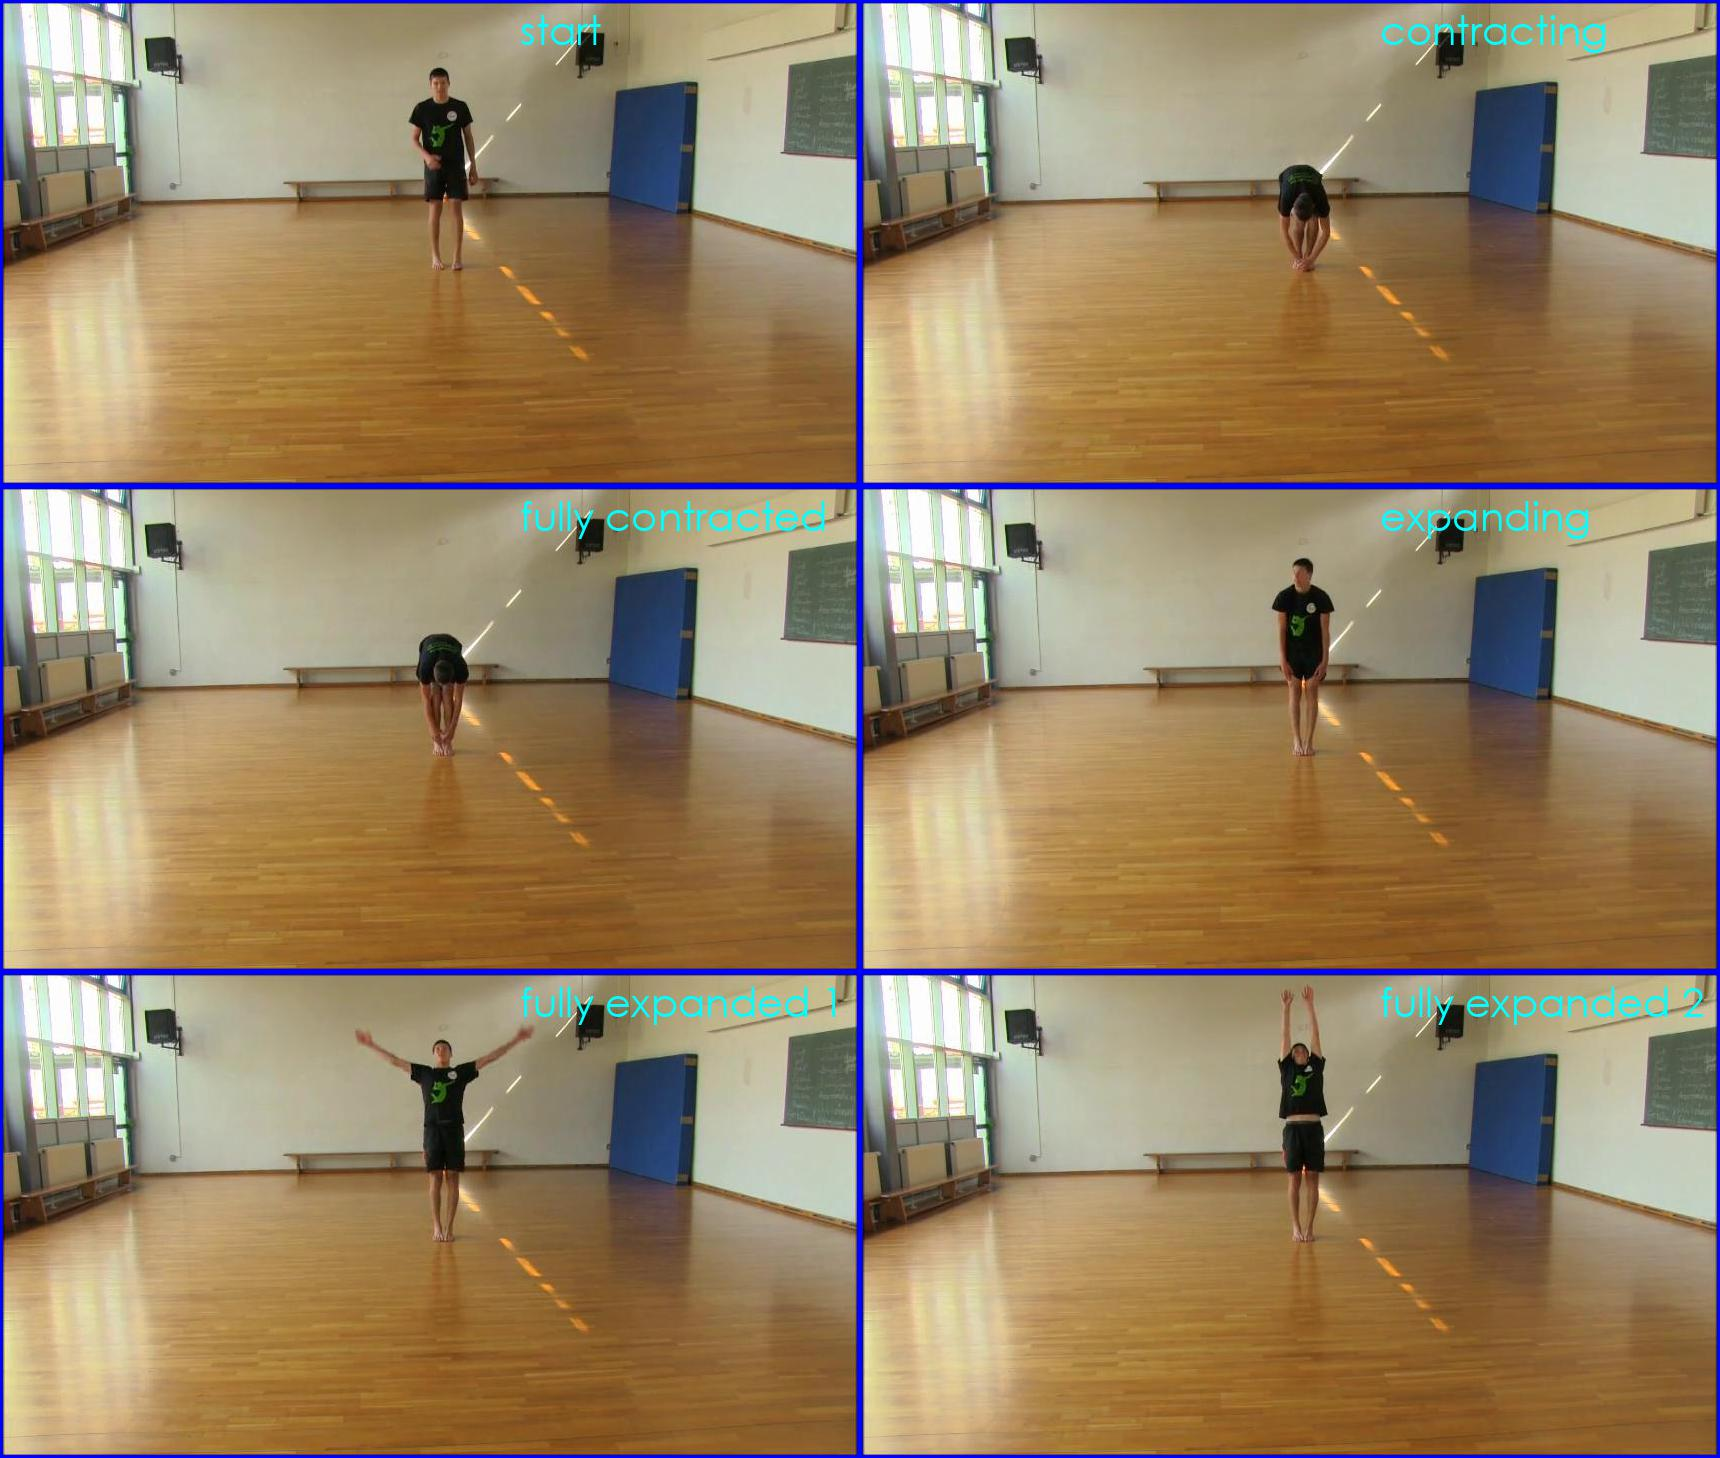
\includegraphics[height={350pt}, width={400pt}]{images/bast_contract_expand.jpg}
\caption{The \textit{contract-expand} movement from the BAST dataset}
\label{bast_contract_expand}
\end{figure}

The nine movements, along with their evaluations, which are the focus of this thesis, are listed below (some of the evaluations have been omitted due to lack of sufficient data. For more details see Section \ref{bast_data}) \cite{lausberg1994vergleichende}:

\begin{enumerate}[I]
\item \textbf{Walking and Running}

    \textbf{Floor pattern:} Patterns that develop as traces of imagined locomotion on the floor. It covers the whole period for the task \textit{walking/running}. Meaning that if evaluated to \textit{curved} the person walks in a curved manner (e.g., circles, waves) during the whole 30-second duration of the task.
    \begin{enumerate}
        \item \textbf{rather straight:} The floor pattern is straight and curved but mostly straight.
        \item \textbf{rather curved:} The floor pattern is curved and straight but mostly curved.
        \item \textbf{curved:} The floor pattern is (almost) only curved and is (almost) not straight.
    \end{enumerate}
\item \textbf{Jumping}

    \textbf{Emphasis:} The emphasis of the jump direction. Which is the participant’s dominant direction during this task? The participants can have more than one direction, but only the dominant one during the duration of the task counts.
    \begin{enumerate}
        \item \textbf{upwards:} The jump aims high up in the air.
        \item \textbf{forward:} The jump aims widely forward.
    \end{enumerate}
    \textbf{Time in air:} Period of time in the air, that is with no floor contact. This is evaluated relative to the participant's physical capabilities.
    \begin{enumerate}
        \item \textbf{long:} There is no floor contact for a rather long period of time. Given his physical capabilities, the participant is not expected to be in the air longer.
        \item \textbf{short:} There is no floor contact for a rather short period of time. Given his physical capabilities, the participant could be in the air longer.
    \end{enumerate}
\item \textbf{Stamping}

    \textbf{Body involvement:} How much is the body utilized in the stamp movement? It is sufficient that the participant shows body involvement only at one moment during the 30-second task.
    \begin{enumerate}
        \item \textbf{isolated:} Only the legs are used for the task. While the rest of the body might still slightly move, it does not really contribute to the power with which the floor is hit.
        \item \textbf{whole body:} The whole body is utilized in the task. 
    \end{enumerate}
    \textbf{Strength:} The amount of strength with which the foot hits the floor. The quality of the highest use of power during the task duration counts and not the average.
    \begin{enumerate}
        \item \textbf{no strength:} During the complete 30-second task, no strength is used when the foot hits the floor. The stamping resembles more like walking or marching.
        \item \textbf{little strength:} Little strength is used when the foot hits the floor.
        \item \textbf{medium strength:} A medium use of power is observed when the foot hits the floor. However, the person could still use more power.
    \end{enumerate}
\item \textbf{Contract-Expand} as shown in Figure \ref{bast_contract_expand}
    
    \textbf{Kinesphere}: A body occupies a particular space at all times. The space that is within personal reach of the body, without it having to move, is defined as the Kine-sphere \cite{block1998keep}. In other words, the kine-sphere consists of the space that is reachable by extending one's limbs.
    Which part of the kine-sphere is reached while performing this task?
    \begin{enumerate}
        \item \textbf{narrow:} During movement, the arms touch the body, and the legs are closed.
        \item \textbf{narrow-medium:} The arms are near the body but do not touch it, and the feet stand hip-width apart. 
        \item \textbf{medium-wide:} The arms are at a small distance from the body, and the legs/feet stand more than hip-width apart. 
        \item \textbf{wide:} The arms/legs are stretched out and (nearly) reach the limits of kine-sphere.
    \end{enumerate}
    
    \textbf{Emphasis:} Whether the emphasis is on contract or expand. Evaluated by checking which is performed for a longer period of time. 
    \begin{enumerate}
        \item \textbf{contracting:} The contracting phase lasts longer.
        \item \textbf{expanding:} The expanding phase lasts longer.
        \item \textbf{no emphasis:} Both phases are roughly equal.
    \end{enumerate}
\item \textbf{Tiptoe}
    
    \textbf{Balance:} Relation between body focus and body basis. Evaluated for the entire time of the task. 
    \begin{enumerate}
        \item \textbf{unstable:} The body focus is not on the body basis. When standing on both feet toes the person touches the ground with the heels or skips (shift of basis).
        \item \textbf{rather stable:} The balance is rather stable.
        \item \textbf{stable:} The body focus is on the body basis. The person is able to stand 15 seconds on both feet toes and 10 seconds on one foot toes without skipping or touching the ground with the heel.
    \end{enumerate}
\item \textbf{Swinging}
    
    \textbf{Flow:} Permanent control vs partial release of the body. The way how the agonistic and antagonistic muscles in back and forth swinging are used. This evaluation specifically targets the part of the body that was swinging, e.g. trunk and/or arms.
    \begin{enumerate}
        \item \textbf{very bound}: The antagonistic muscles counteract the agonistic muscles. The movements are firm, controlled, rather sticky and tense.
        \item \textbf{bound}: The movement is more bound
        \item \textbf{free}: The movement is more free
        \item \textbf{very free}: The agonistic muscles are activated, the antagonistic muscles are relaxed. The movements are flowing free.
    \end{enumerate}
\item \textbf{Spinning}
    
    \textbf{Flow:} "bound", "rather bound", "rather free", "free"
    
    \textbf{Continuity:} How is the spinning performed? Refers to the whole duration of the task.
    \begin{enumerate}
        \item \textbf{single:} The subjects performs only single turns and stop after each turn.
        \item \textbf{discontinued:} Many turns are performed subsequently (\textit{<10}). The turning stops briefly before it starts again.
        \item \textbf{continued:} Continuous turning, i.e. at least 10 turns in succession without stopping.
    \end{enumerate}
    
    \textbf{Acceleration:} The acceleration of the movement. Refers to the whole duration of the task.
    \begin{enumerate}
        \item \textbf{no acceleration:} The speed of spinning is constant or decreasing.
        \item \textbf{acceleration:} The speed of spinning tends to increase. One occurrence is enough.
    \end{enumerate}
\item \textbf{Falling}
     
    \textbf{Flow:} The flow of the movement when falling. Refers to the whole duration.
    \begin{enumerate}
        \item \textbf{lying down:} The flow of the movement is bound. The subject lies or sits down.
        \item \textbf{free:} The falling is a flowing movement of short duration.
    \end{enumerate}
    
    \textbf{End position:} Level on which the falling ends.
    \begin{enumerate}
        \item \textbf{sitting:} The falling ends with sitting, kneeling on all fours.
        \item \textbf{lying:} The falling ends with lying on the floor.
    \end{enumerate}
\end{enumerate}

\subsection{Optical Flow}
\label{background_optical_flow}
A video can be thought of as consisting of two components: a spatial and a temporal component. The spatial component would be the individual frames, which carry information about the objects and scenes depicted. The temporal component can then be thought of as depicting the change/motion across these frames, both from the point of view of the camera as well as the point of view of the objects of the frame. Optical Flow (OF) is a handcrafted feature that can be used to understand how objects are moving in an image at a pixel level. While OF has had many applications in different fields, in human action recognition, it has been used in classical studies that capture changes in the temporal component of a video with methods such as histograms of flow \cite{laptev2008learning}, motion boundary histograms \cite{dalal2006human}, and trajectories \cite{wang2013action}. Moreover, optical flows have also been exploited in the context of deep neural networks. \cite{simonyan2014two} was one of the first to devise a two-stream Convolutional Neural Network, with one stream performing image recognition from static frames and the other utilizing information from stacked optical flows between several consecutive frames before fusing the streams together to get the final result.

The Optical Flow is estimated by calculating each pixel's motion velocity and direction between two successive frames caused by an object or camera movement. Thus OF defines both the orientation as well as the velocity of motion. Below in Figure \ref{flow_swing_figure} the \textit{tvl1} optical flow \cite{perez2013tv} is shown for the \textit{swing upper body} task of the BAST analysis. As expected, the person's movement causes him to be picked up by the optical flow algorithm while the rest of the image appears uniform. In the context of this work, the \textit{tvl1} was the preferred method of extracting the optical flow that was used. Specifically, the optical flow was used in the I3D algorithm.

\begin{figure}[h]
\center
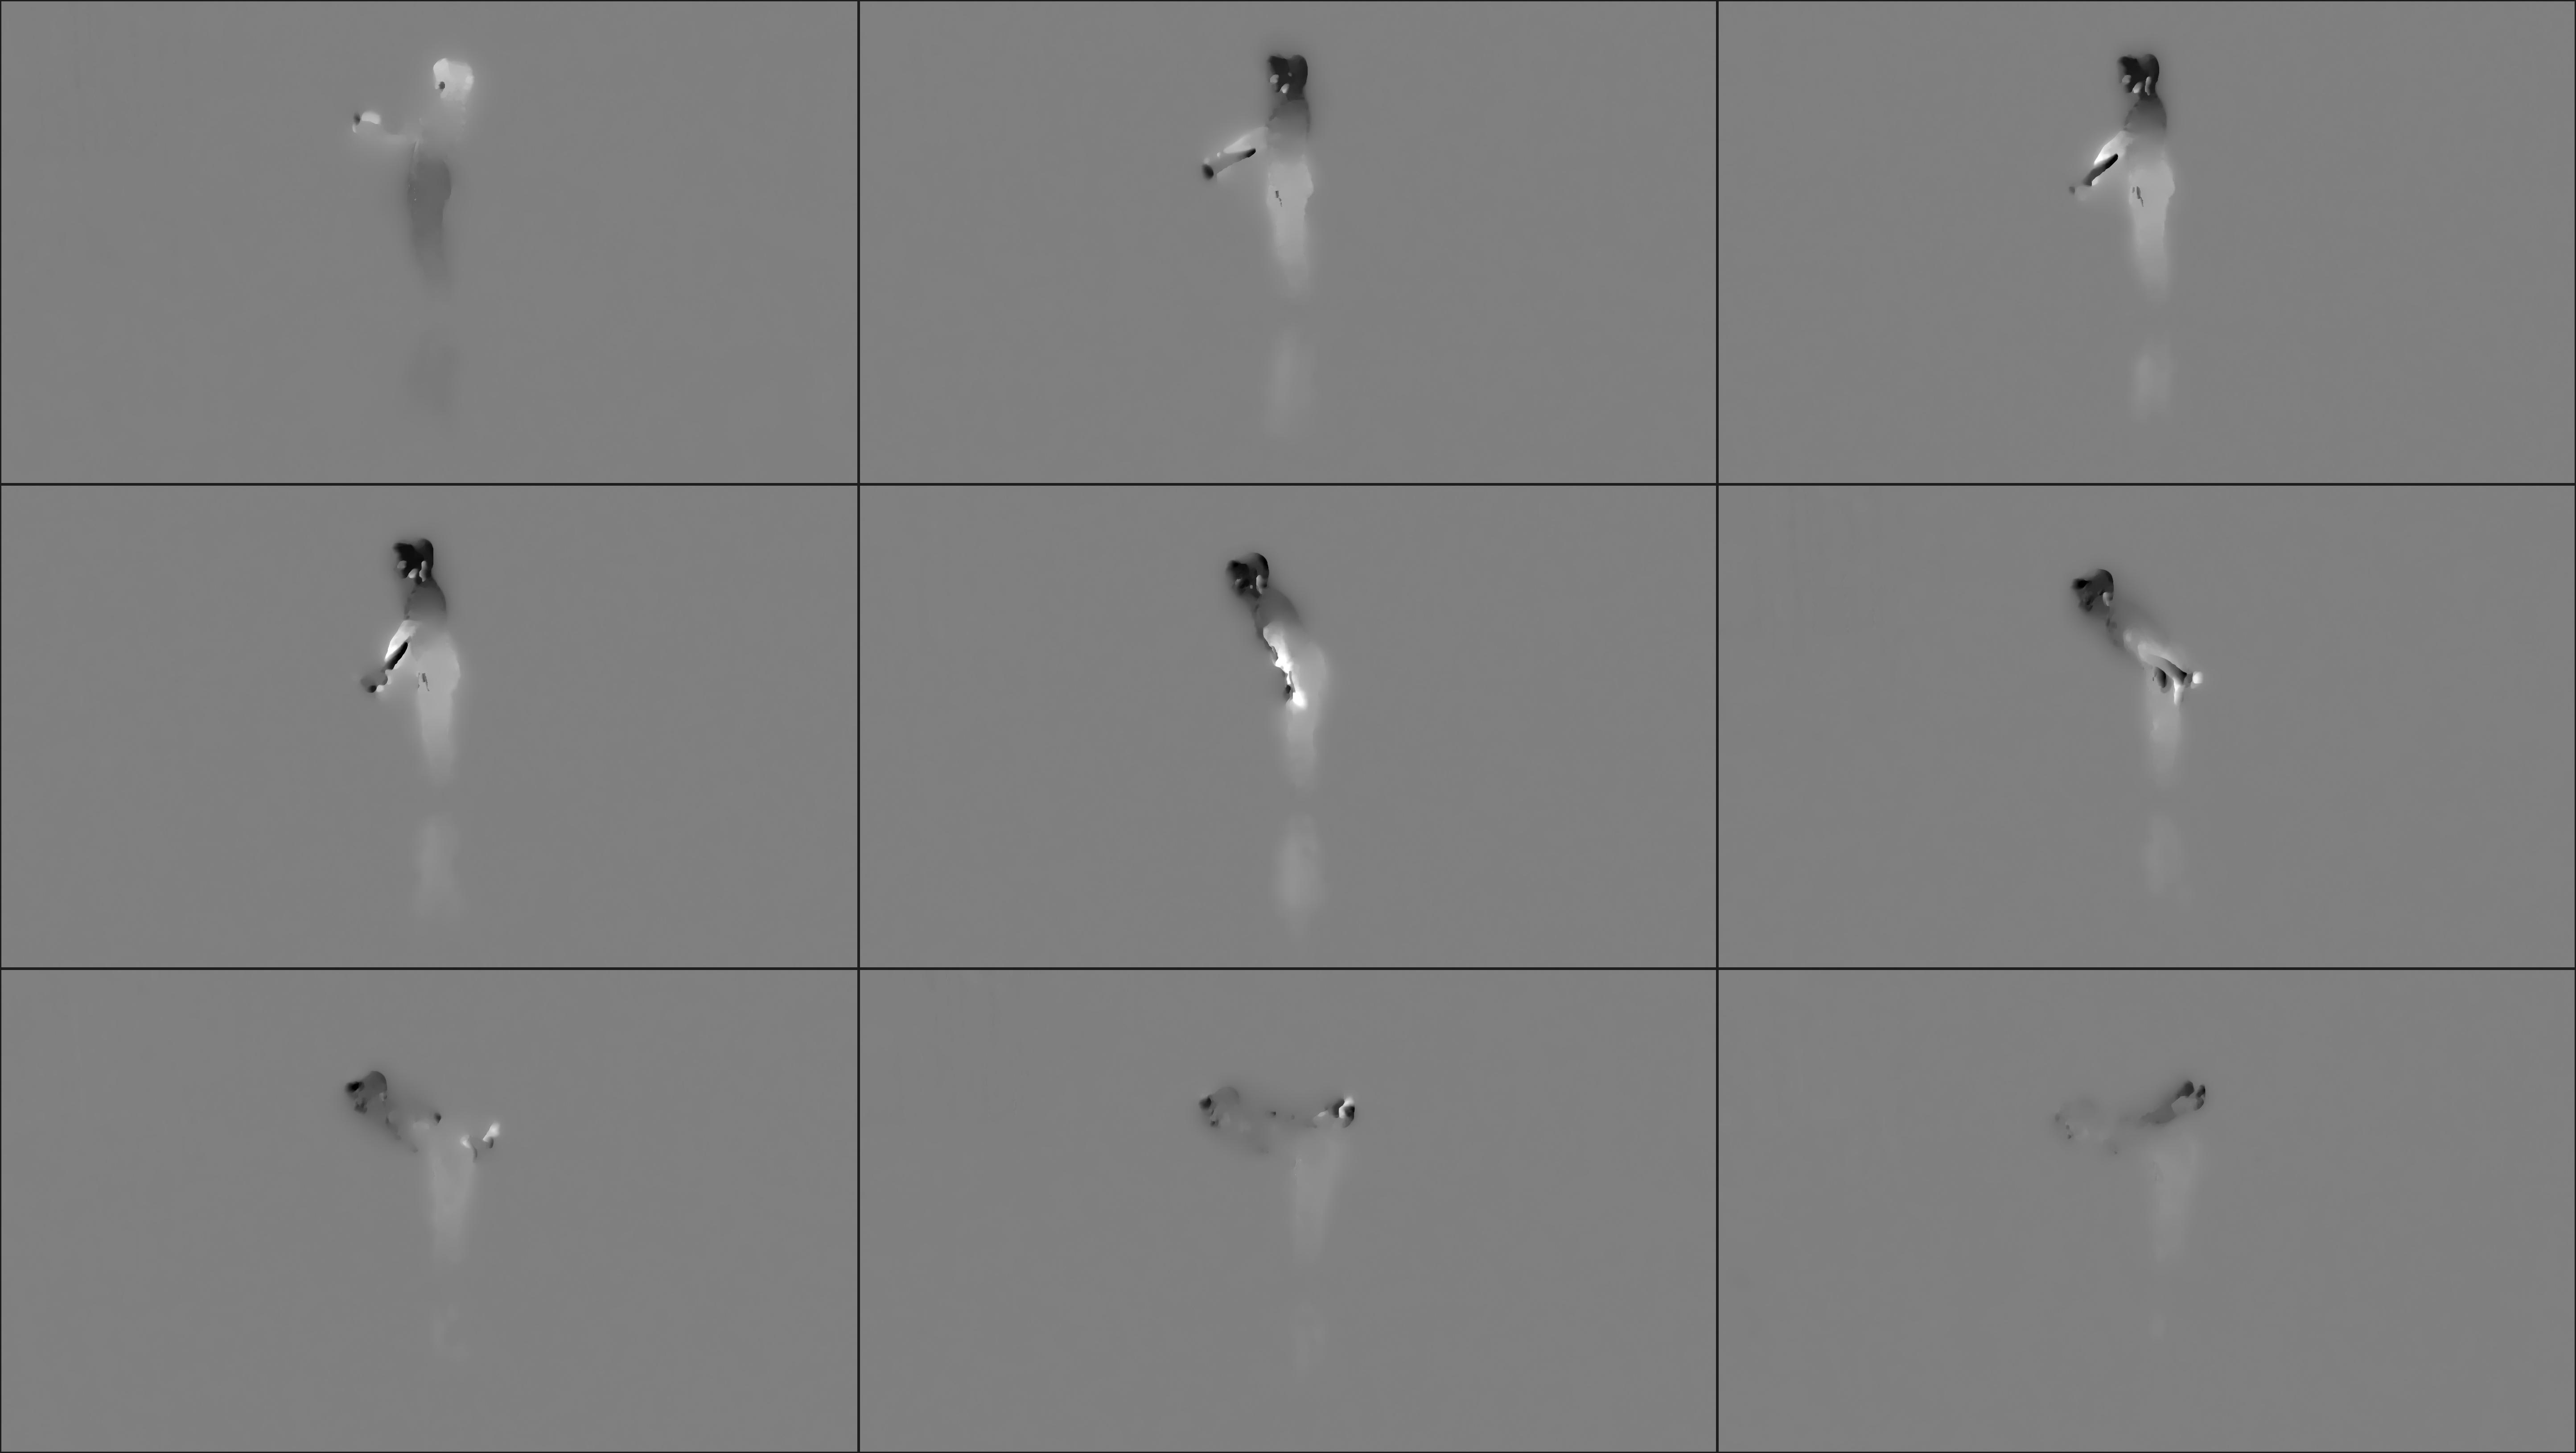
\includegraphics[height={300pt}, width={420pt}]{images/flow_swing.jpg}
\caption{Optical Flow for the \textit{swing upper body task of BAST}}
\label{flow_swing_figure}
\end{figure}


\subsection{Artificial Neural Networks}
\label{artificial_neural_networks_background}

An artificial neural network (ANN) is a system of connected nodes (neurons) that transfer information. It is a mathematical or computational model designed to emulate the human brain, specifically the nervous system. The neuron in itself can be simply thought of as a programming function that takes certain inputs, mathematically manipulates them in some way and then yields one or more outputs. An ANN consists of many such neurons that are interconnected with each other and organized into various layers. This enables it to perform high-level abstractions of the raw data using hierarchical structures, thus avoiding the need for expert knowledge for manual feature extraction, as might be the case with more conventional machine learning methods such as random forests or support vector machines. The deeper a network is, i.e., the more layers it has, the more complex patterns it is able to pick up. What typically happens inside a neuron is a sum of weights, addition of bias, and then finally a squashing of the result in order to insert non-linearity into the neural network and enable learning \cite{nielsen2015neural}. During training, the weights of each neuron are tuned such that a desired output is generated when presented with a particular input. The challenge is to find the proper set parameters so that the model neither underfits nor overfits the training set\footnote{overfitting vs. underfitting --- \url{http://www.pstu.ac.bd/files/materials/1566949131.pdf}}. For example, if the network is too deep, i.e., it has too many hidden layers, the model can overfit the training set. On the other hand, if it is too shallow, the model might underfit the data and not learn anything. 

Figure \ref{ann_mathematical_model} depicts the mathematical model of an ANN. Given an input vector $X_1, ...., X_n$, each value $X_i$ is multiplied by its corresponding weight $W_i$ and then summed up. After a bias $W_0$ is added, an activation function $f$ is applied, which yields the final output $y$. The ANN aim to is to tune the set of weights $W$ of the network that minimizes the amount of the total sum of squared errors, which is computed by the difference between the network's output and the desired (ground-truth) output of the training set. 

\subsubsection{Multi-Layer Perceptron} 

The Multi-Layer Perceptron (MLP) is one of the most popular types of ANNs. It is a feed-forward neural network that consists of multiple layers with neurons that have weighted connections, where each neuron is connected to all the neurons of the next layer \cite{noriega2005multilayer}. The input gets feed-forward through the hidden layers of the network, and the weights of each neuron are modified in order to reduce the sum of squared error as much as possible.  This is typically achieved by using a back-propagation algorithm. An MLP consists of an input layer of neurons, an arbitrary number of hidden layers, and an output layer, which performs the final classification as shown in Fig \ref{multi_layer_perceptron}. Typically the output layer will have as many neurons as the classification task at hand. The idea is that the output node (neuron) that contains the highest activation represents the final classified label \cite{ramchoun2016multilayer}. 

As shown in Figure \ref{ann_mathematical_model}, each neuron has multiple inputs (the outputs of the neurons of the previous layer) and produces an output, which is then fed to the multiple neurons of the next layer. These values obtained from the previous layer are multiplied with the individual weights for each neuron, plus the bias term, and then squashed using an activation function $f(x)$. The result is then propagated through the network. 

\begin{figure}[h]
\center
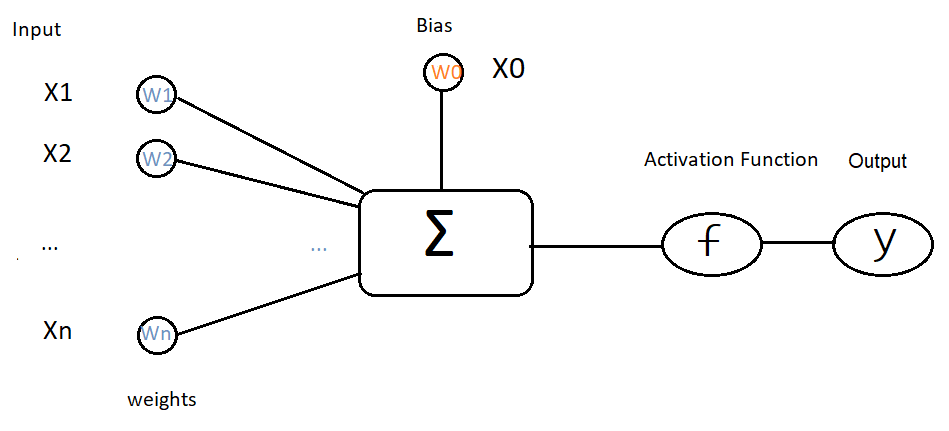
\includegraphics[height={140pt}, width={290pt}]{images/ann_mathematical_model.png}
\caption{Mathematical model for the artificial neural network's neuron}
\label{ann_mathematical_model}
\end{figure}

The purpose of the activation function is to introduce non-linearity to the architecture, which is crucial in enabling the MLP to solve most real-life problems, which are mostly non-linearly separable. For example, one of the widely used activation functions in binary problems is the sigmoid function. The sigmoid function, which is a logistic function defined for real input values, with positive derivatives everywhere and some degree of smoothness \cite{nwankpa2018activation}, has the following formula:

\begin{align*}
    \sigma(x) &= \frac{1}{(1 + \exp{-x})}
\end{align*}

Mathematically, given the outputs $x_{i}$ of the previous layer ($j$), and $n$ neurons in the current layer ($j+1$), as well as assuming a sigmoid activation function, we can define the output of the current layer as:

\begin{align*}
    y_{j+1} &= \sigma(\sum_{i=1}^{n} w_{i}*x_{i} + b_{j+1})
\end{align*}

Finally, the back-propagation algorithm used to train the MLP, updates all the weights of the neural network appropriately such that the difference between the ground truth and the network's output (the error) is as small as possible.

\begin{figure}[h]
\center
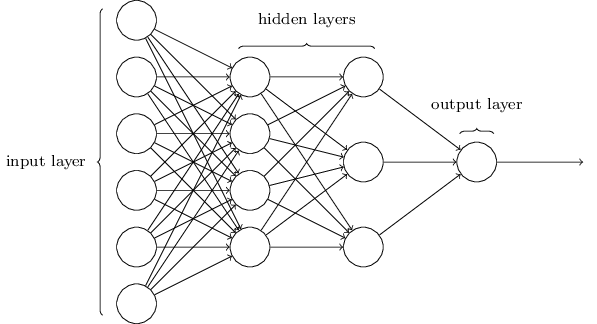
\includegraphics[height={150pt}, width={350pt}]{images/multilayer-perceptron.png}
\caption{Multi-layer perceptron neural network}
\small\textsuperscript{Image source: \href{https://computersciencewiki.org/index.php/Multi-layer_perceptron_(MLP)}{Computer Science Wiki}, (\href{https://creativecommons.org/licenses/by-nc-sa/4.0/}{CC BY-NC-SA 4.0}, unchanged)}
\label{multi_layer_perceptron}
\end{figure}

\subsection{Convolutional Neural Networks}
\label{convolutional_neural_networks_background}
A Convolutional Neural Network (CNN) is a type of deep neural network that extracts high-level hierarchical features from the raw data through convolution operations alternated with sub-sampling operations. They were first introduced by LeCun et al. \cite{lecun1998gradient} in computer vision applications.
A CNN can be considered as a special case of ANN. On principle, like the above-mentioned multi-layer perceptron (MLP), a CNN is a connected neural network with each neuron having its weight and bias where the dot product between the input and the neuron weights is feed forward. However, in difference from the typical MLP, which is a fully connected network (i.e., each neuron is connected to all the neurons of the next layer), a CNN is only locally connected to a small subset of the input data region in the grid. Some of the core concepts in a CNN architecture are the following \cite{lecun1998gradient}:

\begin{enumerate}
    \item Kernel (Filter): Typically a \textit{3x3}, \textit{5x5} or \textit{7x7} matrix with which we realize the so-called \textit{convolution operation} with the image. The convolution operation, the most important operation of CNN, consists of a matrix multiplication operation between the image and the filter. This is realized by sliding the filter in the image based on a leap number called the stride. The values of the filters are typically learned during the training process.
    \item Padding: adds additional pixels to the contours of an image, mainly in order to avoid the image drastically shrinking from the convolutional operation. The most popular choices are valid convolution where no padding is used and same convolution where the padding is chosen in such a way that the size of the output image after the convolution operation is the same as the size of the input image.
    \item Stride: The leap size when the kernel is convolved with the image. A $stride = 2$ would mean that we jump by 2 pixels whenever we apply the kernel to the image.
\end{enumerate}

The input and output dimensions of the image before and after the convolution operation are governed by the formula:

\begin{align*}
    n \times n * f \times f \rightarrow (\frac{n-f+2p}{s} + 1) \times (\frac{n-f+2p}{s} + 1)
\end{align*}

where $n \times n$ are the initial dimensions of the image, $f \times f$ the dimensions of the kernel, $p$ the padding and $s$ the stride. For example, if the input image is of shape $224 \times 224 \times 3$ and we use a $5 \times 5 \times 3$ valid convolution, with $s=1$, then the output image will be $111 \times 111 \times 1$ (after being rounded off). If we used $k$ filters, then the end result would be $111 \times 111 \times k$.

CNNs typically use multiple filters at convolutions in order to extract multiple features. The most common and successful strategy is to design a deep convolutional neural network where the height and the width of an image gradually shrink from one layer to another while the number of filters keeps increasing to pick up more complex features. This has proven successful in classical CNN studies \cite{lecun1998gradient} \cite{krizhevsky2012imagenet} \cite{simonyan2014very}. Apart from the above-described convolutional layer, a CNN consists of two additional layers: pooling layers and fully connected layers. The pooling layer typically reduces the representation size, while the fully connected layer resembles the layers of a multi-layer perceptron network. One layer of a CNN typically consists of one or more convolutional layers followed by a pooling layer. Figure \ref{cnn_block} represents such a layer.

\begin{figure}[h]
\center
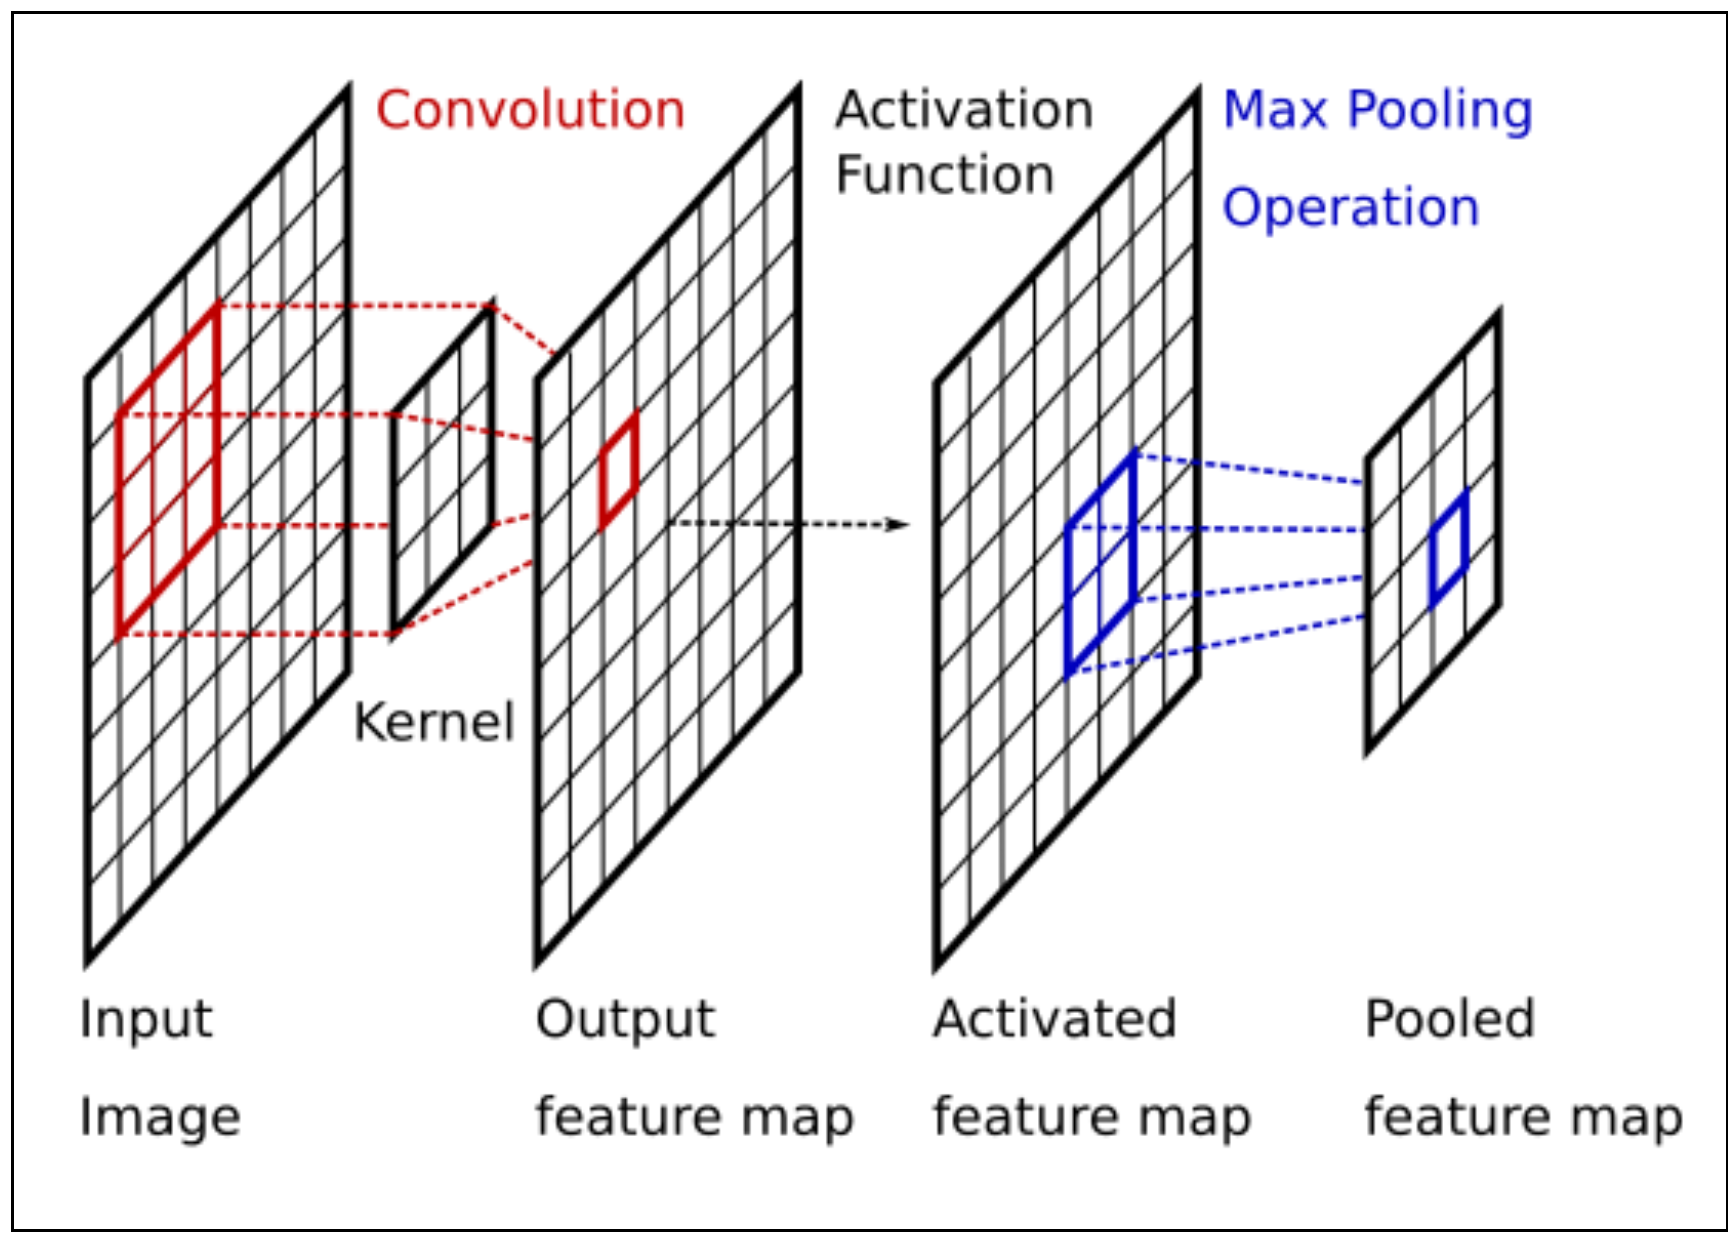
\includegraphics[height={150pt}, width={300pt}]{images/cnn_block.png}
\caption{Basic CNN block consisting of a single convolutional operation, followed by an activation function and max pooling operation \cite{georgiou2020survey}}
\label{cnn_block}
\end{figure}

Similar to the architecture of the MLP, CNN is comprised of an input layer, multiple hidden layers in the form of convolutional or pooling layers, and an output layer in the form of a fully connected layer. The three main advantages of CNN over ANN are:
\begin{enumerate}
    \item Structure: inspired by the human visual processing system and is highly optimized for processing images.
    \item Parameter sharing: the sharing of weights by all neurons in a particular feature map.
    \item Sparsity of connections: CNN typically uses much fewer parameters than an equivalent Deep Neural Network. This is computationally more feasible but also avoids overfitting.
\end{enumerate}

However, CNN typically require powerful computing capabilities, which is nowadays facilitated by the use of GPU, might overfit the data if the dataset is not big enough, i.e. they usually require big datasets \cite{krizhevsky2012imagenet}, and occasionally suffer from disappearing or crashing gradients. The three main layers of a typical CNN are illustrated below:

\bigskip
\noindent\textbf{Convolution Layer}: Applies several kernels to the input image in order to extract features. Stacking more than one convolutional layer with each other allows the extraction of higher-level features. For example, the first convolutional layer might extract low-level features such as edges, while the second might extract shapes like circles or squares with yet a deeper one extracting shapes of eyebrows or noses. The output of the convolution is then passed to a non-linear activation function such as sigmoid, softmax or relu \cite{nwankpa2018activation}, which is crucial for learning.

\bigskip
\noindent\textbf{Pooling Layer}: The purpose of the pooling layer is to reduce the dimensions of the image as it is feed through the network and make the computations lighter. However, the most important function of the pooling layer is to make some of the detected features more robust, that is to say to further highlight them. The most widely used types of pooling are max-pooling and average-pooling. The idea is that after a feature is detected during the convolution operation, the pooling operation preserves and highlights it. Figure \ref{max_pooling} shows a max-pooling operation that preserves the maximum activations of a $4 \times 4$ matrix. These activations would correspond to a detected feature.

\begin{figure}[h]
\center
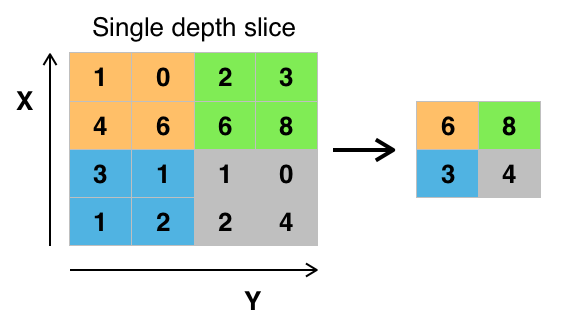
\includegraphics[height={150pt}, width={220pt}]{images/max_pooling.png}
\caption{Max Pooling with a kernel size $2 \times 2$ \cite{georgiou2020survey}}
\label{max_pooling}
\end{figure}

\bigskip
\noindent\textbf{Fully Connected Layers}: After features have been extracted in a series of convolutions and pooling layers, we flatten the output and feed it to one or more fully connected (FC) layers. The final FC layer would be the layer that performs the prediction. For example, for a digit recognition problem, the output layer would consist of 10 neurons representing the numbers $0-9$, and we would apply a soft-max activation function \cite{nwankpa2018activation} for the ten possible outputs.

\bigskip
\noindent Convolutional neural networks have proved themselves state-of-the-art algorithms in many Machine Learning problems. Their applications include, but are not limited to, image classification \cite{he2016deep}, object detection \cite{redmon2018yolov3}, pose estimation \cite{toshev2014deeppose}, segmentation \cite{cao2019gcnet} as well as other areas outside computer vision such as robotics or natural language processing.

\subsubsection{2D Convolutional Neural Networks}
\label{2d_convolutional_neural_networks_background}

2D Convolutional Neural Networks (2D CNN) are CNNs that consist of convolutions with 2D kernels. The most prominent example would be spatial convolutions over images. The convolution is done by computing the sum of the dot product between input data and the kernel. We stride the kernel over the input data, as explained in the previous section. After the bias is added, the convolutional features are passed through an activation function of choice. One or more convolutional layers are then followed by a pooling layer, which reduces the resolution of the feature maps. Figure \ref{alexnet} illustrates AlexNet, a seminal work in image recognition, which popularized the use of Deep Learning in computer vision \cite{krizhevsky2012imagenet}. It applies five convolutional layers followed by max-pools at different points. The first layer, for example, applies 96 $11 \times 11 \times 3$ filters with a stride of 4 on the rgb input image, giving as output a $55 \times 55 \times 96$ volume. This volume is then passed through a max-pooling layer with a $3 \times 3$ filter that further reduces the dimensions to $27 \times 27 \times 96$. More convolution and pooling layers are applied until the volume is flattened, and two FC layers are applied before it uses a Soft-Max function of 1000 nodes that correspond to each of the 1000 classes in the Image-Net dataset. The network has 60M parameters, which would normally make it very computationally intensive; however, the efficient use of GPU makes the training process feasible. It further uses a Re-Lu activation function \cite{glorot2011deep} and dropout regularisation \cite{hinton2012improving}, which made it a very efficient network for its time.

\begin{figure}[h]
\center
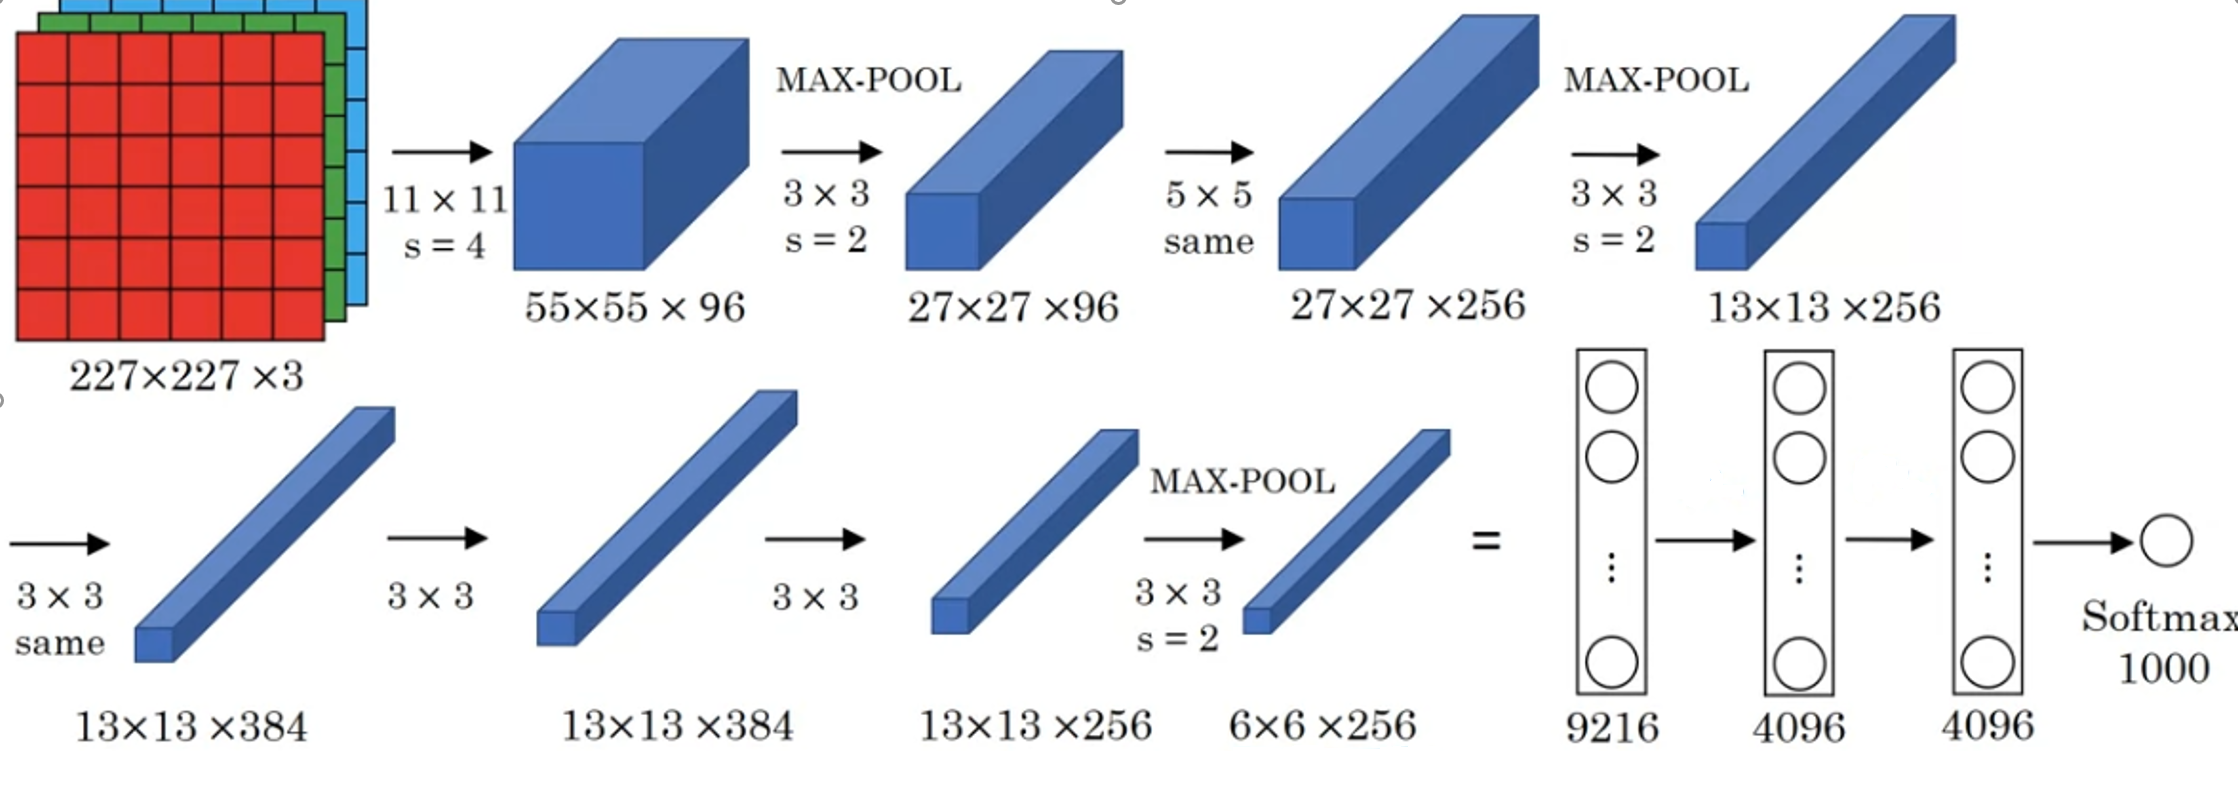
\includegraphics[height={160pt}, width={440pt}]{images/alexnet.png}
\caption{AlexNet}
\small\textsuperscript{Image source: \href{https://www.coursera.org/learn/convolutional-neural-networks}{CNN at Coursera by Andrew Ng}}
\label{alexnet}
\end{figure}

\subsubsection{3D Convolutional Neural Networks}
\label{3d_convolutional_neural_networks_background}

Using 2D-CNN has a pronounced disadvantage in videos: they ignore the temporal dimension of a video and hence cannot fully capture the developing motion. Especially when it comes to human action recognition and its nuances, if we only look at an image's spatial dimensions, we will be missing the richness of information that videos usually contain. For instance, 2D ConvNets cannot tell the difference between opening or closing a door, given that all they work with is static frames. 3D ConvNets use 3D kernels and can extract Spatio-temporal features from continuous frames, which makes them a natural choice for video activity recognition \cite{ji20123d}. This model convolves 3D kernels to the cube formed by stacking multiple continuous frames together. Since this cube contains multiple frames, the convolutional operation can extract motion information as well. Like 2D ConvNets, where one kernel only picks up a particular feature, we need to stack 3D kernels to extract more features. However, this also means that a 3D ConvNet has many more parameters than a 2D ConvNet and is more computationally intensive. The implementation of 3D max-pooling preserves the spatio-temporal information at subsequent layers.

Figure \ref{3d_feature_extraction} shows the feature extraction from contiguous frames by using multiple 3D kernels to extract multiple features. The set of connections are color coded to show shared weights in the same color. Because the six sets of connections do not share weights, we get two different feature maps on the right.

\begin{figure}[h]
\center
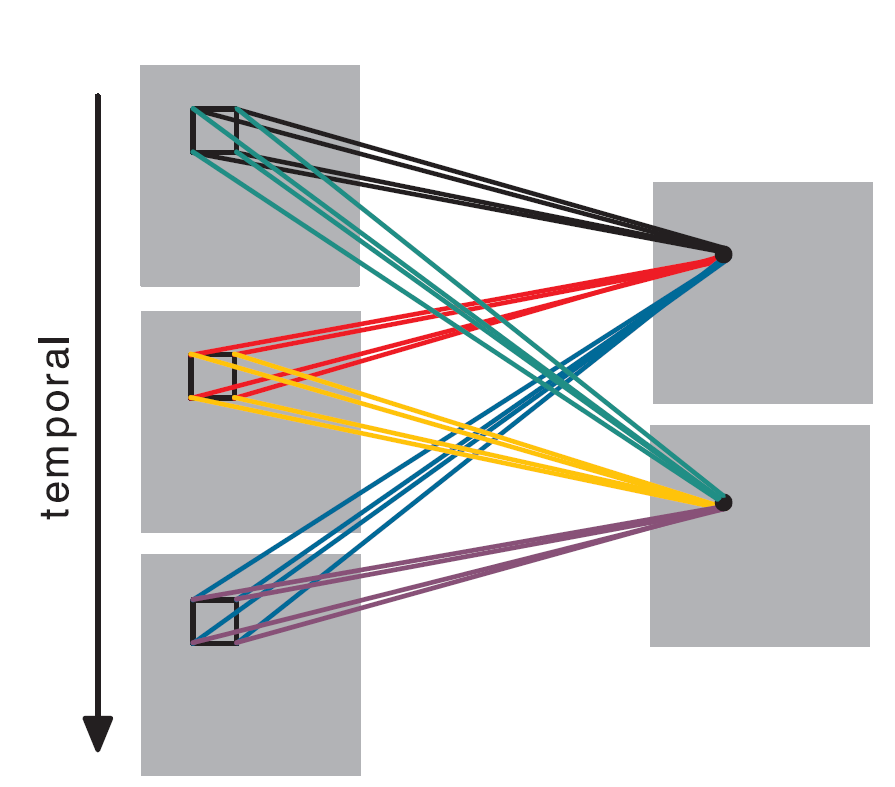
\includegraphics[height={160pt}, width={240pt}]{images/3d_feature_extraction.png}
\caption{Feature extraction by 3D kernels \cite{ji20123d}}
\label{3d_feature_extraction}
\end{figure}

The general construct remains the same as with 2D ConvNets: we increase the number of feature maps in late layers by creating multiple types of features from the same set of lower-level maps, whilst at the same time decreasing the overall shape of the volume until we flatten the result and connect it to the final head classifier with an activation function of choice. \cite{tran2015learning} produced the first 3D ConvNet architecture with clearly superior performance over previous 2D ConvNet architectures. They found that a homogenous architecture with $3 \times 3 \times 3$ convolutional kernels in all layers was among the best performing architectures for 3D ConvNets. Figure \ref{2d_3d_convs} illustrates the difference between the 2D and 3D convolutional operation. Applying 2D convolutions on images results in another image in $(a)$. It remains the same with applying 2D convolution to a video volume with multiple frames in $(b)$. However, applying a 3D convolution on a video volume will only in another video volume as shown in $(c)$. This makes sure that the temporal information is preserved.

\begin{figure}[h]
\center
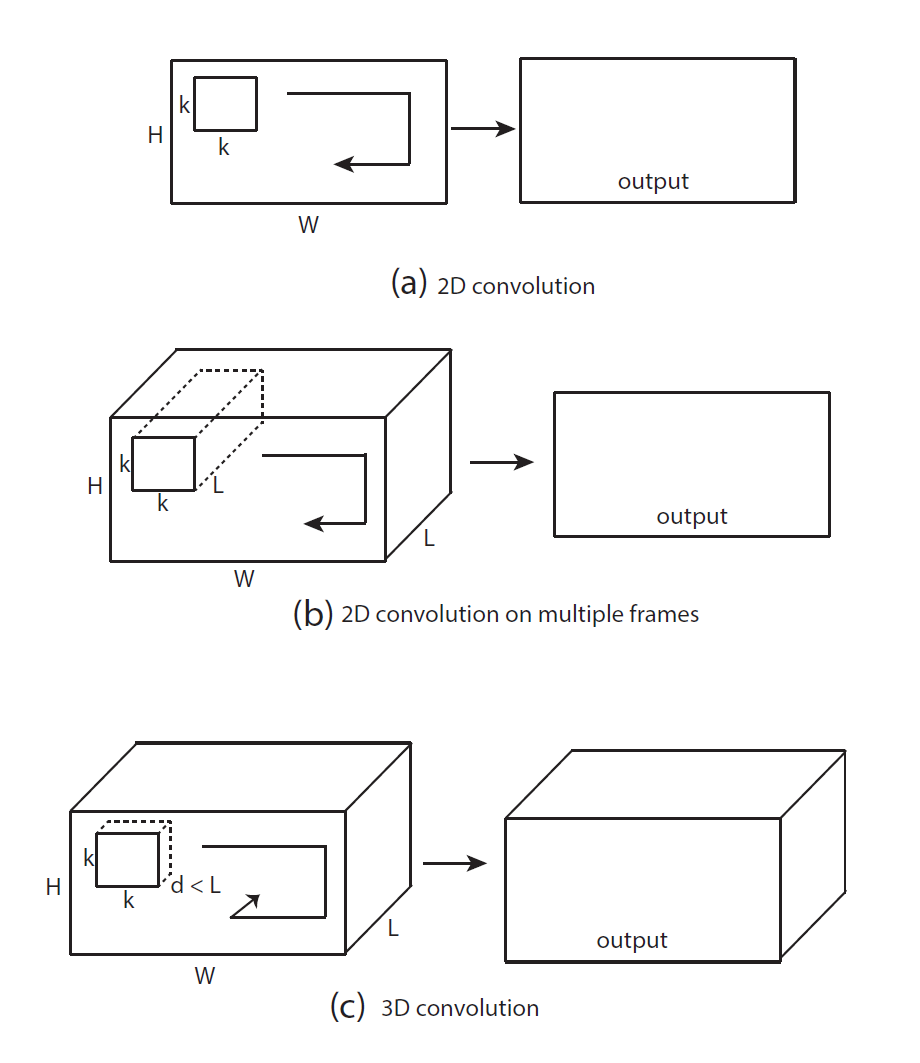
\includegraphics[height={300pt}, width={260pt}]{images/2d_3d_convs.png}
\caption{2D vs 3D convolution operation \cite{tran2015learning}}
\label{2d_3d_convs}
\end{figure}

As with the MLP and 2D ConvNets, training a 3D ConvNet involves two phases: Feed-forward and updating. The feed-forward consist of feeding a sample thorough the network, through the various convolutional, pooling, activation or fully-connected layers in order to receive the final result. The update phase then refers to the fiddling of the weights through a back-propagation algorithm in order to reduce the error in the output of the network. The loss error in the output layer is calculated by using a loss function of choice. In this thesis, a softmax classifier with a cross-entropy loss function was used for the heads of the networks.  The cross-entropy loss has the form\footnote{Softmax classifier --- \url{https://cs231n.github.io/linear-classify/#softmax-classifier}}:

\begin{align*}
    L_{i} &= -\log \left(\frac{\exp{f_{y_{i}}} }{\sum_{j} \exp{f_{j}}} \right)
\end{align*}

where $f_{j}$ is the \textit{j-th} element of the vector of class scores $f$ and the mean of $L_{i}$ over all training samples is the full loss of the dataset. The output of of the softmax is a normalized class probability for each of the final neurons corresponding to each label in the classification problem. The target class has the highest probability. It has the form:

\begin{align*}
    f(x_{i}) &= \frac{\exp{x_{i}}}{\sum_{j} \exp{x_{j}}}
\end{align*}

The softmax function takes a vector of real value scores ($x$) and squashes it to a vector of values between zero and one that sum to one.

\subsection{Skeleton Based Action Recognition}
\label{background_skeleton_based_ar}

This thesis uses three modalities for feature representation, namely RGB frames, and optical flows, which are exploited by the above-discussed neural networks, and finally pose data to form human skeletons. Due to the fact that skeleton-based action recognition entirely focuses on human action, it has achieved increasing attention in the computer vision community in recent years. Indeed common problems with video understanding such as background variation and lightning changes do not exist when using human poses. These skeletons are commonly represented as a sequence of human joint coordinate list, where the coordinates are extracted by pose-estimation methods \cite{duan2021revisiting}. Various methods have been employed for skeleton-based action recognition \cite{du2015hierarchical},\cite{vemulapalli2014human}. 

\cite{du2015hierarchical} for example, constructed an end-to-end hierarchical RNN that separated the human body into five parts and took them as input to the model. However, the most popular approaches have been graph convolutional networks (GCN) that extract features on top of human skeletons \cite{yan2018spatial}. GCN regards every human joint at every timestamp as a node. Neighboring nodes are then connected with edges along the spatial dimension and along the temporal one. This forms the input fed to the GCN, thus utilizing information across space and time. Such models have been shown to yield a good performance on common benchmark datasets.

Recently a work by \cite{duan2021revisiting} suprassed the GCN-based methods both in terms of performance but also robustness, interoperability and scalability. This was the chosen skeleton-based HAR model in the context of this work, and is examined in details in Section \ref{skeleton_models}.


\newpage
\section{Literature Review}
\label{literature_review}

Over the past few decades, there have been two major avenues for research in video understanding. Before deep learning became ubiquitous, the first one concerns the use of hand-crafted features in conventional machine learning methods. In this respect, various methods have been employed with various rates of success. The most successful of these methods have been random forests (RF) \cite{breiman2001random}, support vector machines (SVM) \cite{cortes1995support} and optical flow (described in Section \ref{background_optical_flow}). For example, \cite{gan2013human} employed random forests with a binary tree architecture on 3D skeleton joints extracted from depth image, while support vector machine multi-class classifiers were utilized by \cite{qian2010recognition} achieving good results when the number of samples was small. 

The second branch of research concerns the use of deep learning architectures, which have proven state-of-the-art in many domains and are the focus of this work. More specifically, one can reap from deep learning techniques the following benefits when compared to conventional ML methods:

\begin{enumerate}
    \item Conventional ML methods rely heavily on feature extraction via heuristics and other hand-crafted techniques. This means that domain expertise is needed for such methods to work, and success is not guaranteed. On the other hand, DL methods can automatically learn features, provided that there is enough data, as explained in detail in Section \ref{artificial_neural_networks_background}. Moreover, the likelihood of success with these methods is much higher, especially given the tremendous amount of energy put into this branch of research in the last decade, which has improved many aspects of the deep learning methods.
    \item The features learned by DL techniques are usually more superior to any hand-crafted features.
    \item Conventional ML methods might perform good for basic activities such as \textit{walking} or \textit{running}. However, their performance seriously degrades for more complex activities such as \textit{drinking coffee} or \textit{baking cookies}. DL techniques, on the other hand, have solved these harder activities.
    \item ML methods are prone to learning from static data, while DL methods can learn from streaming data and incrementally improve. This could be useful in the context of the \textit{Vortanz} project as well.
    \item A dataset can be labeled by unsupervised DL methods, thus increasing the amount of data that the models can utilize.
    \item Finally, transfer learning \cite{shaha2018transfer}, makes DL techniques incredibly robust when working in various domains.
\end{enumerate}

\noindent For these reasons, this work focuses on DL techniques and disregards the more conventional algorithms. This chapter presents an overview of the deep learning architectures that were used in this thesis. Deep learning, perhaps the most important subfield of machine learning, aims to learn multiple representations and abstraction levels in order to make sense of data like images, text or speech. As explained in Section \ref{convolutional_neural_networks_background},  deep convolutional neural networks treat images in their raw form and automatically extract, represent and classify features from them without the need for expert domain knowledge to manually construct such features as is the case with more conventional machine learning methods for example. Deep learning architectures utilize trainable feature extractors and computational models with multiple processing layers to represent and recognize labels. With the rise of deep learning in computer vision in the previous decade, it has also been successfully used for human activity recognition. Current state-of-the-art models are such deep learning models and are able to learn complex human actions, which were not possible with other methods before. Deep learning approaches incorporate both the feature extraction (also known as the \textit{backbone}) as well as the classification (also known as the \textit{head}) phase into a single architecture. Two main instances of deep learning techniques in HAR, which are also the focus of this thesis, are convolutional and recurrent neural networks (RNN). 

\bigskip
\noindent This thesis does not aim to develop new deep learning architectures but rather to try existing and state-of-the-art architectures in the given domain. Three families of models have been utilized with great success so far in HAR, namely two-stream, 3D ConvNets, and skeleton-based models. This thesis tries different architectures from all of these. Following, an overview of utilized 2D- and 3D-ConvNets is given in Sections \ref{2d_convolutional_models} and \ref{3d_convolutional_models} respectively as well as a brief overview of the used skeleton model at Section \ref{skeleton_models}. The networks are discussed according to the timeline of their appearance in the literature.

\subsection{2D Convolutional Models}
\label{2d_convolutional_models}

\noindent\textbf{Temporal Segment Network (TSN)}: composed of spatial stream ConvNets operating on single RGB images that extract spatial imformation from frames and temporal stream ConvNets operating on a stack of consecutive optical flows, that extract information from the temporal dimension \cite{wang2016temporal}. Figure \ref{tsn_structure} illustrates the architecture of TSN that combines these two streams. They employed for the first time a uniform sampling technique of frames that splits the input video into $k$ segments and then samples one frame from each of these segments. This drastically improved the computational performance of TSN when compared to previous work such as \cite{tran2015learning} and later became a common practice in 2D models.

\begin{figure}[h]
\center
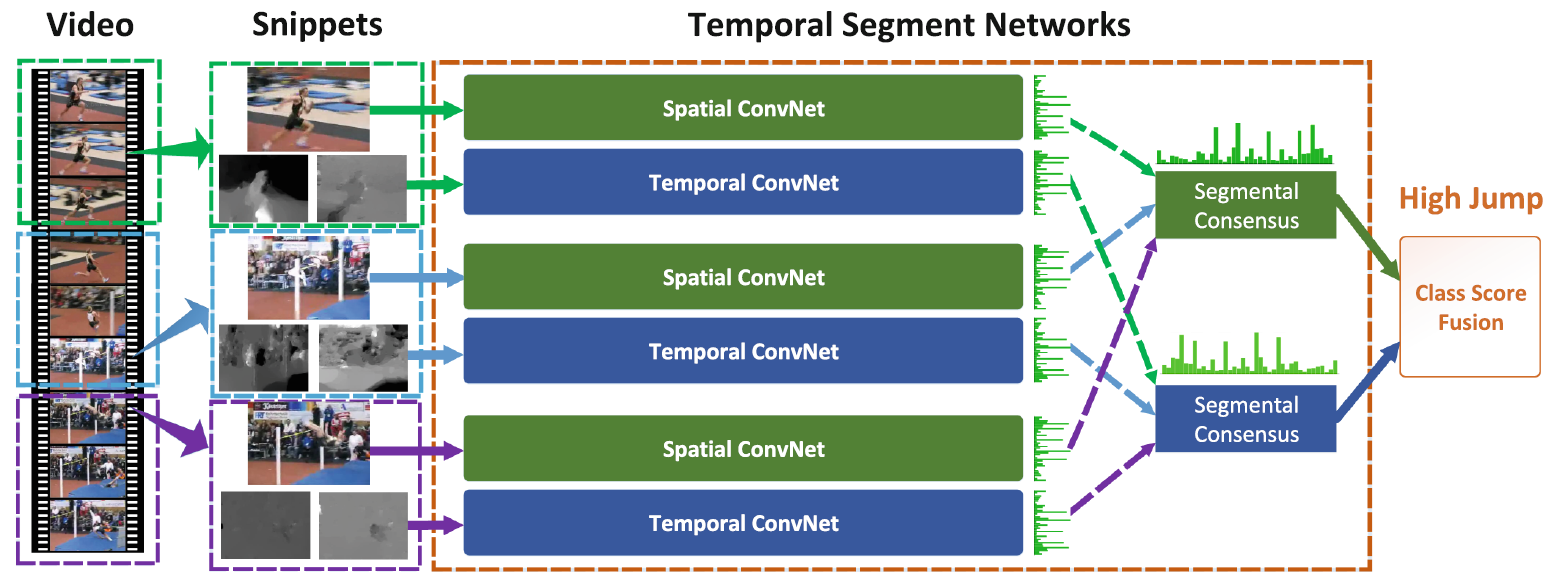
\includegraphics[height={190pt}, width={430pt}]{images/tsn_structure.png}
\caption{TSN structure \cite{wang2016temporal}}
\label{tsn_structure}
\end{figure}

\bigskip
\noindent\textbf{Temporal Relational Reasoning (TRN)}: developed by \cite{zhou2018temporal} learns and reasons about the temporal dependencies between video frames at multiple time scales. For example, \textit{sprinting} consists of long-term relations such as \textit{crouching}, \textit{running} or \textit{finishing} and of short-term relations such as periodic hand and feet movement. This type of module becomes very useful for temporal related actions such as \textit{dropping something into something} or \textit{pushing something with something} \cite{goyal2017something}.

\bigskip
\noindent\textbf{Temporal Shift Module (TSM)}: proposed by \cite{lin2019tsm} in order to find the best of both worlds between low computation cost but insufficient 2D ConvNet modeling of videos and more accurate but the higher computational cost of 3D ConvNet modeling. TSM realizes this by shifting part of the channels along the temporal dimension to facilitate the information exchanged between neighboring frames. Thus, it can use 2D convolutions for better computational performance while exploiting information from the temporal dimension since it has shifted some of the channels to emulate 3D convolutions. Figure \ref{tsm_block} illustrates this. It shows the original tensor with its channels intact and then after fiddling with the temporal dimension. The shift can be forwards and backward for offline inference or only forwards for online inference.

\begin{figure}[h]
\center
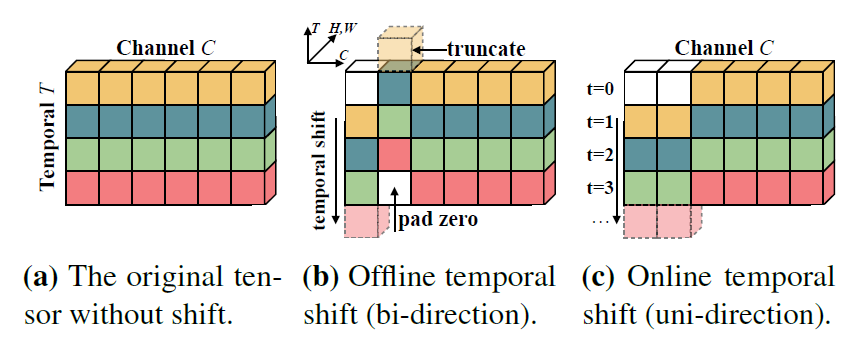
\includegraphics[height={110pt}, width={265pt}]{images/tsm_block.png}
\caption{TSM block \cite{lin2019tsm}}
\label{tsm_block}
\end{figure}

\bigskip
\noindent\textbf{Temporal Adaptive Module (TAM/TANet)}: An architecture that focuses on devising a temporal module that is both efficient but also flexible \cite{liu2020tam}. Its main critique against 3D convolutions is that a fixed number of video invariant kernels might not be enough to capture the temporal diversity of videos and that subtler tricks should be employed instead. Hence in order to address this problem, a new temporal adaptive module (TAM) is presented. TAM poses a two-level adaptive modeling capability: An importance map, which is learned in the local temporal window to capture short-term information and an aggregation weight generated from a global view and focuses on the long-term structures.

\bigskip
\noindent\textbf{Temporal Interlacing Network (TIN)}: Similar to TSM, a method was developed to combine the spatial and temporal information into a single one only to learn it once \cite{shao2020temporal}. This was achieved by interlacing spatial information from the past to the future and vice-versa. Figure \ref{tin_block} illustrates how the temporal information is utilized by interlacing spatial representations in the temporal dimension. This fused representation is then processed in later network layers. In this way, TIN does not have to perform expensive 3D convolutions to extract features from the temporal dimension.

\begin{figure}[h]
\center
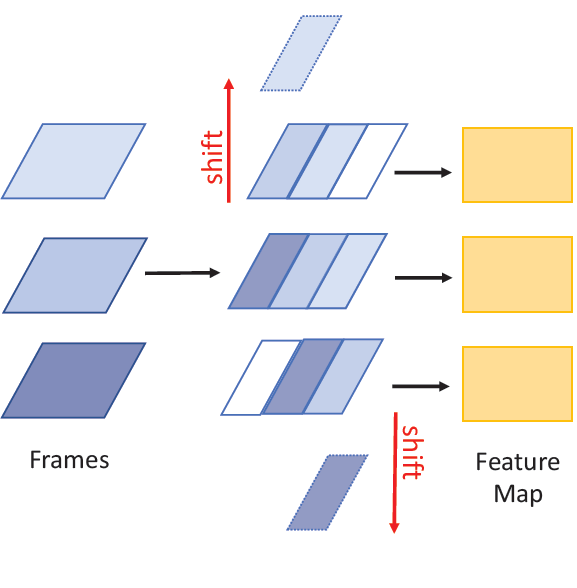
\includegraphics[height={180pt}, width={145pt}]{images/tin_block.png}
\caption{Interlacing of spacial representations \cite{shao2020temporal}}
\label{tin_block}
\end{figure}

\subsection{3D Convolutional Models}
\label{3d_convolutional_models}

\noindent\textbf{Two-Stream Inflated 3D ConvNets (I3D)}: A classical work in HAR that shows the potency of 3D convolutions \cite{carreira2017quo}. It uses two streams. The first stream takes RGB frames as an input modality and passes them through a 3D ConvNet. This 3D ConvNet consists of inflated 2D kernels and pooling layers of very deep image classification networks into 3D in order to be able to exploit the temporal dimension. The second stream is an optical flow stream, which further improves the network's ability to detect actions. Figure \ref{i3d_architecture} illustrates this architecture. Thus this model leverages, first of all, the state-of-the-art ConvNet architectures from the image recognition domain (by converting them to 3D models), and second their pre-trained weights on the ImageNet dataset. It achieved the best results in the Kinetics dataset at the time that it came out.

\begin{figure}[h]
\center
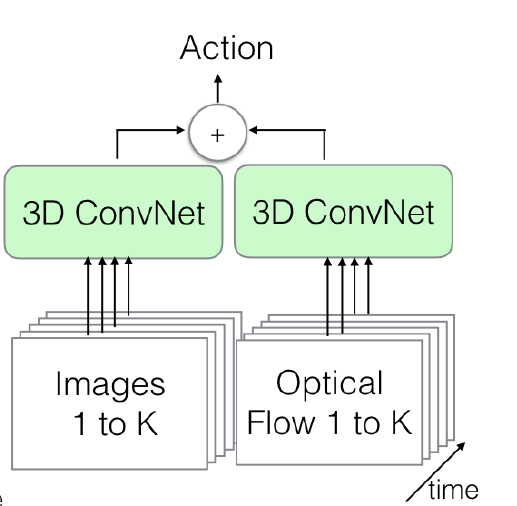
\includegraphics[height={150pt}, width={145pt}]{images/i3d_architecture.png}
\caption{Two-Stream 3D-ConvNet \cite{carreira2017quo}}
\label{i3d_architecture}
\end{figure}

\bigskip
\noindent\textbf{Channel-Separated Convolutional Networks (CSN)}: In order to reduce the computational intensity of 3D ConvNets, different ways of factorizing 3D convolutions into group convolutions are studied \cite{tran2019video}. This is achieved by decomposing 3D convolutions into either pointwise $1 \times 1 \times 1$ for channel interaction or depthwise $k \times k \times k$ for local spatiotemporal interaction convolutions. The paper introduces two kinds of factorizations: \textit{interaction-reduced} and \textit{interaction-preserved}. Incidentally, such factorizations also act as regularizers, that is these models have a higher training error but better generalization capabilities, which is what we typically want when solving an ML problem. Figure \ref{csn_architecture} illustrates the new factorizations. In $(a)$ we see the conventional convolutional block, which is transformed in $(b)$ and $(c)$. $(b)$ shows an \textit{interaction-preserved} block where the original $3 \times 3 \times 3$ block has been decomposed into a block consisting of a $1 \times 1 \times 1$ traditional convolution and a $3 \times 3 \times 3$ depthwise convolution. The block improves the computational performance when compared to $(a)$ but also preserves most channels interactions via the newly added channel interaction $1 \times 1 \times 1$ convolution. Similarly we have in $(c)$ an \textit{interaction-reduced} blocked where we remove the $1 \times 1 \times 1$ convolution and are only left with the local spatiotemporal $3 \times 3 \times 3$ depthwise convolution. This block has a reduced number of channel interactions when compared with $(a)$ or $(b)$ and is therefore more computationally light than them, which comes at a slight trade-off of performance.

\begin{figure}[h]
\center
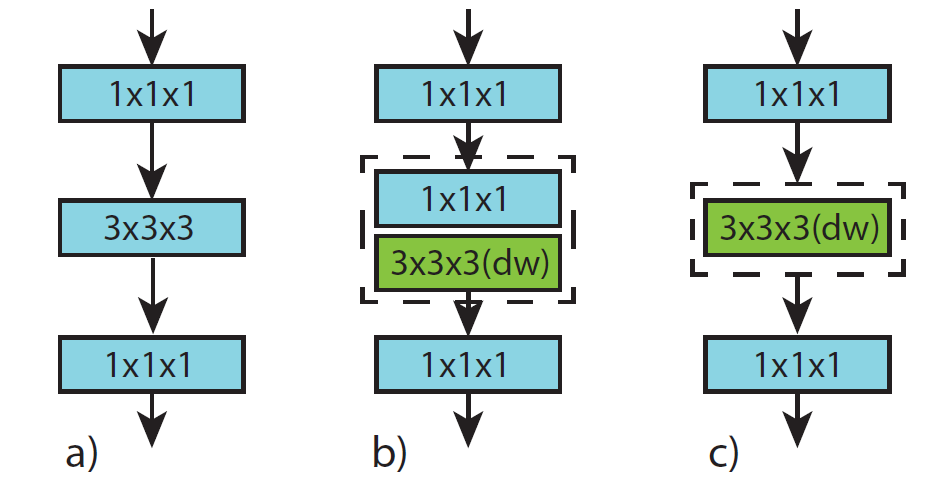
\includegraphics[height={110pt}, width={180pt}]{images/csn_architecture.png}
\caption{Standard vs. channel-separated convolutional blocks \cite{tran2019video}}
\label{csn_architecture}
\end{figure}

\bigskip
\noindent\textbf{SlowFast}: A model that has two pathways, a Slow pathway that operates at object level, that is captures spatial semantics, and a Fast pathway that operates at action level, that is, captures temporal semantics \cite{feichtenhofer2019slowfast}. The motivation behind this architecture is the observation that the world is mostly at rest, which makes slow motions much more prevalent than faster motions. Hence, SlowFast treats space-time asymmetrically, unlike I3D. As shown in Figure \ref{slowfast_architecture}, the Slow path operates at a low frame rate but a high channel rate, enabling it to capture spatial semantics. The Fast pathway then operates on a high frame rate but low channel rate (which makes it very lightweight), and this enables it to capture motion at the temporal dimension. The two paths are finally merged through late fusion to procure the final prediction.

\begin{figure}[h]
\center
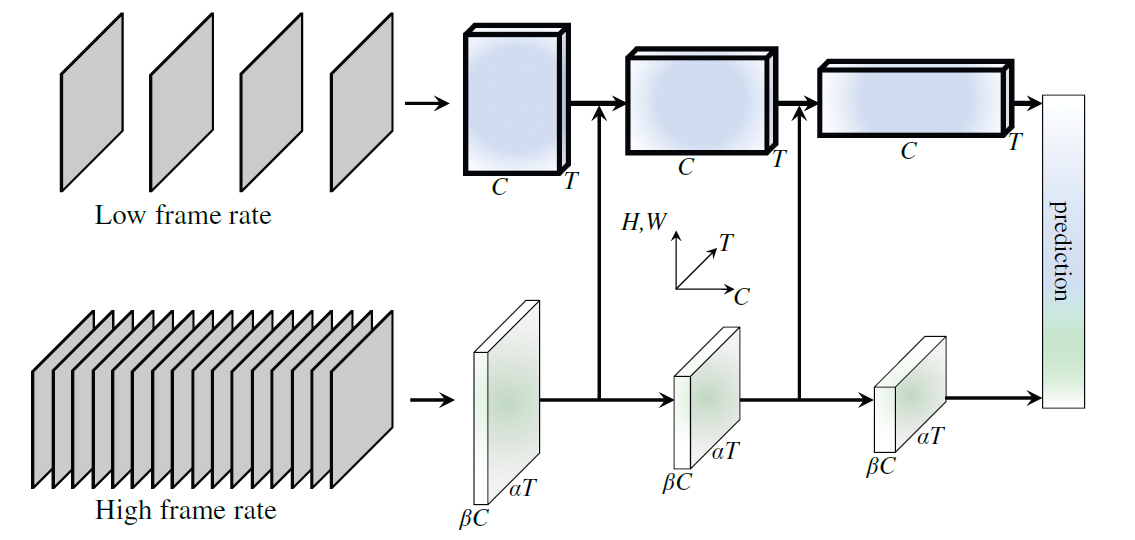
\includegraphics[height={150pt}, width={270pt}]{images/slowfast_architecture.png}
\caption{The architecture of SlowFast. Slow pathway on top and fast below. \cite{feichtenhofer2019slowfast}}
\label{slowfast_architecture}
\end{figure}

\subsection{Skeleton Models}
\label{skeleton_models}
\noindent\textbf{PoseC3D}: sets the new state-of-the-art HAR model that utilizes skeleton data as of 2021 \cite{duan2021revisiting}. Figure \ref{posec3d_architecture} illustrates the architecture of PoseC3D. After the person or people in the frame are detected, a 2D pose extraction model extracts 17 keypoints, which are then reformulated as 2D heatmaps of skeleton joints. These 2D heatmaps are then stacked sequentially to form 3D heatmap volumes, then fed to a deep 3D ConvNet. The paper shows that PoceC3D outperforms GCN-based approaches while alleviating their robustness, interoperability, and scalability limitations. Hence, GCN-based approaches were not utilized in the context of this thesis.

\bigskip
\noindent Two different networks are designed: \textit{Pose-Slow-Only} and \textit{RGB-Pose-SlowFast}. The former is inspired by the Slow pathway of SlowFast and uses only pose data. The latter contains both the Slow and Fast pathway, which process the RGB and Pose modalities. After that, the predictions of the two pathways are combined in a late-fusion manner. This thesis only used the former model that only utilizes pose data.

\begin{figure}[h]
\center
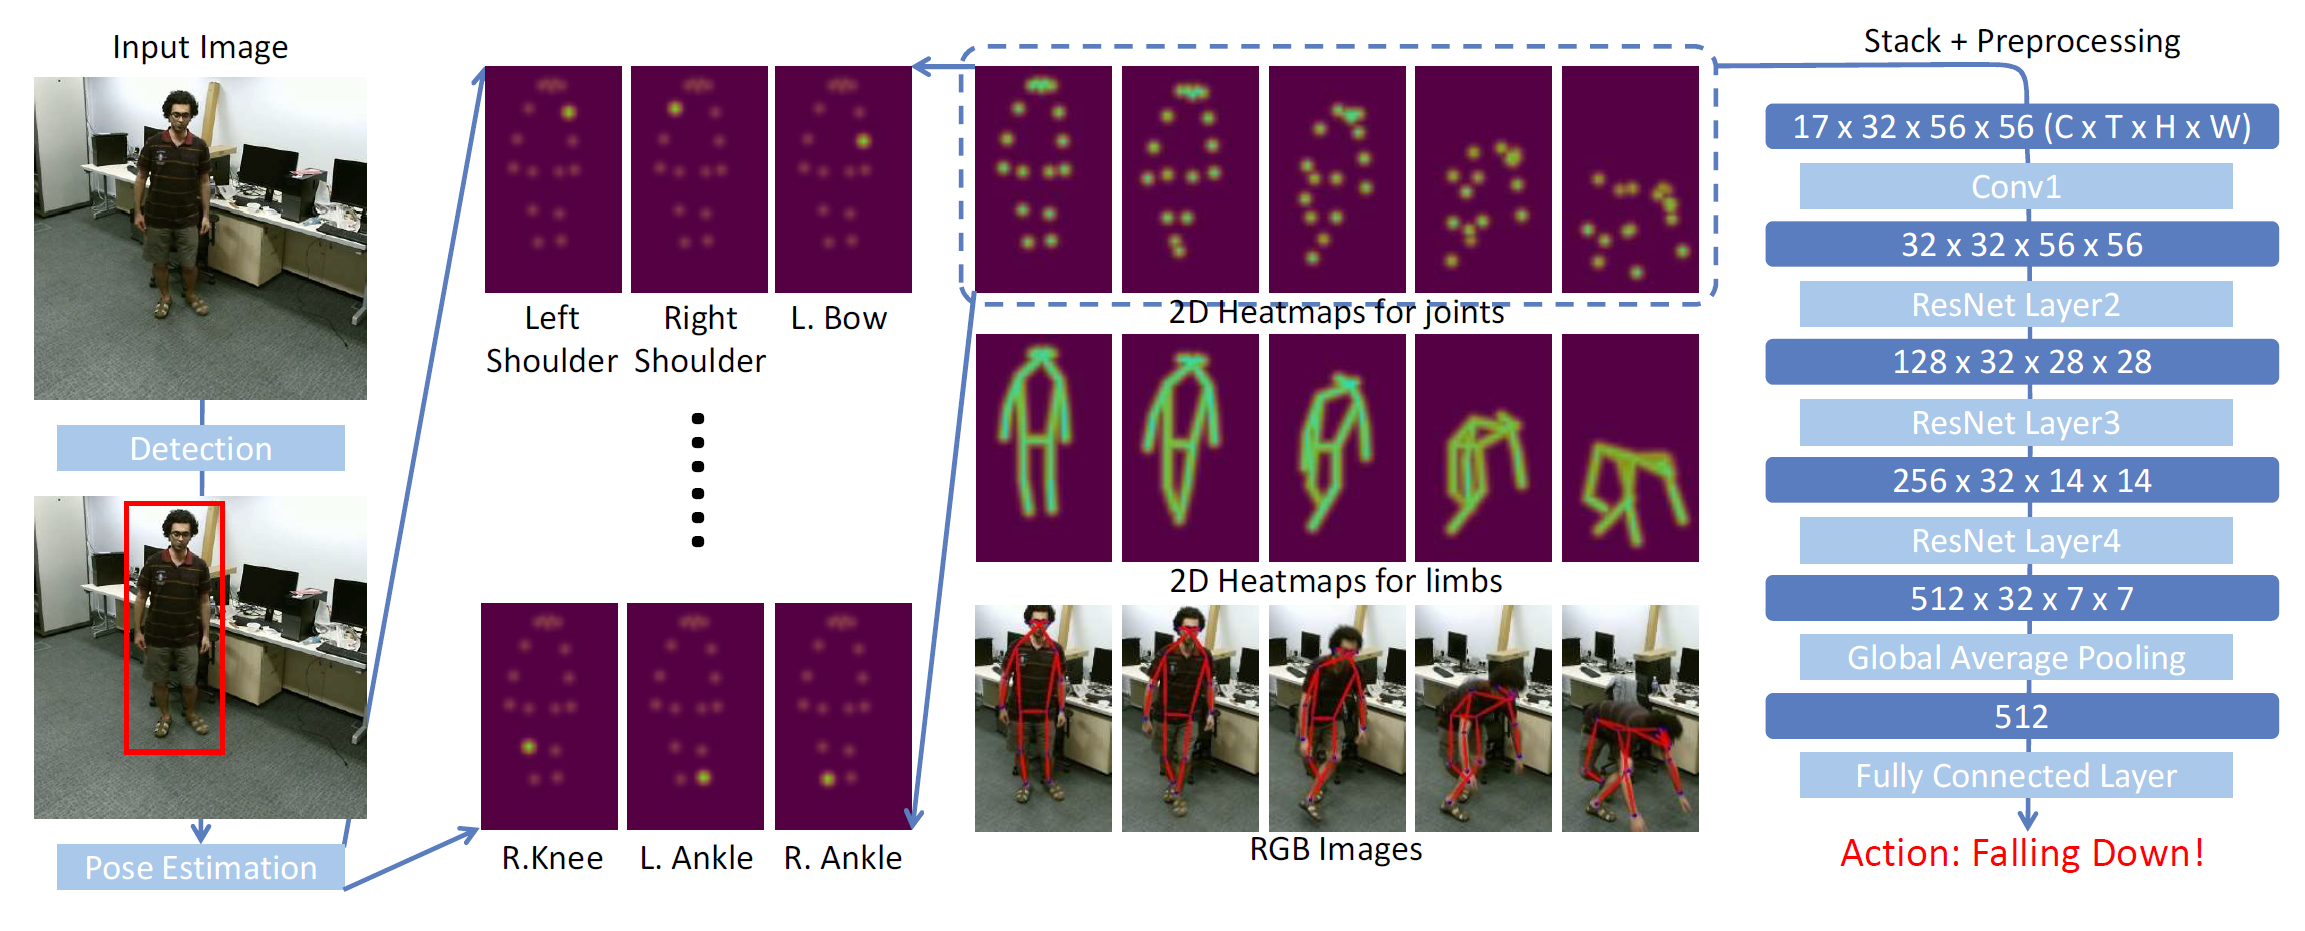
\includegraphics[height={190pt}, width={440pt}]{images/posec3d_architecture.png}
\caption{Architecture of PoseC3D \cite{duan2021revisiting}}
\label{posec3d_architecture}
\end{figure}

\newpage
\section{Experimental Setup}
\label{experimental_setup}

Most of the experiments concerned with the model architecture, training, validation, testing, and related plots were performed using four OpenMMLab\footnote{OpenMMLab Website --- \url{https://openmmlab.com/home}} codebases. OpenMMLab is a family of open-source projects for academic research and industrial applications covering a wide range of computer vision research topics. The main code base that was used for human action recognition is MMAction2 \cite{2020mmaction2}, while MMPose \cite{mmpose2020} was used for pose estimation and MMDetection for human detection \cite{mmdetection}. Denseflow \cite{denseflow} was used for optical flow extraction. The underlying deep learning framework on which OpenMMLab operates is PyTorch \cite{NEURIPS2019_9015}, and other related experiments, like for instance the background replacement, were written mostly based on PyTorch.

Finally, all experiments, model parameters, and metrics were tracked using MLflow \cite{zaharia2018accelerating}, which is a platform that manages the complete life-cycle of machine learning applications.

The source code is available on github\footnote{Thesis Code --- \url{https://github.com/rlleshi/thesis-har}}. However, the dataset is not publicly available due to privacy concerns.

\bigskip
\noindent This section describes the necessary experimental setup that oversees the execution of all the experiments in Section \ref{experiments}. Section \ref{bast_data} discusses the two main datasets used for model training in this thesis. Initial pre-processing, dataset split, and finally, the various input modalities, particularly the pose data, are examined in detail. Next, Section \ref{domain_testing_dataset} introduces the two datasets that were used as domain testing datasets for the experiment in Section \ref{research_question_3}. Section \ref{benchmark_datasets} briefly discusses the benchmark datasets that were examined in the research question dealing with transfer learning at Section \ref{research_question_4}. Section \ref{dl_pipeline} discusses the deep learning pipeline and model architecture setup. Finally, Sections \ref{interpretability} and \ref{model_evaluation} discuss the interpretability and evaluation criteria of the trained models respectively.

\subsection{Datasets}
\label{bast_data}
With the BAST analysis discussed in details at Section \ref{intro_bast_laban} we now turn our attention to the dataset at the disposal of this study. The dataset consists of 98 student-athletes (German and Japanese), who were recorded while performing a 10-minute two part movement test from the BAST analysis. 

The first part consists of nine basic standardized tasks: \textit{walk} (Figure \ref{walk_heatmap}), \textit{run}, \textit{jump} (Figure \ref{jump_time_long}), \textit{stamp}, \textit{contract-expand} (Figure \ref{bast_contract_expand}), \textit{tiptoe}, \textit{swing-upper-body} (Figure \ref{flow_swing_figure}), \textit{rotate} (Figure \ref{rotate_pose}) and \textit{fall} (Figure \ref{fig:fall_no_background}). These tasks were then evaluated by certified professionals based on criteria such as \textit{floor pattern}, \textit{time in air}, \textit{emphasis}, \textit{body involvement} etc. as enumerated and explained in great lengths at Section \ref{background_bast}. Figure \ref{jump_time_long} shows an example of the \textit{jump} task which was evaluated as \textit{long in time} given that the subject was performing high jumps. In total 42 out of a total of 63 annotations (for an explanation refer to Section \ref{insufficient_data}) were taken into account from the evaluation of the nine basic standardized tasks. Each video from this task is accompanied by annotations in XML format, which indicate the performed actions with their corresponding timestamps.

\bigskip
\noindent The second part of the BAST analysis consists of four one-minute improvisation tasks, where the students were asked to emulate \textit{water}, \textit{fire}, \textit{air} and \textit{earth}. This part did not have any annotations and was therefore excluded from the model training task of this thesis. It was used, however, as a domain-testing dataset due to the sheer variance of its actions (see Section \ref{domain_testing_dataset}).

\begin{figure}[h]
\center
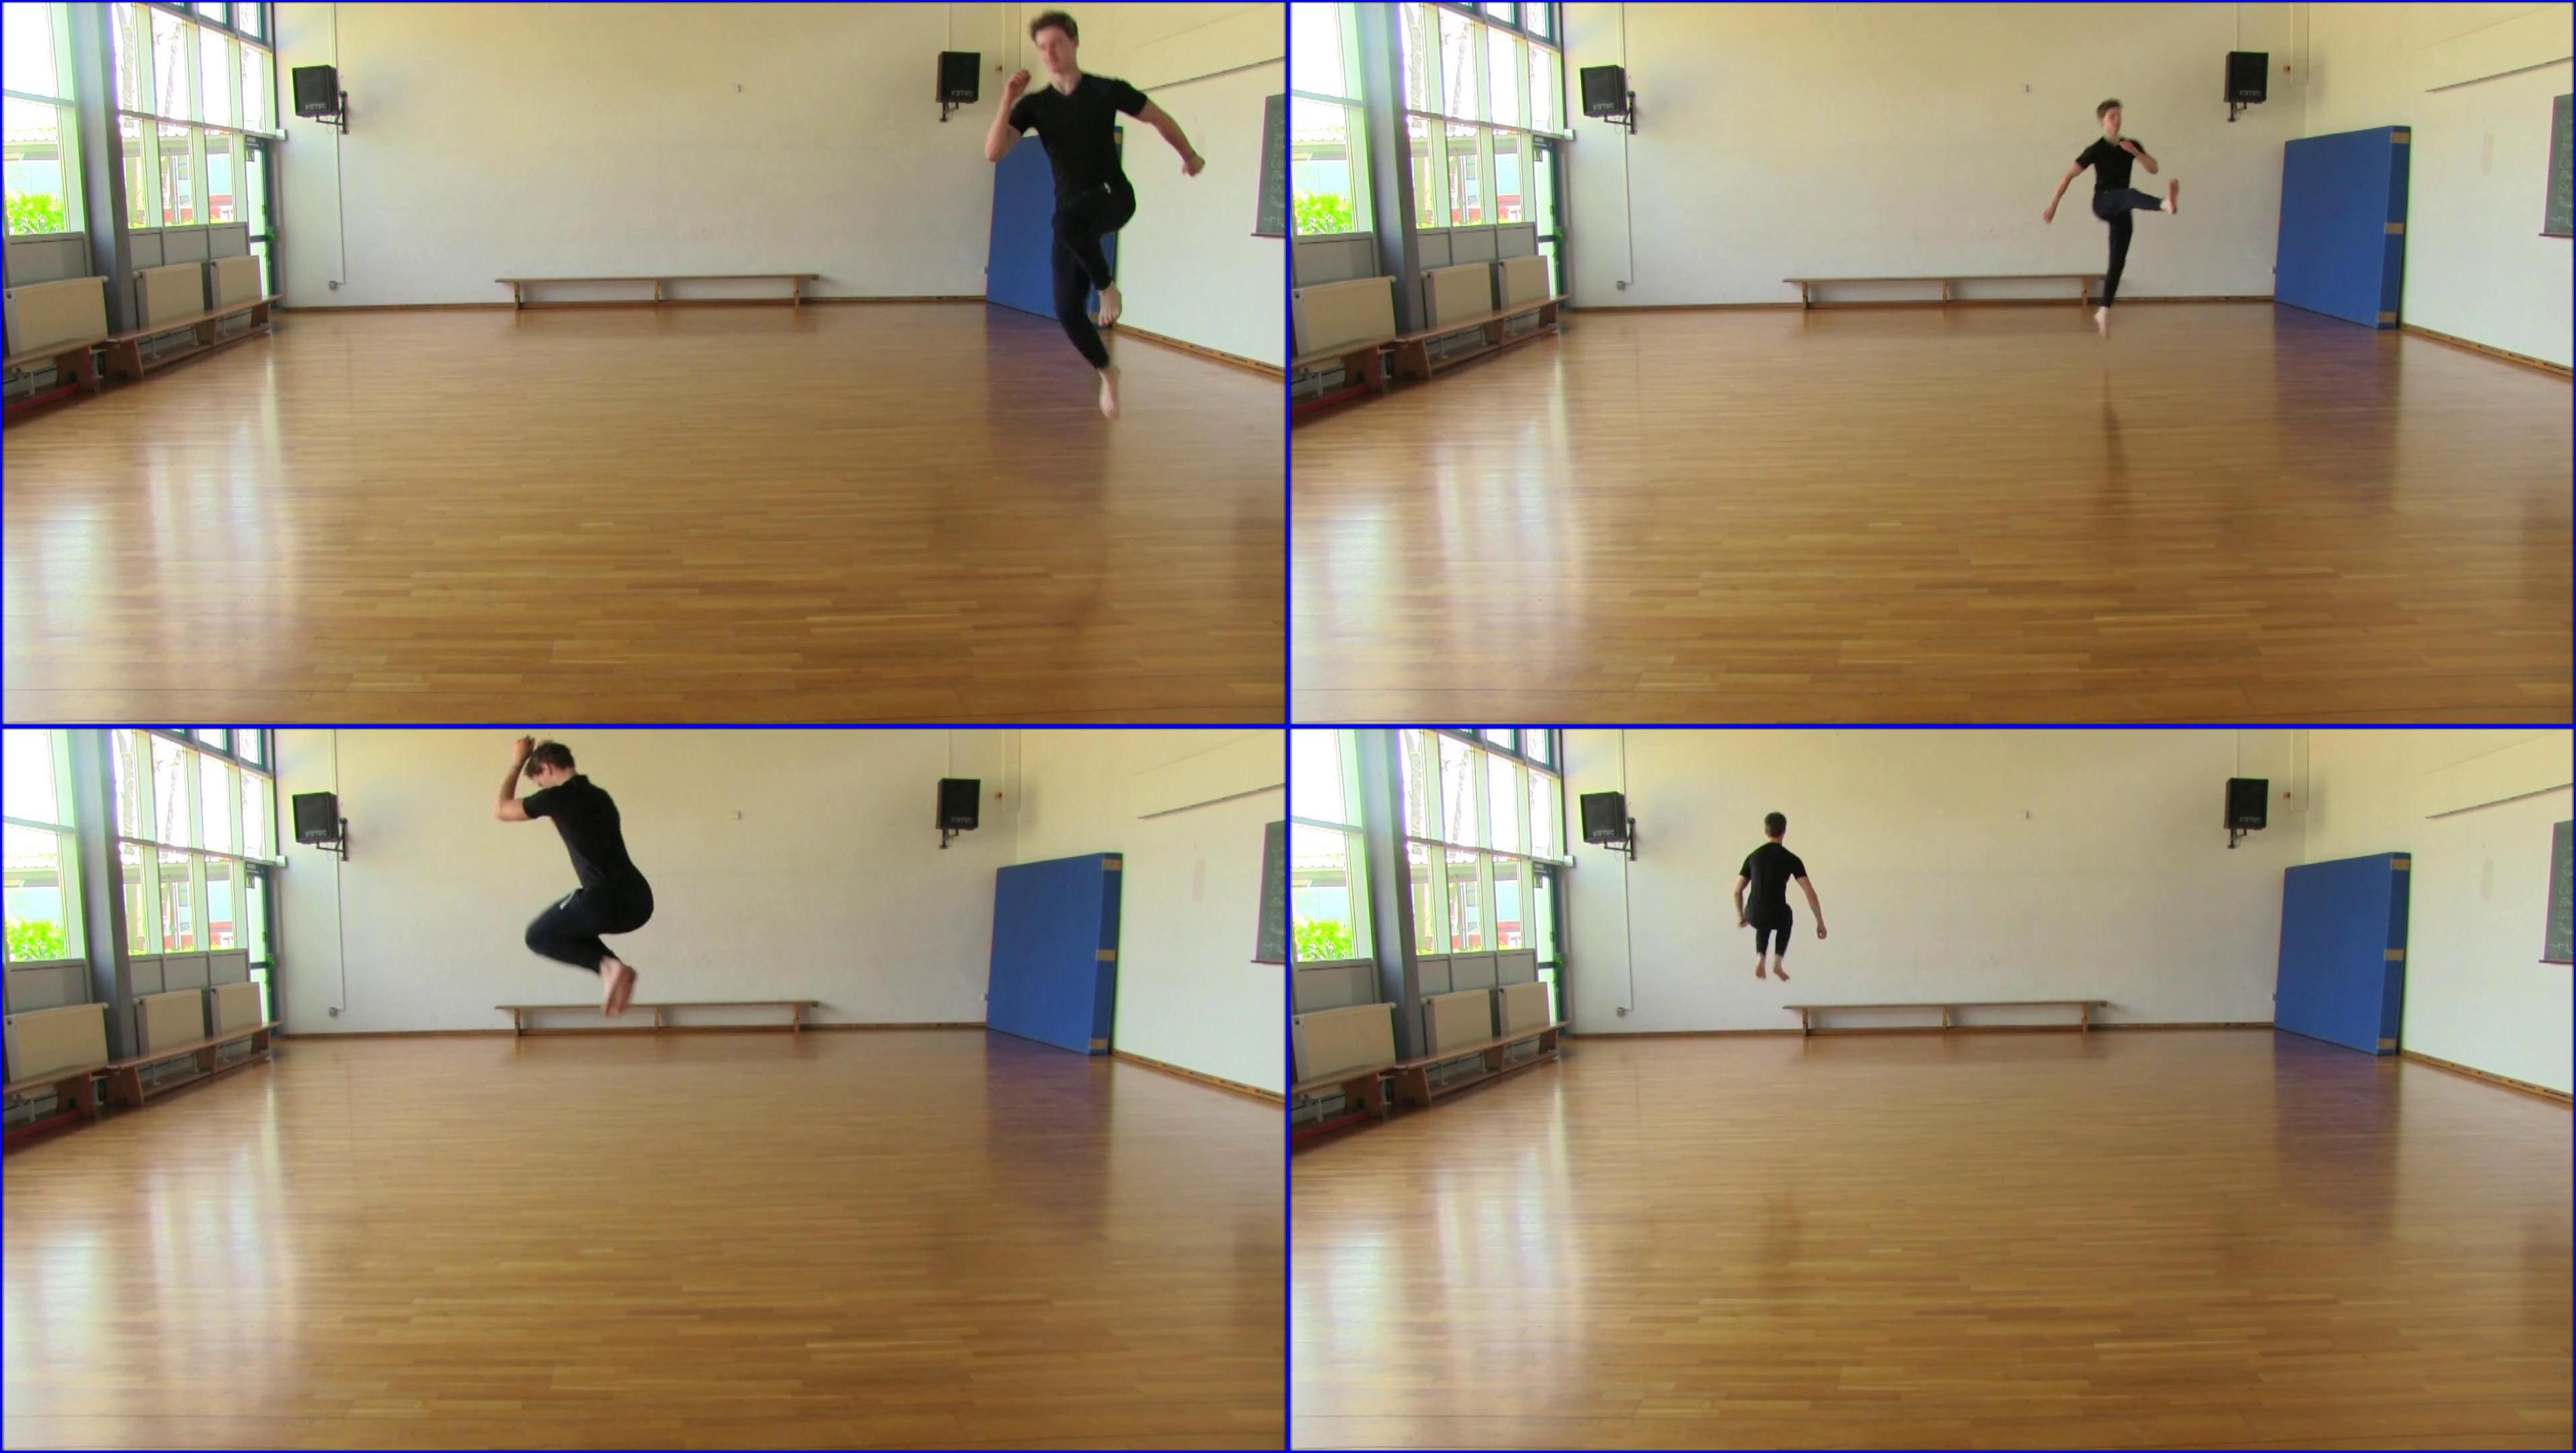
\includegraphics[height={240pt}, width={400pt}]{Thesis/images/jump_time_long.jpg}
\caption{An instance of the \textit{jump} task, which has been evaluated as \textit{long} in the \textit{time in air} dimension of the task}
\label{jump_time_long}
\end{figure}

\subsubsection{Data Preprocessing} Neural networks work on raw input data; hence there is no need for any handcrafted feature extraction. In other words, we can feed raw image frames to them. Two datasets were created from the raw videos, one for the nine base- and another for the 42 evaluation annotations of the BAST analysis. For the rest of this work, these two datasets are referred to as \textit{bast-base} and \textit{bast-eval} respectively. Following \cite{kay2017kinetics} each video of a student was split into 10-second clips with the annotation extracted from its corresponding XML file. Moreover, the use of a 5-second sliding window was found to be beneficial for the model's performance. Table \ref{tab:number_of_clips} shows the number of clips extracted from the 98 videos for each of the datasets.

\begin{table}[h!]
  \begin{center}
    \caption{Number of clips for the \textit{bast-base} and \textit{bast-eval} datasets}
    \label{tab:number_of_clips}
    \begin{tabular}{l|c|r}
      \textbf{Dataset} & \textbf{\#Clips}\\
      \hline
      bast-base & 3894\\
      bast-eval & 4112\\
    \end{tabular}
  \end{center}
\end{table}

\noindent One thing to note is that the number of clips between the two datasets is pretty close. However, the \textit{bast-eval} dataset has many overlapping annotations and is expected to have many more clips. For example, for a 30 second \textit{spin} clip, using a sliding window of 5 seconds, we can extract 5 clips for the \textit{bast-base} dataset but because the \textit{bast-eval} dataset has three evaluations associated with spinning, namely \textit{spin-flow}, \textit{spin-acceleration} and \textit{spin-continuity} we should be able to extract 15 clips. In the end, the expected size of the \textit{bast-eval} dataset should be about three times as much as the size of the \textit{bast-base} dataset. Unfortunately, this is not the case because only a fraction of the 98 videos dataset was evaluated by certified professionals. Therefore, in the end, the number of clips of the \textit{bast-eval} dataset is much lower than the initial expectations. While this amount of clips is sufficient for the nine base annotations, it is not sufficient for the 42 annotations of the \textit{bast-eval} dataset. This issue is further discussed in Section \ref{insufficient_data}.

\subsubsection{Dataset Split} 

This thesis uses the hold-out method to split the datasets \cite{yadav2016analysis} into three independent sets:

\begin{enumerate}
    \item The training set contains clips that are only used for learning.
    \item The validation set contains clips that are used to assess the classifier's performance during the training phase.
    \item The testing set contains clips that the model has not seen in training or validation and is used for further validating the model.
\end{enumerate}

\noindent After training and validating, the model is also tested on a completely new and unseen before test-set. This ensures a robust validation process given that we have a small dataset and risk overfitting for this very reason. The three splits, training, validation, and testing, were formed by assigning each video to one particular set only. This ensures that we properly separate the sets and do not use clips of the same person for training and testing. $70\%$ of the videos were used for training and $15\%$ for validating and testing, respectively. One disadvantage of using this method is the possible variance of the dataset. Given a random split of videos, the evaluation might be influenced by which videos end up in which set. For this purpose, few random splits were initially performed and used to train various models, all of whom reported roughly similar results. This demonstrated that the dataset has little variance. Therefore, in the end, a random split between train and validation was picked, and almost all model trainings were performed with that. For the testing set, different videos were handpicked in order to ensure variety in backgrounds, lightning, and various other conditions.

\subsubsection{Input Modalities} This thesis utilizes three different input modalities for feature extraction by the models: 

\begin{itemize}
    \item RGB: Conventional RGB image frames. For examples regarding different annotations see Figures \ref{bast_contract_expand} and \ref{jump_time_long}.
    \item Optical Flow: A method discussed in Section \ref{background_optical_flow} that detects changes on a pixel level between consecutive frames. For an example see Figure \ref{flow_swing_figure}.
    \item Skeleton data: formed by stacking 17 key points thorough the human body. For an example see Figures \ref{walk_heatmap} and \ref{rotate_pose}.
\end{itemize}

\bigskip
\noindent Using different input modalities ensures more robust models as well as models with a better performance. Indeed, when compared to the \textit{RGB} input flow modality, the \textit{optical flow} modality specialises in picking up movements, while the \textit{pose} modality remains unaffected by the background variations. In this work, the first two modalities, namely \textit{RGB} and \textit{optical flow} were merged together to form two-stream models. It is also possible to merge the \textit{RGB} and \textit{skeleton} modalities through late fusion, although this was not explored in this thesis. In a production setting, we could, therefore, merge all three of these input modalities. Moreover, future research in the BAST analysis is encouraged to test out such models.

\subsubsection{Skeleton Dataset}

\begin{figure}[h]
\center
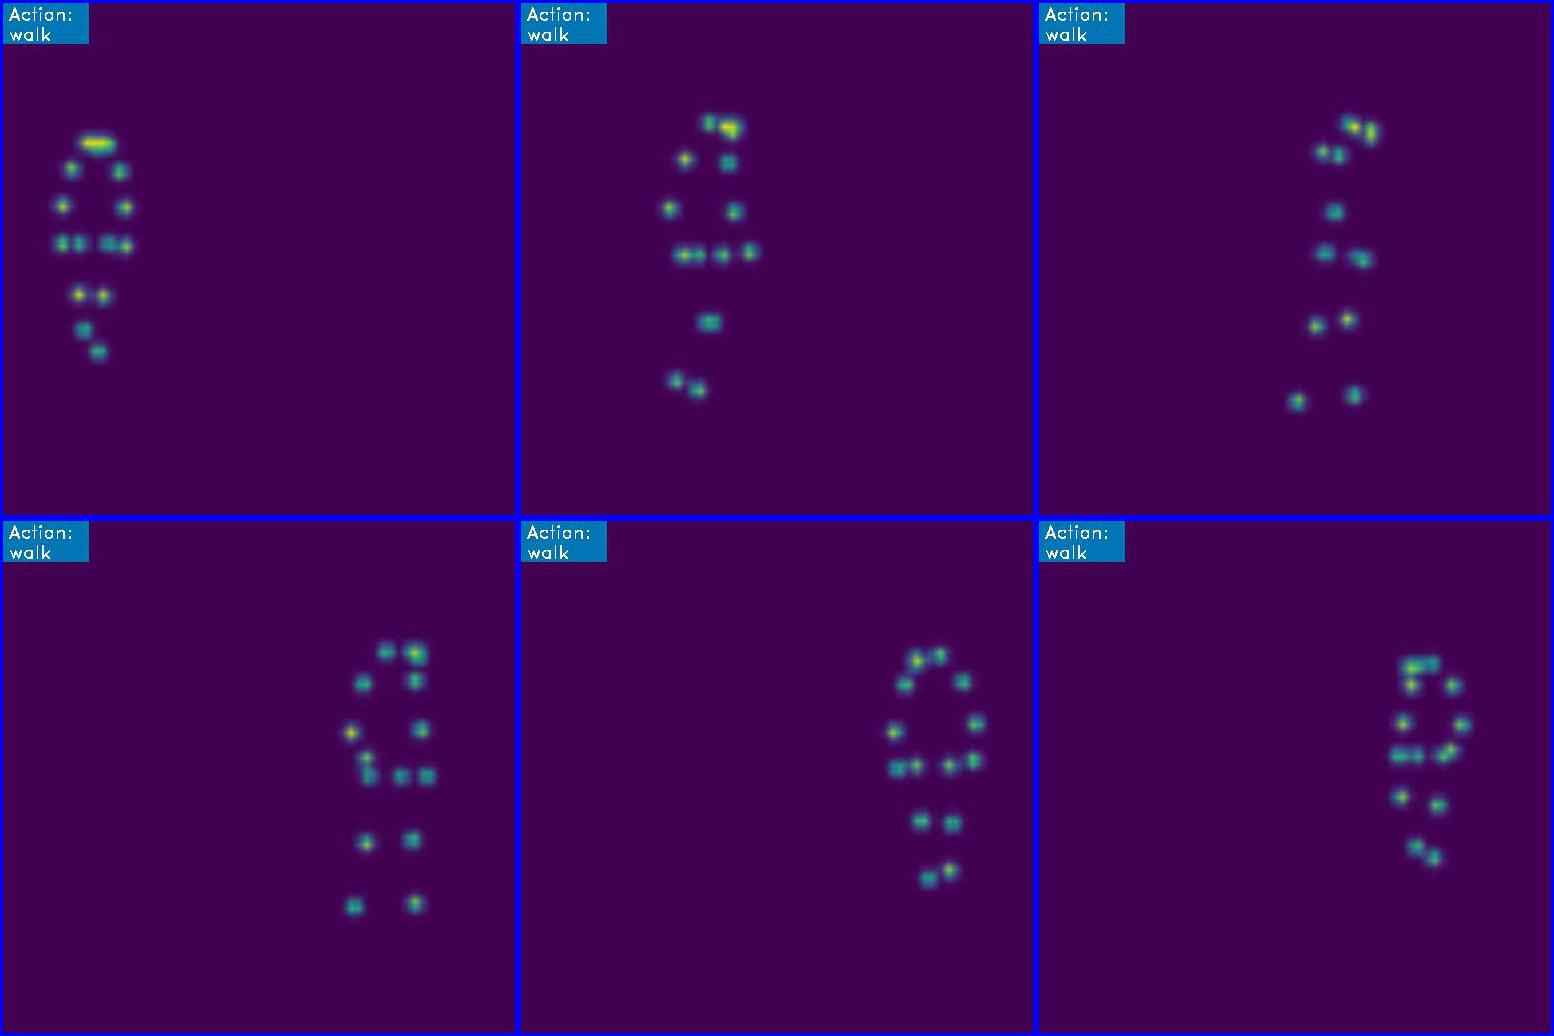
\includegraphics[height={240pt}, width={370pt}]{Thesis/images/walk_heatmap.jpg}
\caption{2D heatmaps formed by the 17 coco keypoints for the \textit{walk} task}
\label{walk_heatmap}
\end{figure}

\noindent In order to extract skeleton data from the videos, a top-down approach was used. The task is divided into two stages. Initially, person detection is performed on the frame using a pre-trained Faster-RCNN model \cite{ren2015faster} with a resnet50 back-bone and a detection threshold of $0.5$. Afterward, given human bounding boxes, single-person pose estimation is performed. For pose estimation, HRnet \cite{wang2020deep} trained on the COCO keypoints \cite{lin2014microsoft} is used.

\bigskip
\noindent The format of PoseC3D annotations is as follows. The complete dataset is serialized and stored in a single python pickle file, for example, \textit{bast-base-train.pkl} for the training set of the \textit{bast-base} dataset. This file is a list of length 2591, with each item being a dictionary representing the skeleton annotation of one clip in the training set. Each dictionary has the following fields:

\begin{itemize}
    \item keypoints: the 17 keypoint coordinates in the x-y coordinate system that are stored in an array of shape: \textit{\#people $\times$ temporal length (of clip) $\times$ 17 keypoints (coco keypoints) $\times$ 2 (x, y coordinates)}.
    \item keypoints' score: the confidence that the model has on these keypoints that are stored in an array of shape: \textit{\#people $\times$ temporal length $\times$ \#keypoints}.
    \item frame directory: corresponding video name.
    \item label: the corresponding action category.
    \item image shape: the image shape of each frame.
    \item total frames: the temporal length of the clip.
\end{itemize}

\noindent The 17 COCO keypoint coordinates correspond to: \textit{0: nose}, \textit{1: left eye}, \textit{2: right eye}, \textit{3: left ear},  \textit{4: right ear}, \textit{5: left shoulder}, \textit{6: right shoulder}, \textit{7: left elbow}, \textit{8: right elbow}, \textit{9: left wrist}, \textit{10: right wrist}, \textit{11: left hip}, \textit{12: right hip}, \textit{13: left knee}, \textit{14: right knee}, \textit{15: left ankle}, \textit{16: right ankle}. They cover all of the human body and its parts, which is especially useful for capturing the fine-grained actions of the \textit{bast-eval} task.

\bigskip
\noindent In total, for the \textit{bast-base} dataset there were 3879 extracted such dictionaries. The accuracy of the two-stage top-down skeleton extraction process is almost perfect, namely $99.6\%$. Figure \ref{walk_heatmap} shows the keypoint heatmap volume visualization for the \textit{walk} task, while Figure \ref{rotate_pose} shows the pose estimation results for the \textit{rotate} task. As we can see, utilizing the human skeleton enables the model to solely focus on the performed action at hand, and the influence of external factors such as background variation is solved. The utilized pose human action recognition model in this thesis is PoseC3D. Results with this model are presented in Sections \ref{research_question_1} and \ref{research_question_2} for the \textit{bast-base} and \textit{bast-eval} datasets respectively.

\bigskip
\begin{figure}[h]
\center
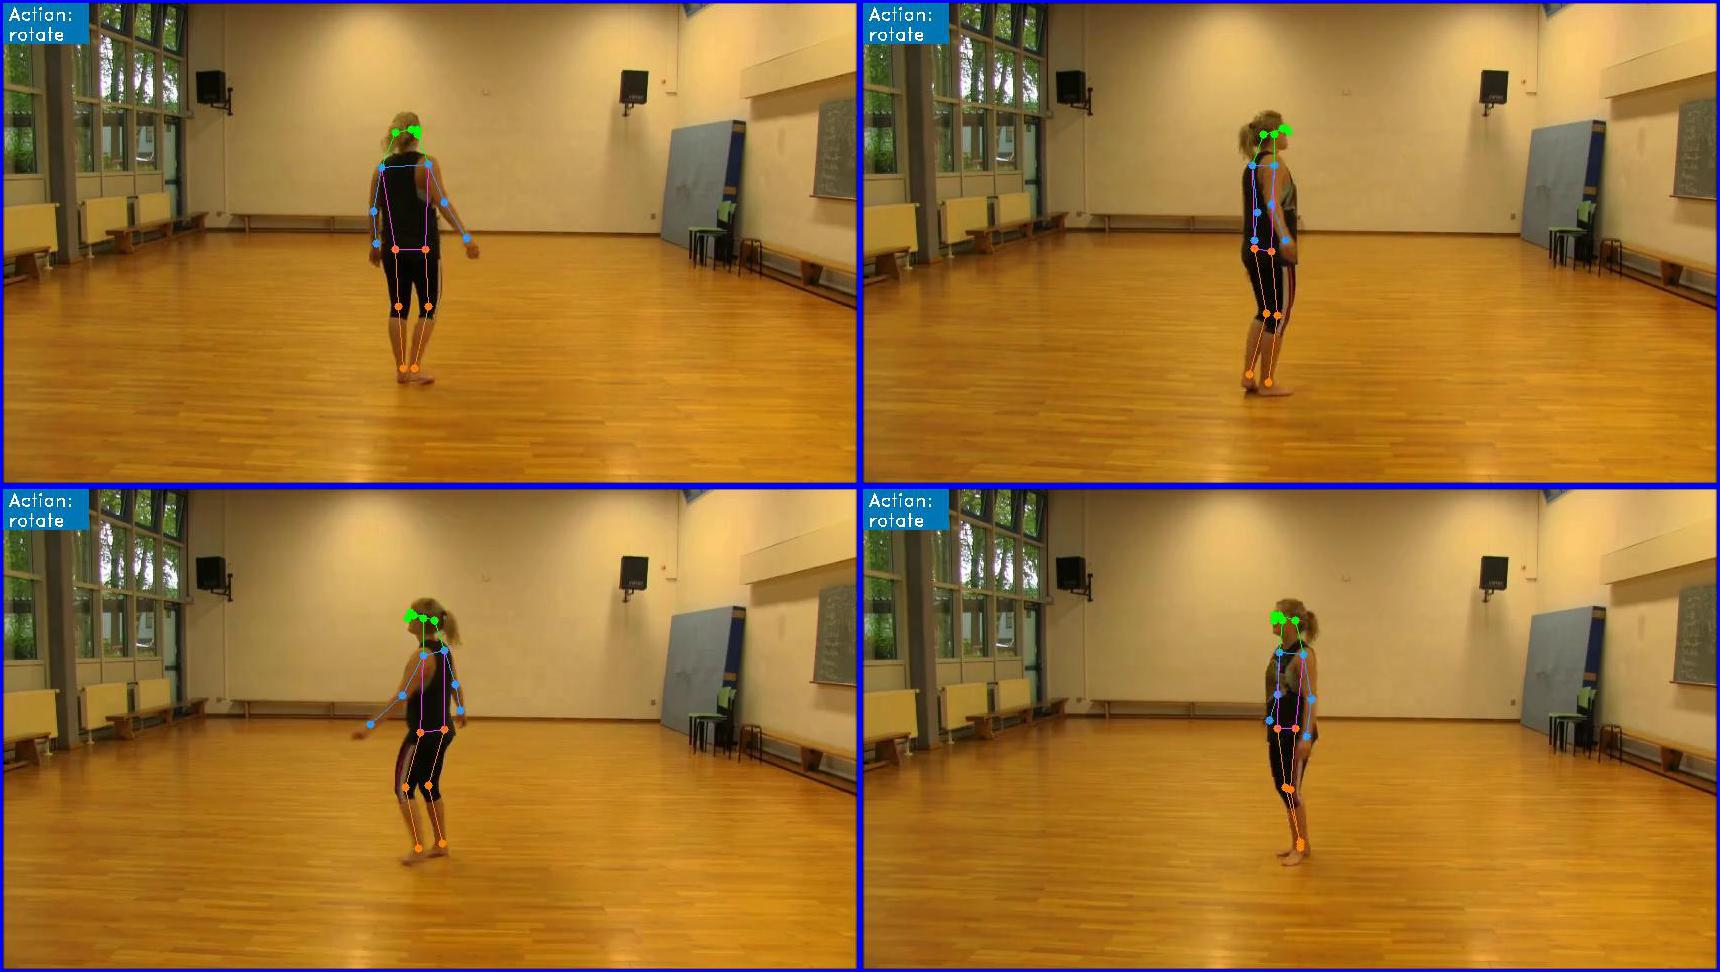
\includegraphics[height={230pt}, width={370pt}]{Thesis/images/rotate_pose.jpg}
\caption{Pose estimation for the \textit{rotate} task}
\label{rotate_pose}
\end{figure}

\newpage
\subsection{Domain Testing Datasets}
\label{domain_testing_dataset}
In order to test the capabilities and robustness of the trained models to extrapolate to third domains, in the context of the \textit{Vortanz} project, two additional datasets were utilized. The datasets consist of different types of movements as well as different qualities of these movements. Hence it is expected that it will be hard for the models to generalize in these new domains. The two datasets are listed below:

\begin{itemize}
    \item \textit{bast-avatar} is the dataset that consists of videos from the second task of the BAST analysis. The participants were asked to emulate \textit{water}, \textit{fire}, \textit{air}, \textit{earth} using their body movements. Each task lasted about one minute. As the subjects are given free reigns in the performance, the variety of movements presented in this dataset is enormous. Some participants also performed dance-like movements. Therefore, this study considers this dataset domain testing because of this variety, although it is not such a dataset strictly speaking.
    
    \item \textit{kinesphere} is a dataset that consists of videos where the participants perform the kinesphere movement on three different levels: \textit{narrow-kinesphere}, \textit{middle-kinesphere}, and \textit{wide-kinesphere}. This dataset was recorded by professional dancers and hence belongs to a pure dancing domain. Its movements are very fine-grained (even more so than the \textit{bast-eval} dataset itself) and are expected to be complex to recognize for the A.I. models.
\end{itemize}

\noindent Figure \ref{kinesphere_dataset} illustrates a movement from the \textit{kinesphere} dataset, and Figure \ref{bast_avatar} illustrates a movement from the \textit{bast-avatar} dataset. In the latter, two people are illustrated. The first one is trying to imitate a swimming position, while the second is trying to imitate a wave pattern with his hand.

\begin{figure}[h]
\center
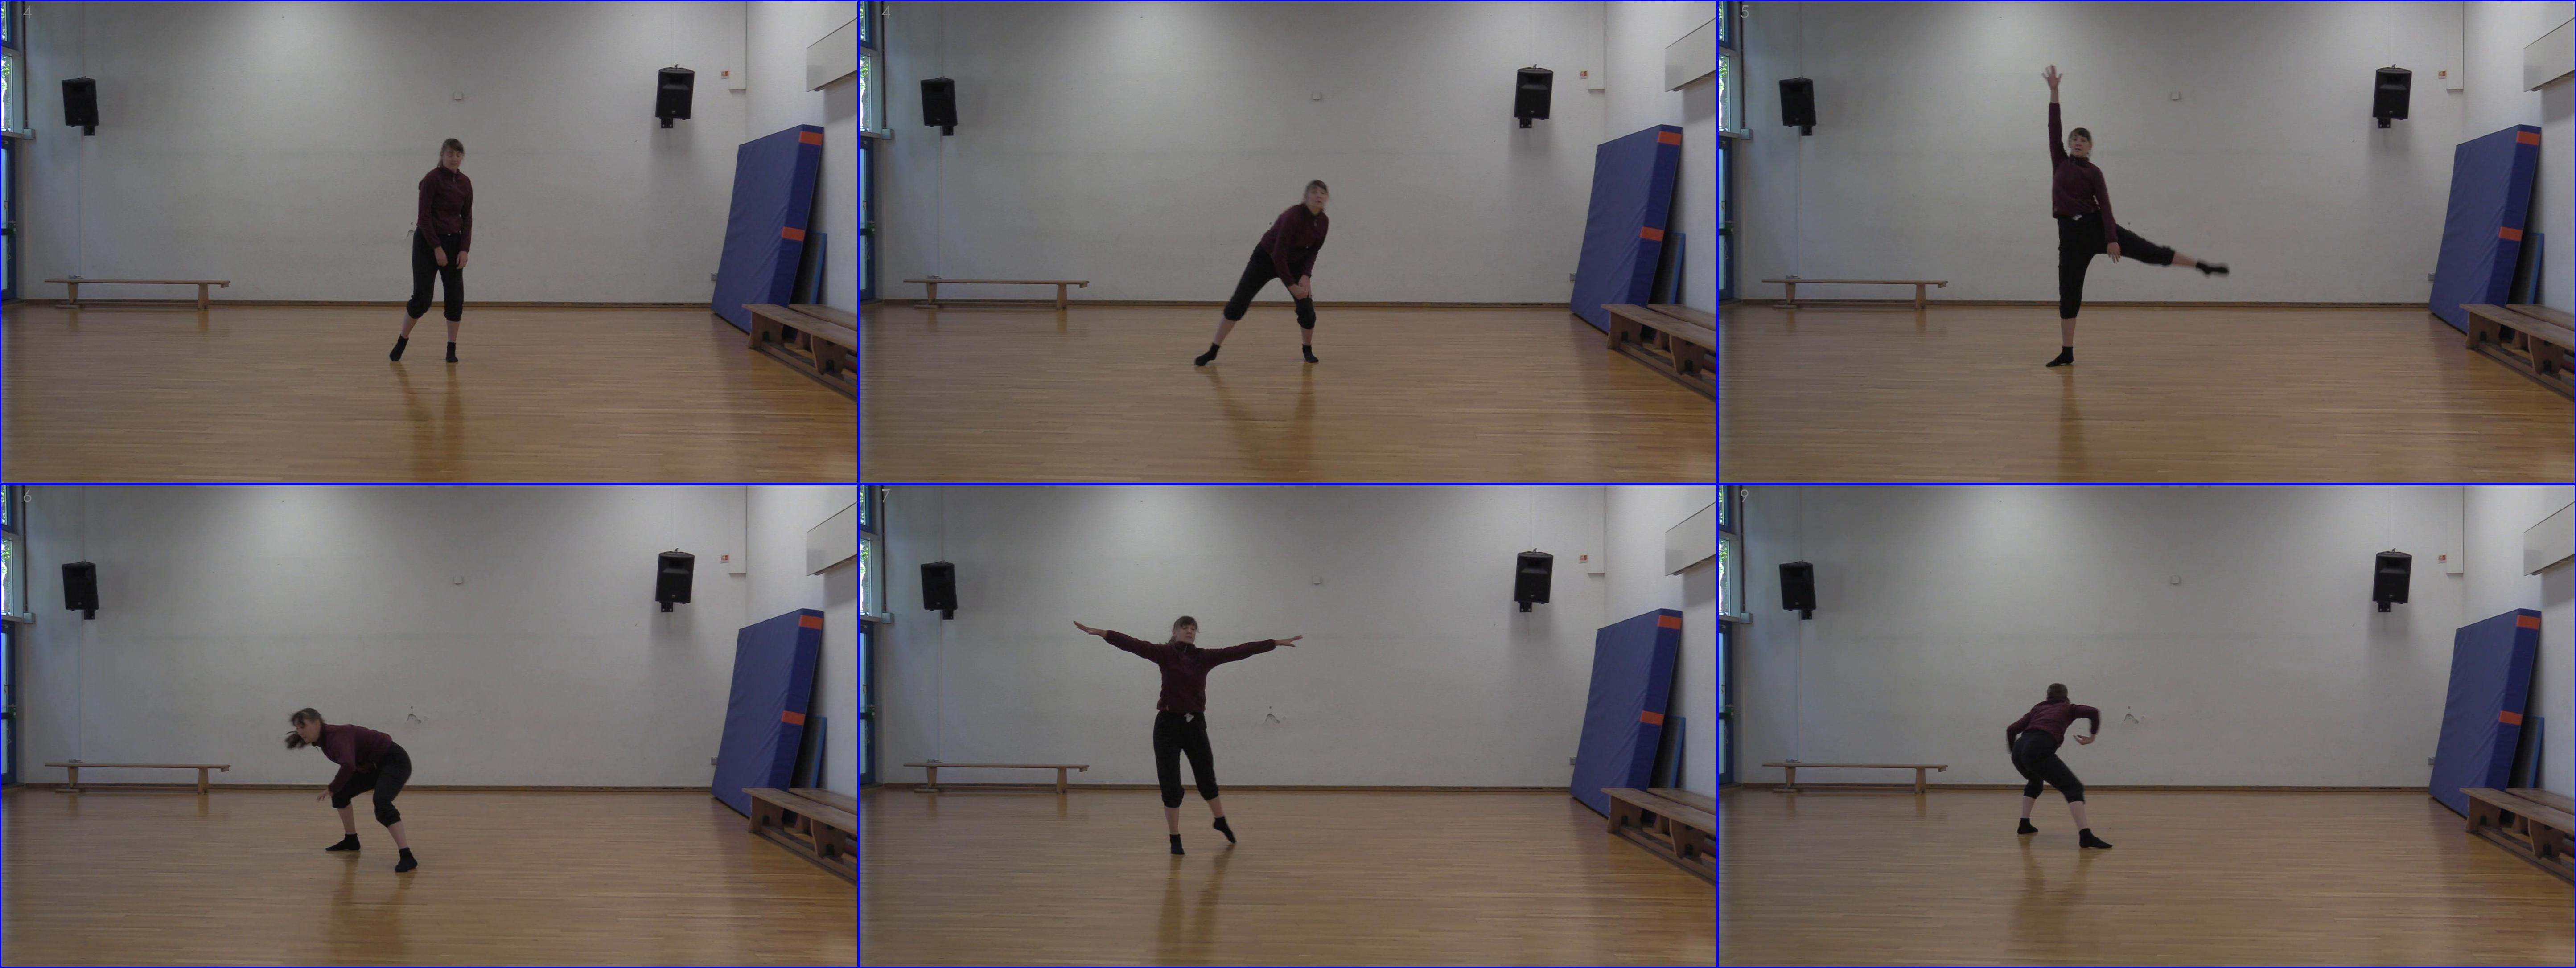
\includegraphics[height={210pt}, width={380pt}]{Thesis/images/kinesphere.jpg}
\caption{Kinesphere movement from the \textit{kinesphere} test dataset}
\label{kinesphere_dataset}
\end{figure}

\begin{figure}[h]
\center
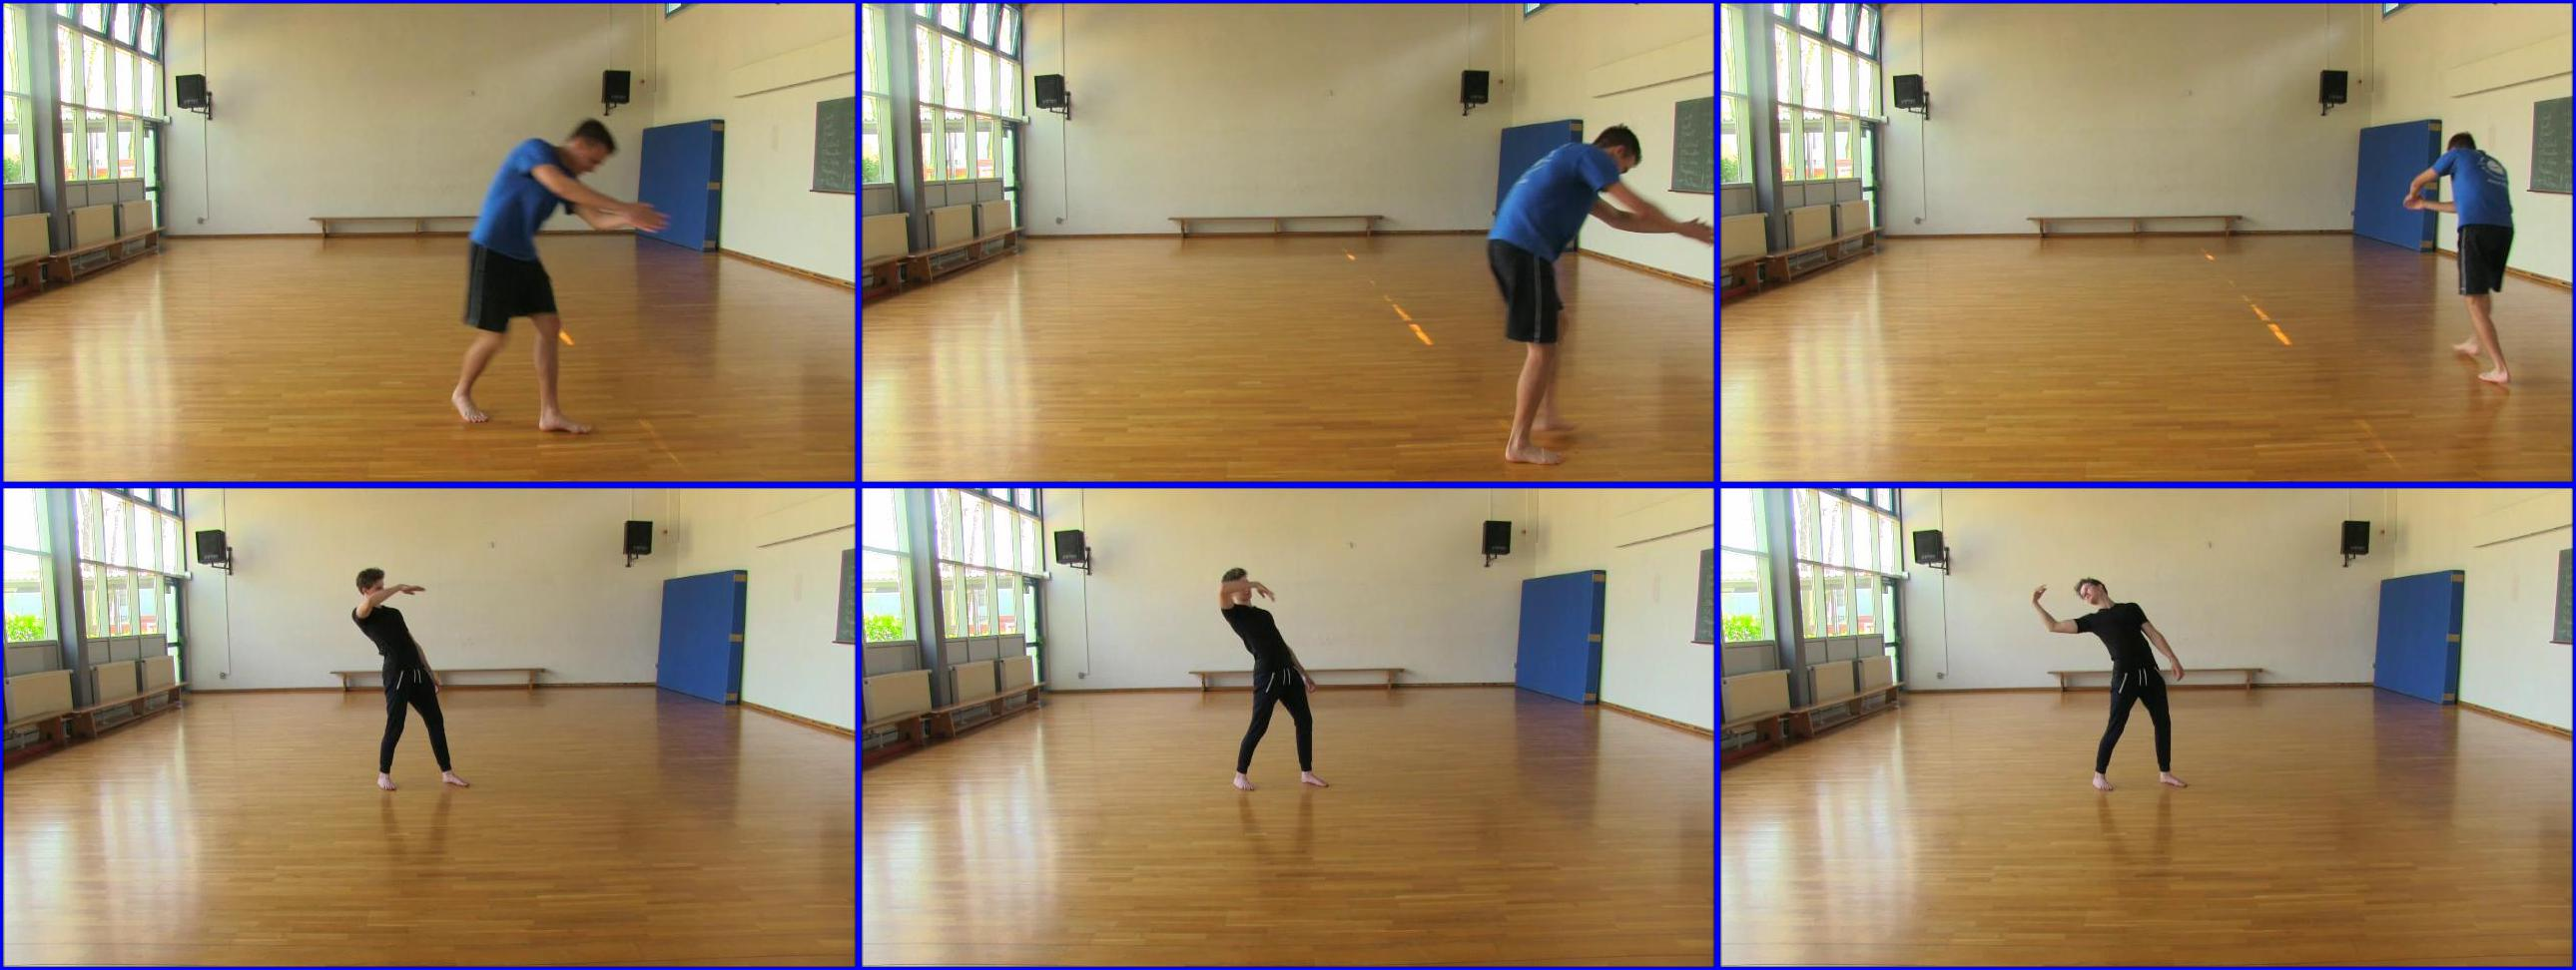
\includegraphics[height={210pt}, width={380pt}]{Thesis/images/bast_avatar.jpg}
\caption{Emulation of \textit{water} using body movements from the \textit{bast-avatar} test dataset}
\label{bast_avatar}
\end{figure}
\newpage

\subsection{Benchmark Datasets}
\label{benchmark_datasets}
As already discussed in chapter \ref{convolutional_neural_networks_background}, ConvNets are the current state-of-the-art algorithms in the domain of human action recognition. However, the crucial requirement to develop a HAR system using deep learning is to use appropriate human action datasets. These datasets should be sufficiently rich in the variety of human action that they capture as well as big enough for the deep learning architecture to learn. Indeed, these two properties are a prerequisite for any dataset before it is used for training any deep learning architectures, and the bigger a dataset is, and the more variety it has, the better are the results that are obtained. 

The variety and size of the BAST dataset are enough for forming the \textit{bast-base} dataset. However, the same cannot be said about the \textit{bast-eval} dataset (see Section \ref{insufficient_data}). Therefore, a principal strategy that was used in this thesis to solve this problem was to use weights of models pre-trained from important benchmark datasets in the field. Transfer learning is a commonly used strategy in deep learning to solve the problem of insufficient training data \cite{tan2018survey}. Using such pre-trained models on other domains has been shown to significantly improve the performance in the domain under inspection. In the field of HAR, \cite{carreira2017quo} was the first one to demonstrate the gains in performance and robustness when pre-training with datasets such as ImageNet or Kinetics. Omni-Sourced \cite{duan2020omni} another dataset created for pre-training purposes has also been shown to improve the model's performance and robustness by quite a bit. The effect of transfer learning are studied in details at Section \ref{research_question_4}. Below we take a look at the datasets that were utilized for pre-training in the context of this work.

\subsubsection{Kinetics}
\label{kinetics400}
The first version of the Kinetics dataset \cite{kay2017kinetics} contains 400 human action classes with at least 400 video clips for each action. Each clip lasts at least 10 seconds and was taken from youtube videos in order to ensure variety in the dataset. Currently, it is the dominating benchmark dataset for HAR. Since then, there have been two more versions, namely, Kinetics-600 \cite{carreira2018short}, and Kinetics-700 \cite{carreira2019short} which expanded the number of classes to 600 and 700 respectively. The classes include human-object interaction, such as \textit{playing chess}, human-human interactions such as \textit{shaking hands} or single human actions such as \textit{shaking head}. The dataset also contains dancing actions such as \textit{belly dancing} or \textit{salsa dancing}. Figure \ref{kinetics_sample} shows four actions from the Kinetics dataset. Because the Kinetics dataset is so huge, that is has actions that cover a variety of domains, it has been demonstrated that pre-training the models by it, does improve the performance in the domain under inspection \cite{carreira2017quo}. Indeed, for the \textit{bast-base} dataset, pre-training on Kinetics improved the performance by quite a bit. 

\begin{figure}[h]
\center
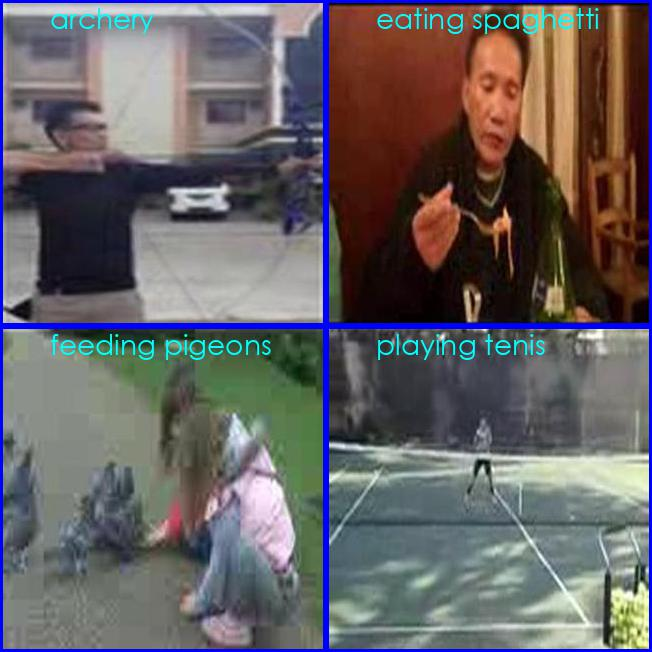
\includegraphics[height={160pt}, width={200pt}]{Thesis/images/kinetics_sample.jpg}
\caption{Four action samples from the Kinetics-400 dataset \cite{kay2017kinetics}}
\label{kinetics_sample}
\end{figure}

\subsubsection{FineGym}
\label{fine_gym}
FineGym is a dataset that is quite different from the others in that it focuses on capturing deeply fine-grained actions in the domain of gymnastics such as \textit{switch leap with 0.5 turn}\footnote{Example --- \url{https://www.fig-aerobic.com/C-425-SWITCH-SPLIT-LEAP-TURN_a907.html}} \cite{shao2020finegym}. This is in contrast to previous datasets, which are mostly crowd-sourced and focus on coarse-grained actions such as \textit{eating spaghetti} or \textit{playing tennis} from Kinetics. On the contrary, the differences between the actions of FineGym are quite subtle, can be very fast-paced, involve extreme body poses, and are only obtained with the help of expert knowledge. FineGym provides temporal annotations at both action and sub-action levels with a semantic hierarchy. Thus \textit{a balance beam} event is further divided into a sequence of sub-elementary actions such as \textit{leap-jump-hop}, \textit{beam-turns}, \textit{flight-salto}, \textit{flight-handspring} and finally \textit{dismount}. The idea behind assembling FineGym is that architectures that achieve good results on such a complex dataset might also result in useful models in real-world applications, which require the capabilities of parsing an activity into phases and differentiating between subtly different actions such as sports analysis. Current state-of-the-art models usually work well on datasets with coarse-grained actions, but this frequently offers difficulties when these architectures are utilized in real-world scenarios because the models do not work quite as well as they had worked on the benchmark datasets. Incidentally, this is also the case with the \textit{bast-eval} dataset, which consists of rather fine-grained actions when compared to the more straightforward \textit{bast-base} dataset. A pre-training with the FineGym dataset could potentially help the model's performance as opposed to pre-training with conventional datasets such as Kinetics. Indeed the FineGym paper shows that pre-training on datasets that target coarse-grained action recognition is not always beneficial for fine-grained action recognition tasks.

\subsubsection{Omni-Sourced}
\label{omni-sourced}
A dataset that is formed by crawling and scraping raw data on the web in different formats such as images, trimmed or untrimmed videos\cite{duan2020omni}. In order to find the raw data, class labels are used as keywords on search engines, different social media, and video sharing platforms. This data is then filtered out using a so-called teacher network, which has already been pre-trained to detect the desired classes. This removes irrelevant samples with low confidence from the dataset since web data is extremely noisy. After that, different transformations are applied that convert each type of web data to the target input format. For example, still images are transformed via homographic transformations to pseudo-videos. The end result is a dataset that is rich in its variety and with very little noise. Models pre-trained on the omni-sourced dataset showed improved accuracy, even more so than those pre-trained on the kinetics dataset, and set the new state-of-the-art in several other benchmark datasets. This serves to further stress the importance of transfer learning in human action recognition.

\subsubsection{Other}
\label{other}

\noindent\textbf{Something-Something}: The something-something dataset focuses on common sense reasoning and fine-grained actions \cite{Goyal_2017_ICCV}. Similar to FineGym, the hope is to develop architectures can pick up detailed physical aspects of actions and scenes. For example, it might be relatively more straightforward for the model to learn the actions in Figure \ref{kinetics_sample} when compared to more subtle actions such as \textit{picking something up}, \textit{dropping something into something} or \textit{pushing something so that it spins}, which generalize the \textit{something} part into a wide range of objects. This dataset could also provide useful weights for the \textit{bast-eval} task.

\bigskip
\noindent\textbf{NTU}: The NTU dataset has two versions, one with 60 actions \cite{shahroudy2016ntu}, and the other with 120 \cite{liu2019ntu}. It provides four different modalities of data for each sample, RGB, depth, 3D skeletons, and infrared. In the context of this work, only pre-training with the first modality was utilized. It contains different actions in daily life or health-related ones such as \textit{taking a selfie}, \textit{make a phone call} or \textit{nausea or vomiting condition}.

\bigskip
\noindent\textbf{Diving-48}: Another fine-grained action dataset, whose focus is the diving domain \cite{li2018resound}. It contains numerous clips for 48 specific dive sequences. Similar to FineGym and Something-Something, the hope is to aid the development of HAR architectures for fine-grained actions, specifically long-term temporal dynamics.

\bigskip
\noindent\textbf{Ufc}: One of the earliest benchmark datasets used for deep learning, the \textit{Ufc101} dataset contains 101 human actions covering a wide range of activities, some of which are depicted in Figure \ref{ufc_actions} \cite{soomro2012ucf101}.

\bigskip
\noindent\textbf{Hmdb}: Another early benchmark dataset in the field containing about 51 actions similar to \textit{Ufc} \cite{kuehne2011hmdb}.

\newpage
\subsection{Deep Learning Pipeline}
\label{dl_pipeline}
While deep learning architectures extract features directly from raw data, the implementation of various data augmentation techniques or hyperparameter tuning of various model and run time settings have been shown to improve model performance and robustness drastically. Indeed, the deep learning pipeline is perhaps as important as the architecture of the model being used. All the following implementations were realized using the MMAction2 framework \cite{2020mmaction2}. This section describes the complete pipeline for running the model training experiments and gives two examples regarding the implementation of the model's architecture and the use of its hyperparamters.

\subsubsection{Pre-processing Pipeline}

The two main pre-processing pipelines that are worth to discuss in this thesis are the video sampling strategy and some of the most important data agumentation techniques that were used.

\bigskip

\noindent\textbf{Sampling Strategies}: Two frame sampling strategies have been utilized: Dense and Uniform sampling. The former is the de-facto used strategy for 3D ConvNets and the later for the 2D ones. These sampling strategies are applied to the input frames extracted on the fly from the videos. The sample strategy is defined as $clip\_length \times frame\_interval \times num\_clips$.

\bigskip
\noindent Dense sampling samples continuous frames. More specifically, it samples one frame every $frame\_interval$ frames until it gets $clip\_length$ frames. For example, if we use a $32 \times 2 \times 1$ sampling strategy and supposing a clip of 104 frames ($[0:103]$), dense sampling might select frames $0, 2, 4, ..., 64$.

\bigskip
\noindent On the other hand, uniform sampling samples, have a  $clip\_length = 1$, divide all frames into $num\_clips$ parts and sample one frame from each part. For example, a uniform sampling strategy of $1 \times 1 \times 8$ would divide the 104 frames into 8 groups $[0, 12], [13, 26], ..., [91, 103]$ and pick one frame from them, like so: $0, 13, ..., 91$.

\bigskip
\noindent\textbf{Data Augmentation}: Is a widely used technique in image and video processing employed to generate diverse training samples and prevent overfitting by inserting some degree of bias into the dataset \cite{mikolajczyk2018data}. The immediate consequence of this is that it enables the model to better generalize for future samples. The second most important quality of data augmentation is that it provides the deep learning models with more sorely needed data, which further boosts the model's performance. This thesis exploits several data augmentation techniques, the most important of which are listed below:

\begin{itemize}
    \item Resize: all images are resized in two-stages: first to a size of $256$ and then after cropping them in some way (see below), to a size of $224$.
    \item Multi-scale crop: crops the image with a list of randomly selected scales.
    \item Random-resized crop: a random crop that in addition specifies the area and height-weight ratio range.
    \item Flip: flips the image with a given probability. Reverses the order of elements in the image with a specific direction.
    \item Normalize: the images are normalized with a particular mean and standard deviation value.
\end{itemize}

\subsubsection{Optimization Pipeline}
\textbf{Regularization techniques}: The two main regularization techniques used are the batch normalization (BN) \cite{ioffe2015batch} and dropout \cite{srivastava2014dropout}. BN is an important component used to normalize the activations in intermediate layers of deep neural networks into a standard Gaussian distribution. In other words, it preserves a mean output close to zero with a standard deviation close to one. It has become an established technique that improves the model's accuracy and speeds up the training process. Dropout is another widely used technique to reduce the overfitting of neural networks. The idea behind it is to drop units and their connections during the training process randomly. This makes the network more robust for future unseen samples. It has been shown to improve the performance of neural networks in all kinds of domains such as object classification, digit recognition, and speech recognition. Both of these techniques are duly employed in this thesis work.

\bigskip
\noindent\textbf{Optimizer}: For all experiments, the optimizer used was stochastic gradient descent (SGD), also known as gradient descent with momentum \cite{sutskever2013importance}. The current human action recognition literature indicates that this is the best optimizer to use, generally speaking. The learning rate of the optimizer was determined according to the linear scaling rule \cite{goyal2017accurate}. This means that the learning rate is proportionate to the number of GPUs utilized for training and the number of videos passed to a GPU for processing. For example, if 4 GPUs $\times$ 2 videos per GPU are used then $lr = 0.01$; if 16 GPUs $\times$ 4 videos per GPU are used then $lr = 0.08$.

\subsubsection{Model Settings}
The models' settings (parameters and hyperparameters) were all picked according to the respective paper's recommendations (see Section \ref{literature_review} for a general review) but also common best practices of the computer vision community, an in particular of the MMAction2 codebase. Below, two samples are given in order to give a general impression. For the specific details, the source code, available on GitHub, should be consulted. 

\bigskip
\noindent The first example below, represents the settings of the SlowFast model. The model is composed of two parts: the backbone, responsible for extracting the features, and the head which is responsible for the final classification. The backbone uses a modified version of 3D ResNets with a $resample\_rate$, $speed\_ratio$ and $channel\_ratio$ of $8$. The Slow and Fast pathways, which are $50$ layers deep, are then constructed with their respective kernels, pools, and dilations as specified in the paper. The head of the model, which performs the final classification, has $2304$ total input channels, where $2048$ account for the Slow pathway and only $256$ for the lighter Fast pathway. Average pooling is used and a dropout ratio of $0.5$ by default. Finally there are $9$ output classes when considering the \textit{bast-base} task.

\vspace{5mm}
\begin{lstlisting}[language=Python, label={listing_slowfast_model}, caption={SlowFast model settings}]

model = dict(
    type='Recognizer3D',
    backbone=dict(
        type='ResNet3dSlowFast',
        pretrained=None,
        resample_rate=8,  # tau
        speed_ratio=8,  # alpha
        channel_ratio=8,  # beta_inv
        slow_pathway=dict(
            type='resnet3d',
            depth=50,
            pretrained=None,
            lateral=True,
            conv1_kernel=(1, 7, 7),
            dilations=(1, 1, 1, 1),
            conv1_stride_t=1,
            pool1_stride_t=1,
            inflate=(0, 0, 1, 1),
            norm_eval=False),
        fast_pathway=dict(
            type='resnet3d',
            depth=50,
            pretrained=None,
            lateral=False,
            base_channels=8,
            conv1_kernel=(5, 7, 7),
            conv1_stride_t=1,
            pool1_stride_t=1,
            norm_eval=False)),
    cls_head=dict(
        type='SlowFastHead',
        in_channels=2304,  # 2048+256
        num_classes=9,
        spatial_type='avg',
        dropout_ratio=0.5),
    # model training and testing settings
    train_cfg=None,
    test_cfg=dict(average_clips='prob'))

\end{lstlisting}
\vspace{5mm}

\bigskip \bigksip
\noindent The second example, represents the settings for the \textit{PoseC3D-SlowOnly} model. Like the above architecture, it is a 3D ConvNet. Its backbone comes from the Slow pathway of the \textit{SlowFast} architecture and is $50$ layers deep. It takes $17$ channels as input, which correspond to the human skeleton consisting of $17$ extracted keypoints of the human body. The restnet backbone has 3 stages and uses a stride and pool size of one for the first layer. For the other layers a spatial stride of $(2, 2, 2)$ a temporal stride of $(1, 1, 2)$ is used. The head is the selfsame head used for the \textit{I3D} model and the number of final classes is $42$ considering the \textit{bast-eval} task. It uses average pooling with a dropout rate of 0.6.

\bigskip \bigskip \bigskip
\vspace{5mm}
\begin{lstlisting}[language=Python, label={listing_slowfast_model}, caption={PoseC3D-SlowOnly model settings}]

model = dict(
    type='Recognizer3D',
    backbone=dict(
        type='ResNet3dSlowOnly',
        depth=50,
        pretrained=None,
        in_channels=17,
        base_channels=32,
        num_stages=3,
        out_indices=(2, ),
        stage_blocks=(4, 6, 3),
        conv1_stride_s=1,
        pool1_stride_s=1,
        inflate=(0, 1, 1),
        spatial_strides=(2, 2, 2),
        temporal_strides=(1, 1, 2),
        dilations=(1, 1, 1)),
    cls_head=dict(
        type='I3DHead',
        in_channels=512,
        num_classes=42,
        spatial_type='avg',
        dropout_ratio=0.6),
    train_cfg=dict(),
    test_cfg=dict(average_clips='prob'))

\end{lstlisting}
\vspace{5mm}

\newpage
\subsection{Interpretability}
\label{interpretability}
Deep Learning models have almost become infamous for their black-box nature \cite{fan2021interpretability}. In other words, studying the structure of a neural network does not give any insights into the structure of the function being approximated by the neural network. The primary motivation for examining the interpretability of the model in this thesis is to examine its weaknesses since interpretability can help identify potential vulnerabilities of a complicated model. For example, a low dropout rate for 3D ConvNet-based architectures might cause the model to overfit the data based on the background. If we can somehow see that the background influences the model, we could pick a higher dropout rate to solve this problem. Alternatively, the dense sampling strategy could ensure a more robust model that picks the subtle difference of the \textit{bast-eval} task better than the uniform sampling strategy does.

\subsubsection{GradCAM}
The method that was utilized in this work to produce visual explanations for decisions of the ConvNet models was Grad-CAM \cite{selvaraju2017grad}. Grad-CAM exploits the gradients of the target concepts flowing into the final convolutional layer to produce a localization map that highlights the critical regions in the image for predicting the concept. These maps are finally overlapped over the input video as heatmaps, which show the image regions that the model most focused on to perform the final classification. The regions that the models trained on the \textit{bast-base} and \textit{bast-eval} datasets based their predictions on are visualized in the final research question at Section \ref{research_question_5}. 

\subsection{Model Evaluation}
\label{model_evaluation}
There are many different ways to evaluate deep learning models. In this thesis, classification accuracy and mean class accuracy have been utilized.

\bigskip
\noindent\textbf{Accuracy}: Is the fraction of predictions that a classification model got right.

\begin{align*}
    Accuracy &= \frac{Number \ of \ correct \ predictions}{Total \ number \ of \ predictions}
\end{align*}

\noindent In particular, we look into the  \textit{top-k} accuracy. \textit{Top-2} accuracy would refer to the accuracy where the ground-truth class matches with any one of the two most probable classes predicted by the model. For the \textit{bast-base} task, we use the \textit{top-2} accuracy because there can be overlaps during the performance of a task. For example, some subjects are performing the \textit{rotate} task while being on tiptoe, which means that they are also performing the \textit{tiptoe} class. Another way to solve this (and perhaps the better way) would be to rather design a multi-label classification problem, which does not consider the classes mutually exclusive. This work, however, follows a multi-class classification problem, which does consider the classes mutually exclusive and hence the reasoning behind the \textit{top-k} accuracy approach.

For the \textit{bast-eval}, on the other hand, task we use a \textit{top-3} accuracy because at most three actions can be performed at the same time. This is the case for the \textit{spin} task for example that be can evaluated on three dimensions, namely \textit{spin-acceleration}, \textit{spin-flow} and \textit{spin-continuity}. One possible such set of evaluations could thus be: \textit{spin-acceleration-none}, \textit{spin-flow-free} and \textit{spin-continuity-single}. Hence we need to take into consideration the \textit{top-3} accuracy.

\bigskip
\noindent\textbf{Mean class accuracy}: Computed by dividing the sum of the dominant diagonal over the sum of all the elements of the confusion matrix between the prediction scores for each class and the ground truth labels. 

\bigskip
\noindent Using the \textit{top-k} accuracy has the disadvantage of favoring those classes that do not have \textit{k} possible, equally valid outcomes. For example, the task \textit{jump} is evaluated only on two dimensions, namely \textit{emphasis} and \textit{time in air} so we should really be looking at the \textit{top-2} accuracy. Looking at the \textit{top-3} accuracy means being more lenient to the model than should be the case. On the other hand, however, considering that the \textit{bast-eval} task has $42$ annotations, this could still be considered a good choice. 

\noindent Hence in the final evaluation of the model's performace, while the priority is given to the \textit{top-k} accuracy, the \textit{mean class accuracy} is also considered.


\newpage
\section{Initial Analysis}
\label{initial_analysis}
This section presents the initial analysis that was done before any of the experiments were performed. They set the stage for the experiments at Section \ref{experiments}. Section \ref{insufficient_data} shortly deals with the problem of insufficient data, and how transfer learning can be used to solve it. Section \ref{imbalance_data} investigates the imbalanced-classes problem for both the datasets. Finally, \ref{bast_initial_analysis} deals with few good practices on the task at hand before starting the experiments.

\subsection{Insufficient Data}
\label{insufficient_data}
Table \ref{tab:number_of_clips} shows the amount of 10-second clips generated from the BAST videos and their annotations using a 5-second sliding window. While $3894$ clips are enough for the nine annotations of the \textit{bast-base} task, the same almost certainly cannot be said about the \textit{bast-eval} task. Here we have $4112$ clips and about 5 hours of data for \textit{42} annotations. For a comparison, the \textit{ucf101} dataset has 13k clips and 27 hours of data. Moreover, the actions of the \textit{ucf101} dataset are coarse-grained, and relatively easier to learn than the coarse-grained actions of \textit{bast-eval}. The \textit{bast-eval} task originally had $64$ annotations. However, a part of them had very few samples in order to be considered and hence were excluded from the analysis altogether. An in-depth explanation of the \textit{42} utilized annotations can be found in Section \ref{background_bast}. This low amount of data for the \textit{bast-eval} dataset is particularly concerning when using ConvNet architectures because, as a rule, they require huge amounts of data to yield relevant results. This is even more so with 3D ConvNets, which are extremely prone to overfitting with small datasets because they have many more parameters compared to 2D ConvNets.

An effective way to initialize deep ConvNets when the target dataset does not have enough samples is transfer learning. Transfer learning can be defined as "the improvement of learning in a new task through the transfer of knowledge from a related task that has already been learned" \cite{torrey2010transfer}. In this thesis, models pre-trained on various benchmark datasets (see Section \ref{benchmark_datasets}) were utilized along with occasional backbone pre-training on ImageNet\footnote{\url{https://www.image-net.org/}}. The kinetics and omni-sourced datasets, in particular, have provided significant accuracy improvements \cite{carreira2017quo}, \cite{duan2020omni} in various domains simply because they encompass data from many different domains. To establish the benefits of pre-training, two initial experiments are presented in this section. 

\bigskip
\noindent Table \ref{tab:pre_training_influence_base} refers to the \textit{bast-base} task. A model already pre-trained on the Kinetics-400 dataset is more robust when compared to a model trained from scratch. The testing accuracy increased a whooping \textit{9.3\%}, while the fact that the validation accuracy was slightly higher without pre-training shows that the model had overfitted the \textit{bast-base} dataset. Table \ref{tab:pre_training_influence_eval} presents the results for the \textit{bast-eval} task. Here we also see significant benefits with the validation and pure testing accuracy respectively $4\%$ and $9\%$ higher.

\begin{table}[h!]
  \begin{center}
    \caption{Transfer learning for the \textit{bast-base} dataset}
    \label{tab:pre_training_influence_base}
    \begin{tabular}{l|l|c|c}
      \textbf{Model} & \textbf{Pre-training} & \textbf{Top-2 Accuracy (Val)} & \textbf{Top-2 Accuracy (Test) }\\
      \hline
      I3D & Kinetics-400 & 92.6\% & 96.3\% \\
      I3D & None & 93.1\% & 87\% \\
    \end{tabular}
  \end{center}
\end{table}

\begin{table}[h!]
  \begin{center}
    \caption{Transfer learning for the \textit{bast-eval} dataset}
    \label{tab:pre_training_influence_eval}
    \begin{tabular}{l|l|c|c}
      \textbf{Model} & \textbf{Pre-training} & \textbf{Top-3 Accuracy (Val)} & \textbf{Top-3 Accuracy (Test) }\\
      \hline
      I3D & Kinetics-400 & 55\% & 60\% \\
      I3D & None & 51.1\% & 51\% \\
    \end{tabular}
  \end{center}
\end{table}

\noindent The conclusion, therefore, is that fine-tuning models trained on existing benchmarks improve their robustness, reduces overfitting, and finally improves the models' performance for both the \textit{bast-bast} and \textit{bast-eval} tasks. Hence, for all the experiments, transfer learning using existing benchmark datasets has been utilized. In other words, models already trained on benchmark datasets were fine-tuned either with the \textit{bast-base} dataset or the \textit{bast-eval} one for this thesis. Research question \ref{research_question_4} examines the role of transfer learning in detail; specifically, it looks into the differences in pre-training with various benchmark datasets for the BAST task and using the \textit{bast-base} task for transfer learning in the \textit{bast-eval} task.

\subsection{Imbalance in Data}
\label{imbalance_data}
Imbalanced datasets pose a threat for learning classifiers on them. Typically, if trained on an imbalanced dataset, classifiers tend to classify the data into the majority task, which is usually the less important task. High imbalance usually occurs in domains where the decision system is aimed to detect a rare but important case \cite{kotsiantis2006handling}. For example, if the task at hand is the detection of oil spills in satellite radar images, and 95\% the dataset consists of the class \textit{no-oil-spill} but only 5\% consists of the class \textit{oil-spill}, then the classifier can learn the function:

\begin{align*}
    f(x) &= x
\end{align*}

\noindent and it will have an accuracy of 95\% simply on account of the fact that 95\% of the dataset consists of \textit{no-spill-images}. Below we examine the class imbalance problem for both BAST datasets.

\subsubsection{Bast-Base}
Figure \ref{bast_base_cls_dist} shows the number of clips available for each class of the \textit{bast-base} dataset. They are evenly distributed among the classes apart from the class \textit{tiptoe} and \textit{fall}. In the case of the \textit{fall} annotation, because the task has a relatively short time-span when compared to the other tasks (roughly 3-second duration vs. the casual 30-second duration), we cannot use a sliding window and generate more clips; therefore, the number of clips remains equal to the number of videos in the dataset. On the other hand, for the \textit{tiptoe} annotation, the reason for slightly more annotations than the average is because some subjects are performing more than one task at the same time; namely, they will be performing the \textit{rotate} action while they are tiptoeing, which means that they are also performing the \textit{tiptoe} task. All in all, there is no imbalance problem for the \textit{bast-base} task.

Using a sliding window of 5-seconds and a duration of 10-seconds, we have managed to generate roughly 5-times the number of clips than the number of original videos under disposal. Section \ref{bast_initial_analysis} below shows that such a choice slightly improves the model's performance.

\begin{figure}[h]
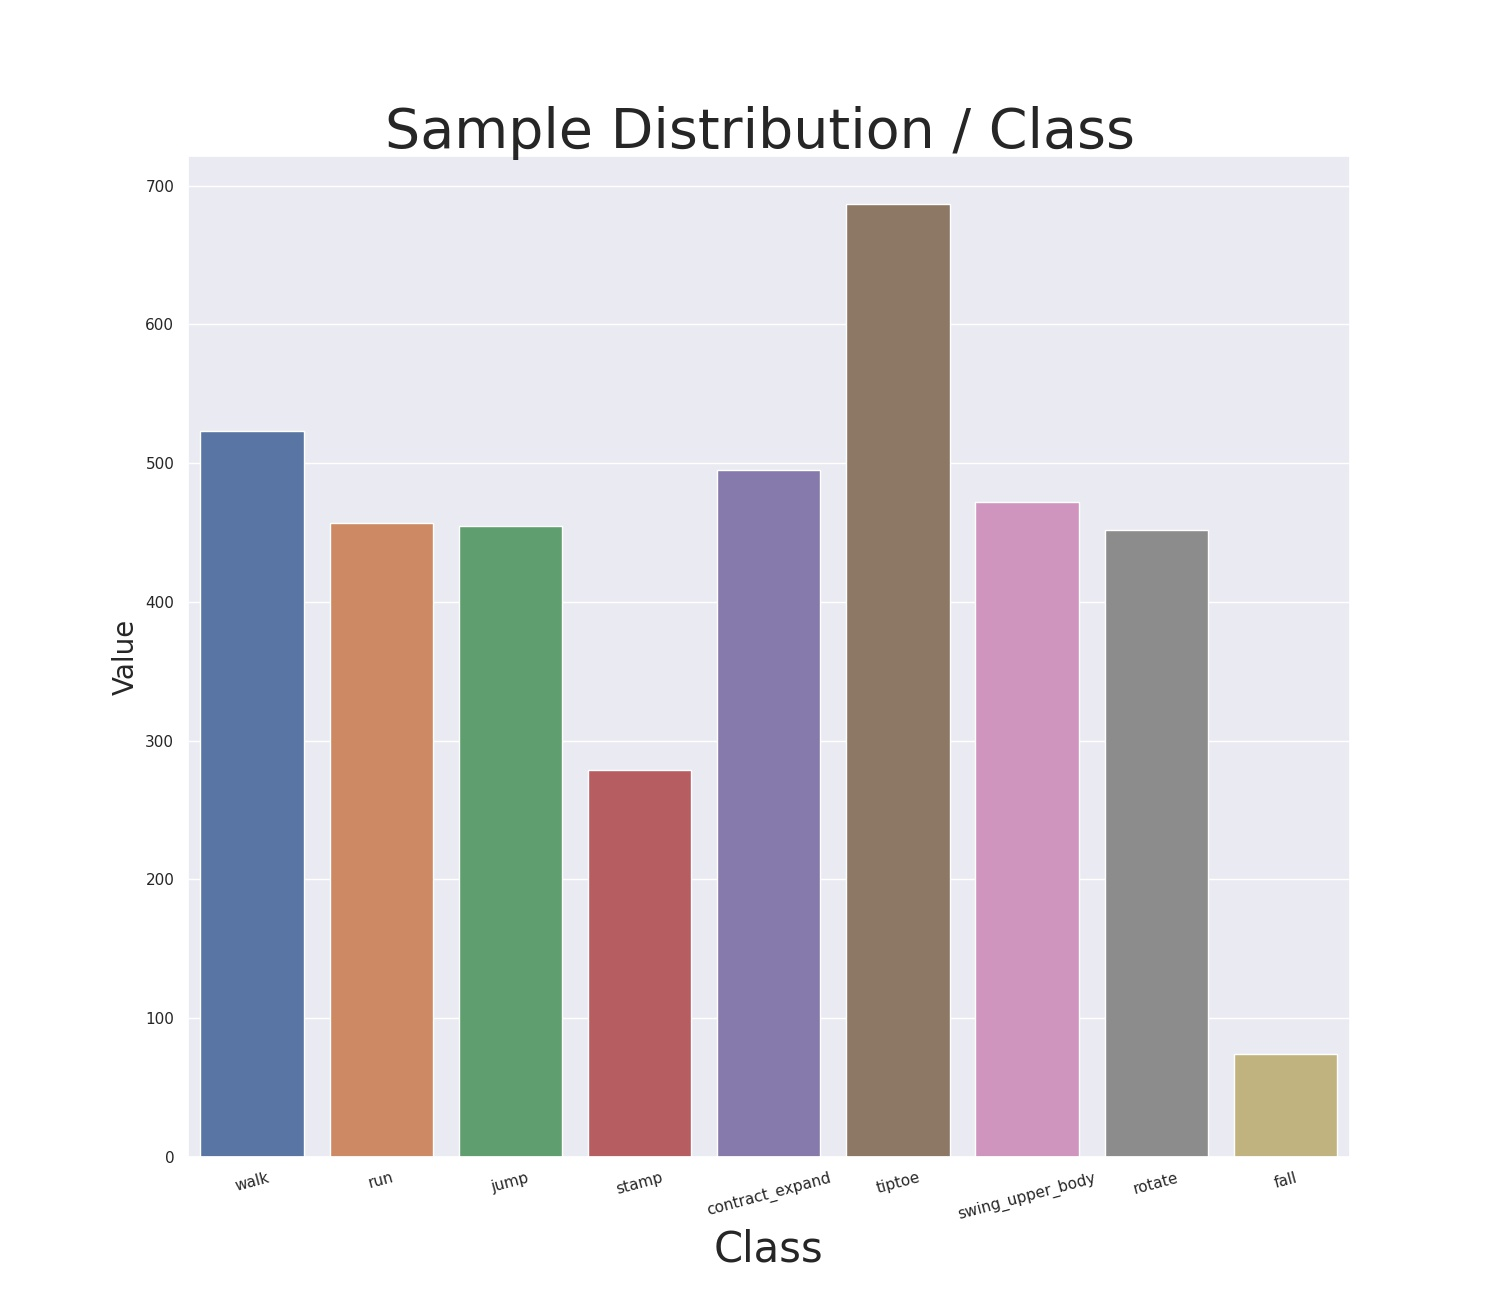
\includegraphics[height={320pt}, width={380pt}]{Thesis/images/bast_base_cls_dist.jpg}
\caption{Clips per each class for the \textit{bast-base} task}
\label{bast_base_cls_dist}
\end{figure}

\subsubsection{Bast-Eval}
\label{initial_analysis_bast_eval}
The \textit{bast-eval} dataset is imbalanced. Figure \ref{bast_eval_cls_dist} illustrates the variability in number of clips for the \textit{42} annotations. This variability is two-fold: first, globally in the number of clips across all the \textit{42} annotations, and second, locally within the nine tasks (base annotations) themselves as illustrated by the eight plots.

\begin{figure}[h]
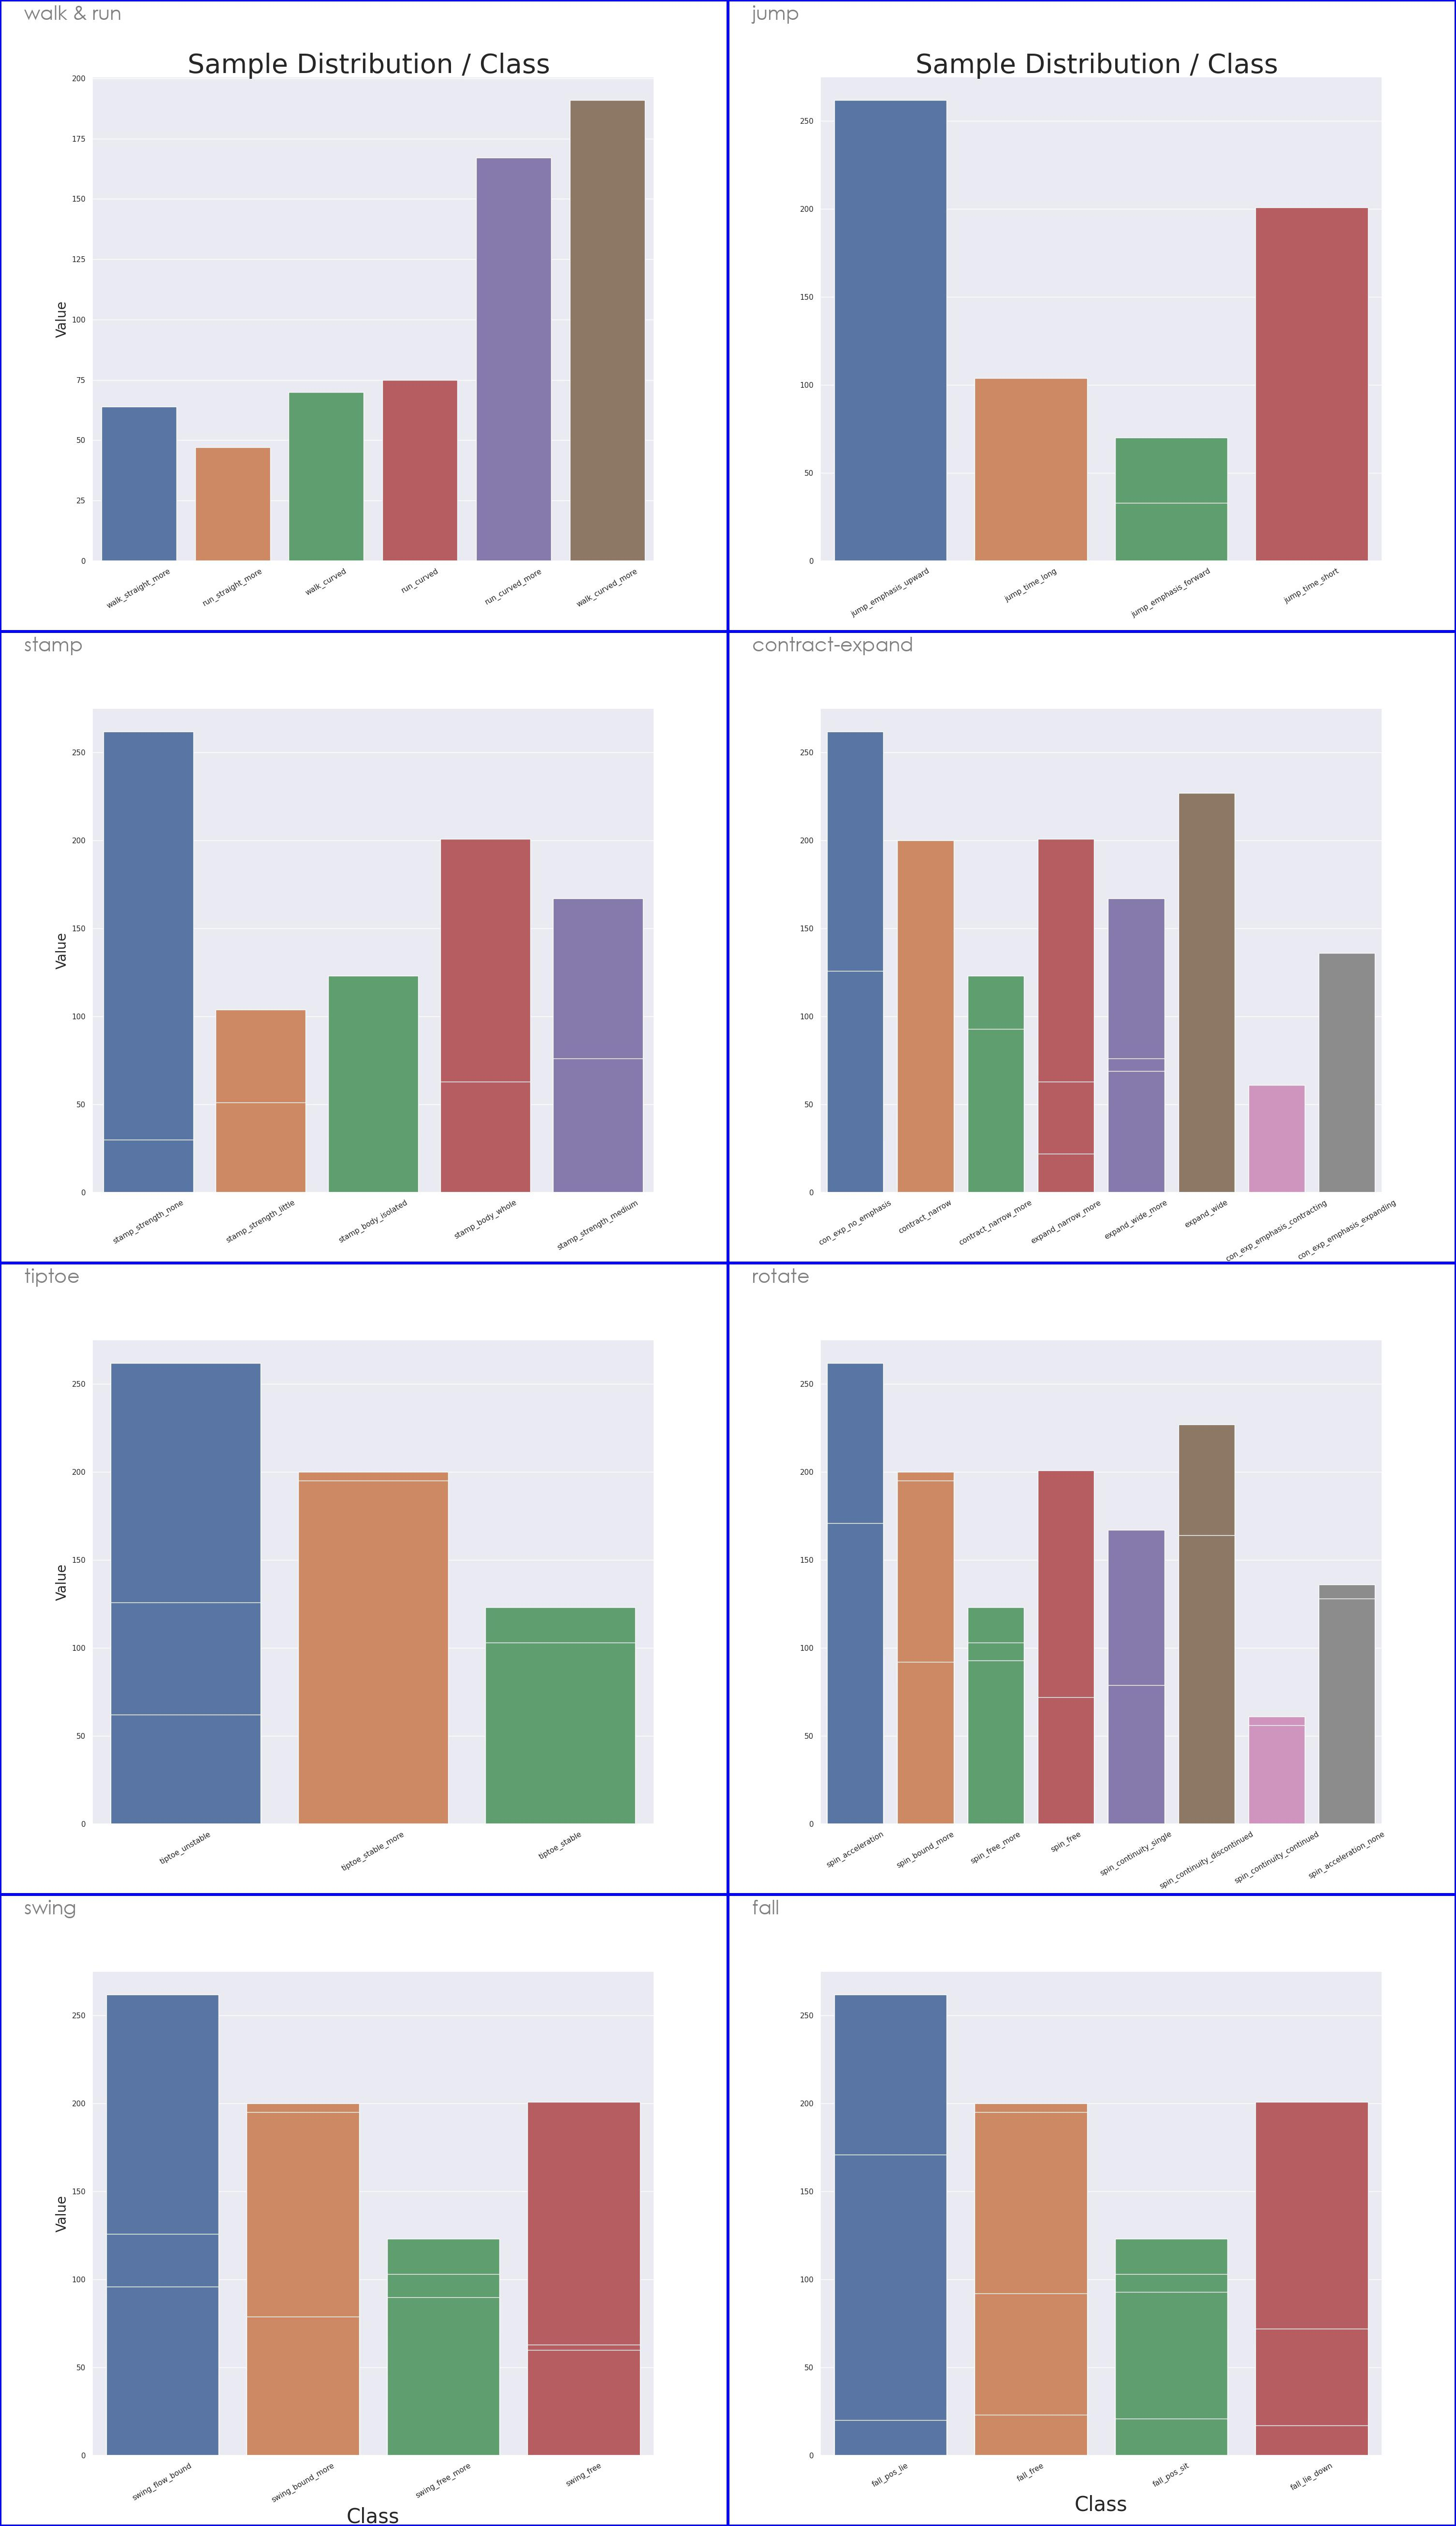
\includegraphics[height={650pt}, width={470pt}]{Thesis/images/bast_eval_cls_dist.jpg}
\caption{Clips per each class for the \textit{bast-eval} task}
\label{bast_eval_cls_dist}
\end{figure}

\noindent Globally, the number of clips per class varies from a minimum of $20$ for \textit{fall\_pose\_lie} to a maximum of $262$ for \textit{jump\_emphasis\_forward} with an average of 98 clips per class and a standard deviation of $61$. This shows severe imbalance. However, a deeper analysis reveals that this problem can be ameliorated to a certain extend. If we assume that at a certain part of the video, the model only has to deal with one task or at most two (e.g., \textit{tiptoe} and \textit{rotate}), then this means that only the variability of those particular tasks matters at any given time. In other words, we could narrow down the global variability to the local one, since at any given time, the person is performing one or a maximum of two of the nine tasks, and as a consequence, the model can narrow down the search space of the $42$ annotations. The reduction of the global variance of the dataset to the local one could be achieved by utilizing a pre-trained model on the \textit{bast-base} dataset. In this case, the pre-training of the model on the nine base categories could prime it better into drawing the distinction between the different evaluations.  Hence the hypothesis is: Will pre-training the model on the \textit{bast-base} dataset help solve the class imbalance problem of the \textit{bast-eval} dataset? Can we use transfer learn from the \textit{bast-base} task to further boost the performance of the model in the \textit{bast-eval} task? Section \ref{research_question_4} addresses these questions.

Locally, there is quite some variance for some of the tasks as well. For the \textit{walk} and \textit{run} task the \textit{curved\_more} evaluation has roughly double the amount of samples than the others. What matters, however, is not the variance in the number of samples among all evaluations of the same task but the variance among individual evaluations of the task. For example, for the \textit{jump} task, there are two evaluations, namely \textit{emphasis} and \textit{time-in-air}. Since we take into consideration the \textit{top-3} accuracy of the model, we are looking for three evaluations and not just one. This means that the variance in the values that \textit{emphasis} and \textit{time-in-air} individually take matters and not the variance in both of them taken together. Nevertheless, for this particular task the \textit{jump\_emphasis\_upward} and \textit{jump\_time\_short} still have more than double the number of samples than their counterparts. Below the results from the plots for the rest of the evaluations as listed:

\begin{itemize}
    \item \textit{stamp-strength}: \textit{none} and \textit{medium} have comparable numbers but \textit{little} has a much lower amount of samples.
    \item \textit{stamp-body-involvement}: \textit{body-whole} has double the annotations of \textit{body-isolated}.
    \item \textit{contract-expand-emphasis}: \textit{emphasis-contracting} is severely underrepresented 
    \item \textit{contract-expand-kinesphere}: no imbalance
    \item \textit{tiptoe}: slight imbalance
    \item \textit{spin-acceleration} and  \textit{spin-flow}: no imbalance
    \item \textit{spin-continuity}: \textit{continued} has little samples when compared to \textit{discontinued} and \textit{none}, which are roughly equal
    \item \textit{swing} and \textit{fall}: no imbalance
\end{itemize}

\noindent Overall, the dataset exhibits both global and local variance, and while the former can be mitigated and transformed to the latter, the problem of class imbalance remains on the local level. It remains an open problem, and while there are various over-sampling techniques using data augmentation strategies such as piecewise affine transformation, superpixel, gausian blurring, color inversion, and many more\footnote{\url{https://github.com/okankop/vidaug}}, that could be used on the under represented classes, they were not utilized in the scope of this thesis in the belief that the benefits would not have been able to override the fact that a better dataset was needed to begin with.

\subsection{Preliminary BAST Analysis}
\label{bast_initial_analysis}
\begin{table}[h!]
  \begin{center}
    \caption{Window-size and clip-length experiments for the \textit{bast-base} dataset using the I3D architecture}
    \label{tab:window_size_clip_length_i3d}
    \begin{tabular}{l|l|c|c|c}
      \textbf{clip-len} & \textbf{win-size} & \textbf{Top2 Acc (tr)} & \textbf{Top2 Acc (val)} & \textbf{Top2 Acc (test)}\\
      \hline
      10s & 5s & 85\% & 92.6\% & 96.3\% \\
      10s & None & 83\% & 93.5\% & 96.3\% \\
      6s & 3s & 89\% & 88\% & 91.4\% \\
      10s & 3s & 86.5\% & 88.6\% & 91.7\% \\
      8s & 4s & 83.4\% & 90.4\% & 91.7\% \\
    \end{tabular}
  \end{center}
\end{table}

\begin{table}[h!]
  \begin{center}
    \caption{Window-size and clip-length experiments for the \textit{bast-base} dataset using Omni-Sourced pre-training}
    \label{tab:window_size_clip_length_omni}
    \begin{tabular}{l|l|c|c|c}
      \textbf{clip-len} & \textbf{win-size} & \textbf{Top2 Acc (tr)} & \textbf{Top2 Acc (val)} & \textbf{Top2 Acc (test)}\\
      \hline
      10s & 5s & 85.3\% & 95.1\% & 97.31\% \\
      10s & None & 79.3\% & 92.7\% & 96.78\% \\
    \end{tabular}
  \end{center}
\end{table}

\noindent Finally, before the experiments proper, some experiments were run to determine the best size of the sliding window and clip length. The idea behind using a sliding window is to generate more clips given the relatively small dataset of 98 videos. Additionally, since each of the nine tasks is performed in a 30-second as a continuum, abruptly feeding portions of this segment might be detrimental the model's performance. The experiments listed at table \ref{tab:window_size_clip_length_i3d} were performed using the I3D architecture with a kinetics pre-training, while the experiments listed at table \ref{tab:window_size_clip_length_omni} were performed using SlowOnly with a Omni-Sourced dataset pre-training.

In conclusion, using a sliding window of 5-seconds with a clip length of 10-seconds gives us the benefit of a bigger dataset but also boosts the model's performance. While the benefits in performance are not so clear with the I3D architecture, it becomes clear with the Omni-Sourced pre-training where the window size boosts the validation accuracy by $2.4\%$ and the testing one by $0.53\%$.

\newpage
\section{Experiments}
\label{experiments}

In this section, experiments and results with respect to the five research questions laid down in Section \ref{research_objectives_and_research_questions}, that is, RQ1 (Section \ref{research_question_1}), RQ2 (Section \ref{research_question_2}), RQ3 (Section \ref{research_question_3}, RQ4 (Section \ref{research_question_4}), RQ5 (Section \ref{research_question_5}) are presented. We start off with the best classifier for the \textit{bast-base} task.

\subsection{Best Classifier for Base Annotations}
\label{research_question_1}

\fbox{\begin{minipage}{38.5em}
RQ1: Which is the best human action recognition (HAR) model for classifying the nine base movements (\textit{walk}, \textit{run}, \textit{jump}, \textit{stamp}, \textit{contract\expand}, \textit{tiptoe}, \textit{swing upper body}, \textit{rotate} and \textit{fall}) of the BAST analysis?
\end{minipage}}

\bigskip \bigskip
\noindent For the purpose of classifying the nine base annotations of the BAST analysis, 2D, as well as 3D ConvNets, were utilized. The models' architectures have been described in details at Sections \ref{2d_convolutional_models} and \ref{3d_convolutional_models} respectively. We start off with the 2D models below.

\subsubsection{2D Models}
Table \ref{tab:research_question_1_2d_models} shows the results for the 2D models. All the models that do not have a pre-training dataset specified under the 'Caveat' column have been pre-trained using the \textit{kinetics-400} dataset.

\bigskip
\noindent\textit{Note: `d` stands for dropout and `pr` stands for pre-training}

\begin{table}[h!]
  \begin{center}
    \caption{2D Models for the \textit{bast-base} task}
    \label{tab:research_question_1_2d_models}
    \begin{tabular}{l|l|c|c|c}
      \textbf{Model} & \textbf{Caveat} & \textbf{Top2 Acc (test)} & \textbf{Top2 Acc (val)} & \textbf{Mean Class Acc}\\
      \hline
      \multirow{2}{*}{TSM} & \textit{baseline} & 27.4\% & 87\% & \textbf{14.5\%}\\
       & \textit{0.65d} & 28.1\% & \textbf{88\%} & 13.5\%\\
      \hline
      \multirow{3}{*}{TSN} & \textit{baseline}  & 13.8\% & 34\% & 9.8\%\\
       & \textit{0.6d} & 24.1\% & 30\% & 7.8\%\\
       & \textit{diving-pr} & 18.3\% & 31.1\% & 9.0\%\\
      \hline
      \multirow{2}{*}{Tanet} & \textit{baseline} & \textbf{28.8\%} & 80\% & 13.0\%\\
       & \textit{0.7d} & 28.3\% & 82.5\% & \textbf{14.5\%}\\
      \hline
      \multirow{1}{*}{TIN} & \textit{baseline}& 19.7\% & 83.4\% & 9.6\%\\
      \hline
      \multirow{1}{*}{TRN} & \textit{baseline}& 25\% & 30\% & 25\%\\
      \hline
    \end{tabular}
  \end{center}
\end{table}

\noindent TSN, a relatively early work in ConvNet research for HAR, and TRN, both seem to be severely underfitting the task because these models' validation and testing accuracy are both very low. TSM, TIN, and Tanet, on the other hand, perform relatively well on the validation set (high validation accuracy) but fail to generalize for unseen samples (low testing accuracy). This means that they are overfitting the \textit{bast-base} task and serves to show its difficulty even though the nine actions of the \textit{bast-base} dataset are pretty straightforward. Of course, another reason for the overfit could be the relatively small BAST dataset at hand. Nevertheless, even increasing the dropout rate does not solve the overfitting problem for the 2D models. E.g., for Tanet, a $0.7$ dropout rate yielded only a $1\%$ in the \textit{top-2} validation accuracy and less than $1\%$ for the test accuracy. 

All of these 2D models avail certain tricks in their architecture in order to capture the temporal relations in a video, such as, for example, shifting the spatial channels. However, the fact that they fail to generalize for the \textit{bast-base} task shows that the 2D model family generally lacks the robust spatio-temporal reasoning capabilities offered by 3D models. This is the main reason behind their poor generalization capabilities. Another reason for it is the sparse sampling strategy that they use. The most common recommended strategy for these models, which was also used in this work, is a uniform sampling strategy of $1 \times 1 \times 8$. While it can be argued that such a sampling strategy might be enough for the base annotations of the \textit{bast-base} task, this almost certainly cannot be said for the fine-grained annotations of the \textit{bast-eval} task. 3D ConvNets, on the other hand, work with dense sampling strategies that typically sample many more frames than 2D models do and can extract more features from the data. Although, even 3D models sample just a fraction of the overall frames in the clip.

HAR models, in general, do not utilize all the frames of a video, given that this would tremendously increase the computational and time complexity of the model. Although there is some work on models that utilize all the frames \cite{liu2021no} in a refined manner, this thesis has exclusively focused on state-of-the-art models that use a sparse sampling strategy.

\bigskip
\noindent Figure \ref{fig:tsm_tanet_topk_accuracy} shows the \textit{top-k} accuracy for the Tanet and TSM models. Both have roughly the same performance and they both are performing very poorly for each class. Indeed, for the \textit{run}, \textit{tiptoe}, \textit{stamp}, \textit{contract/expand} and \textit{fall} tasks, the Tanet model has a negible, if not $0\%$ accuracy. A similar situation exists for TSM. Only when considering the \textit{top-3} accuracy we can say that the models are giving some rudimentary feedback on the performed action. The two tasks for which these models give any acceptable result are only \textit{jump} and \textit{swing-upper-body} and this only when considering the \textit{top-3} accuracy.

\noindent In conclusion, 2D HAR models are a poor choice for solving even the \textit{bast-base} dataset. As a consequence, they have not been tested at all for the \textit{bast-eval} dataset.

\begin{figure}[h]
\center
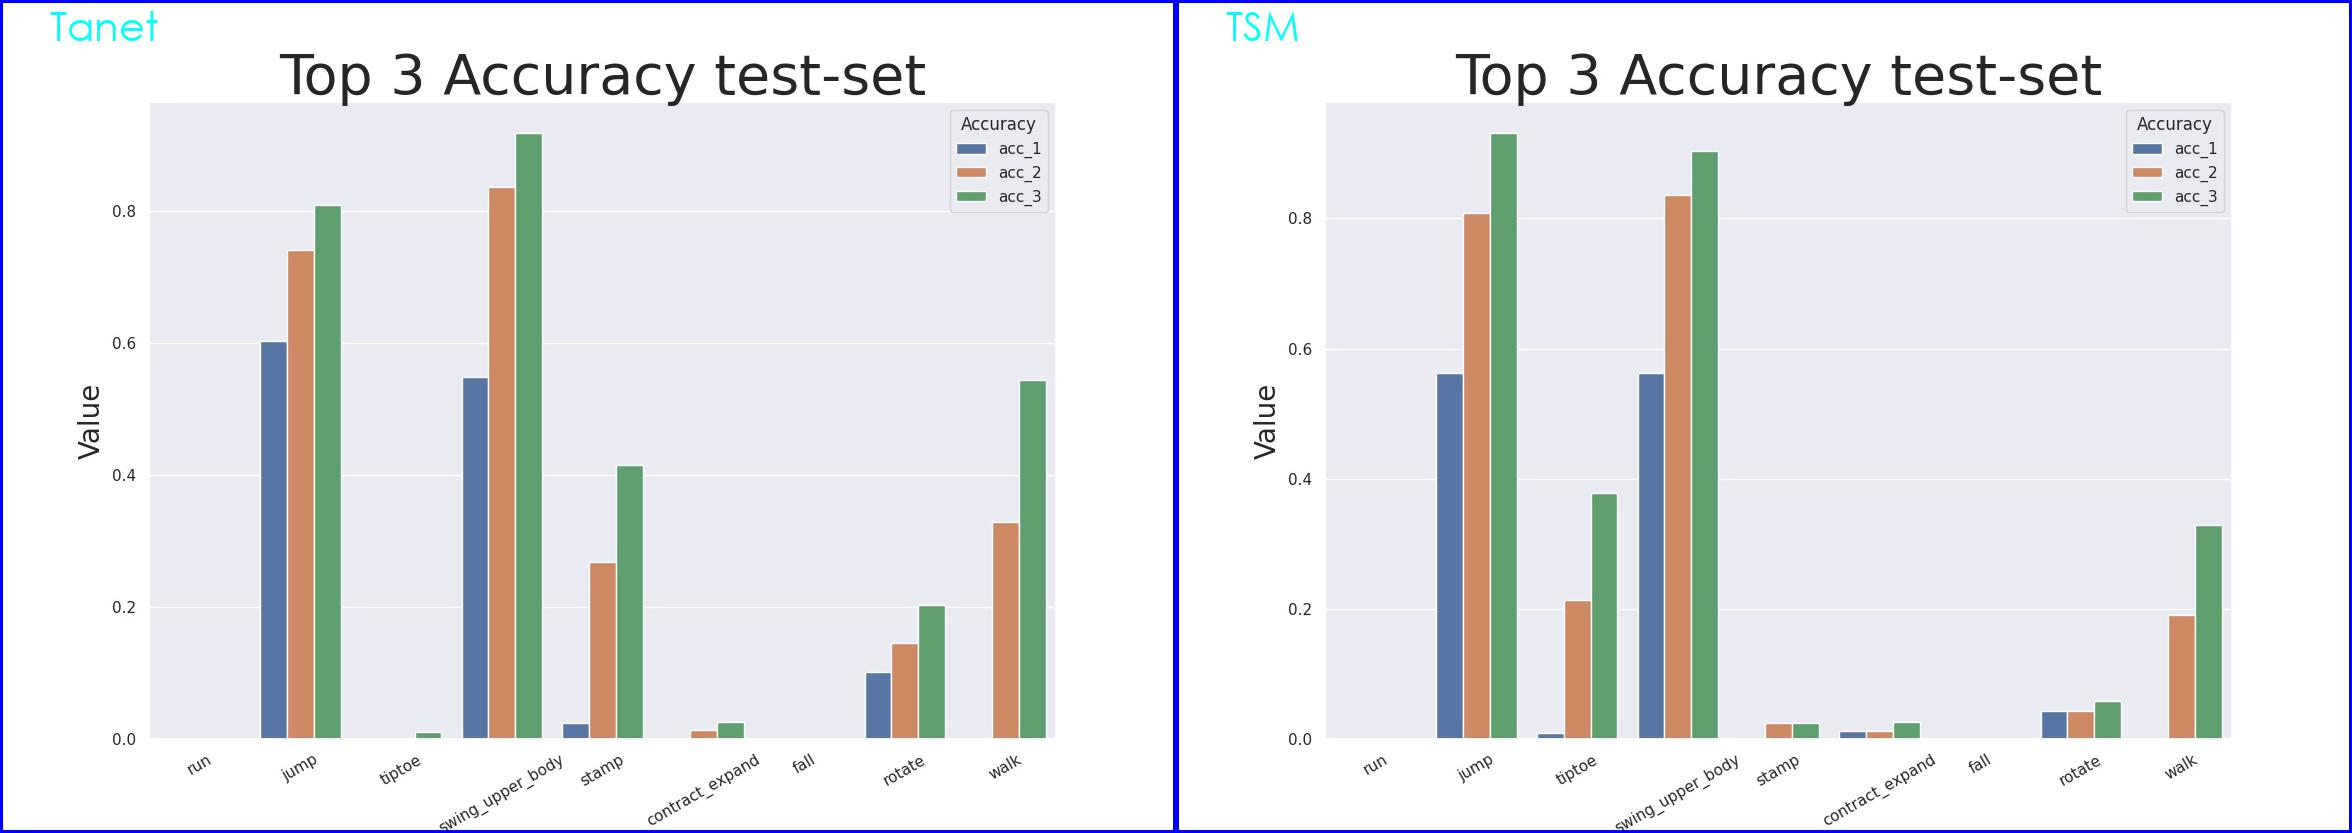
\includegraphics[height={150pt}, width={430pt}]{Thesis/images/tsm_tanet_acc_per_class.jpg}
\caption{Accuracy for each annotation of the \textit{bast-base} task for 2D models}
\label{fig:tsm_tanet_topk_accuracy}
\end{figure}


\subsubsection{3D Models}

Table \ref{tab:research_question_1_3d_models} shows the results of using 3D HAR models for the purposes of classifying the \textit{bast-base} dataset. A number of benchmark datasets were utilized for pre-training purposes including, among others, \textit{gym}, and \textit{ntu120} for PoseC3D-SlowOnly, \textit{omni-sourced} for SlowOnly and \textit{kinetics-400} for I3D and SlowFast.

\begin{table}[h!]
  \begin{center}
    \caption{3D Models for the \textit{bast-base} task}
    \label{tab:research_question_1_3d_models}
    \begin{tabular}{l|l|c|c|c|c}
      \textbf{Model} & \textbf{Caveat} & \textbf{Top1 Acc} & \textbf{Top2 Acc} & \textbf{Top2 Acc (val)} & \textbf{Mean Cls Acc}\\
      \hline
      \multirow{2}{*}{I3D} & \textit{baseline}& 87.2\% & 96.3\% & 92.6\% & 87.1\%\\
      & \textit{no dropout} & 20.9\% & 25.3\% & 86.4\% & 18.4\%\\
      \hline
      \multirow{1}{*}{SlowOnly} & \textit{omni-pr}& 92.1\% & \textbf{97.31\%} & 95.1\% & 91.7\%\\
      \hline
      \multirow{1}{*}{SlowFast} & \textit{baseline}& 90.6\% & 96\% & 95\% & 90\%\\
      \hline
      \multirow{1}{*}{CSN} & \textit{baseline} & - & - & 30\% & -\\
      \hline
      \multirow{7}{*}{PoseC3D} & \textit{gym-pr}& 88.9\% & 95.4\% & 94\% & 88.6\%\\
      & \textit{gym-0.7d}& 90.61\% & 95.5\% & 97.1\% & 90\%\\
      & \textit{ntu60-pr}& 89.25\% & 95.5\% & 96.3\% & 89.2\%\\
      & \textit{ntu120-0.8d}& 91.5\%& 96.25\% & \textcolor{blue}{\textbf{97.8\%}} & 91.1\%\\
      & \textit{ntu120-0.8d-54x1x1}& 87.0\% & 93.9\% & 96.9\% & 85.7\%\\
      & \textit{ntu120-0.8d-64x1x1}& 88.9\% & 96.1\% & 97.6\% & 91\%\\
      & \textit{kinetics-ucf}& \textcolor{blue}{\textbf{92.32\%}} & \textcolor{blue}{\textbf{97.27\%}} & 97.7\% & \textcolor{blue}{\textbf{92.52\%}}\\
      & \textit{kinetics-0.7d-32x1x1}& 90.44\% & 96.93\% & 97.4\% & 89.6\%\\
    \end{tabular}
  \end{center}
\end{table}

\noindent For the evaluation of the 3D models we consider four metrics in total, namely \textit{top-1} and \textit{top-2} testing accuracy, \textit{top-2} validation accuracy, and finally the \textit{mean class accuracy} for the testing set. From the table, we can see that PoseC3D-SlowOnly is the best model, as it achieves excellent results on all of these metrics. It is followed closely by SlowOnly with an \textit{omni-sourced} pre-training, which also serves to show the benefits of using such pre-training weights. Both of these models surpassed a $97\%$ \textit{top-2} test accuracy, while PoseC3D also achieved a \textit{92.52\%} \textit{mean class accuracy}. This shows that the model generalizes very well even for the \textit{top-1} accuracy. Moreover, given the good performances of I3D and SlowFast, we may conclude that 3D HAR models achieve an excellent job at classifying the \textit{bast-base} dataset. The only exception was CSN, which could not properly learn the task and had a disastrous performance of $30\%$ accuracy in the validation set.

\bigskip
\noindent For the I3D model, a dense sampling strategy of $32 \times 1 \times 1$ was used. \textit{Omni-Sourced} SlowOnly used a $8 \times 8 \times 1$ dense sampling strategy, while SlowFast used a $32 \times 2 \times 1$. Finally, the preferred strategy for PoseC3D was a dense sampling of $48 \times 1 \times 1$. Unless specified, all experiments with these models use these types of dense sampling strategies through this thesis. For PoseC3D, three experiments were also run with different sampling strategies, namely one with a dense sampling strategy of $54 \times 1 \times 1$, another with $64 \times 1 \times 1$, and finally with $32 \times 1 \times 1$. Although the models with these sampling strategies achieved good results, with the latter achieving a $96.93\%$ \textit{top-2} accuracy, they were not able to surpass the performance of the baseline sampling strategy.

\bigskip
\noindent Figure \ref{fig:3d_models_base_loss} compares the training loss for the PoseC3D and SlowOnly models. The latter has a clear advantage taking the loss to almost 0, in contrast to SlowOnly, which could not lower it more than $0.5$. Since PoseC3D was able to lower the loss so much, it is conceivable that it could even achieve a perfect $100\%$ accuracy on a bigger dataset. On the other hand, since SlowOnly seems not to have exhausted its capabilities (given the trend of the curve), it is also possible that it would achieve better results with a more robust dataset. 

\begin{figure}[h]
\center
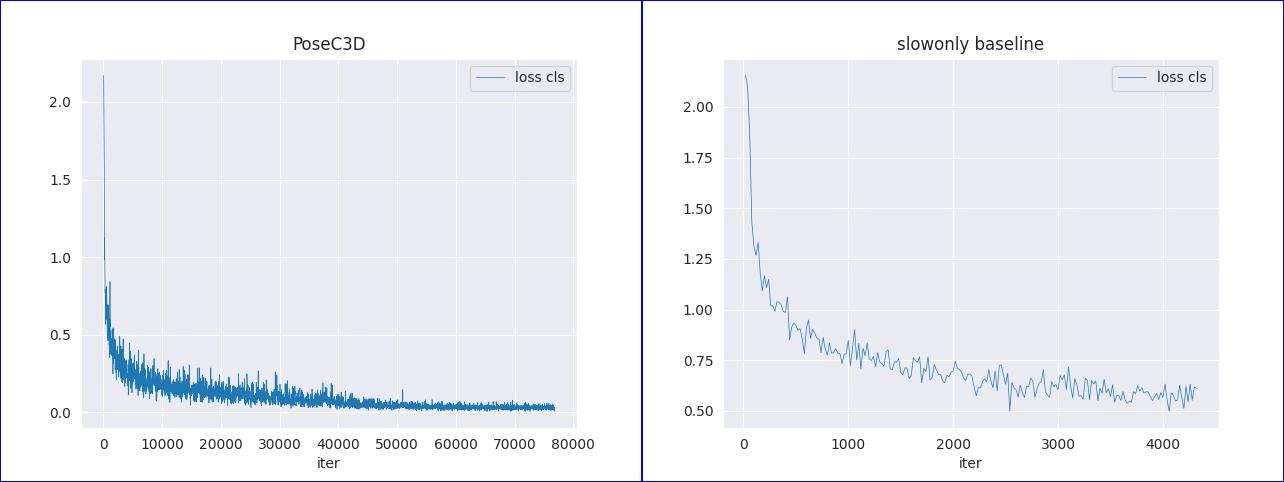
\includegraphics[height={150pt}, width={430pt}]{Thesis/images/3D_models_base_loss.jpg}
\caption{Training loss for PoseC3D and SlowOnly}
\label{fig:3d_models_base_loss}
\end{figure}

\bigskip
\noindent Figure \ref{fig:3d_models_top_class_accuracy} shows the \textit{top-k} accuracy for each class for the four top performing 3D models, namely I3D, SlowFast, SlowOnly, and PoseC3D. In general all models achieve pretty good results with the \textit{top-1} accuracy, which are only reinforced when considering the \textit{top-2} accuracy. The top model, PoseC3D is able to perfectly recognize the \textit{walk}, \textit{fall}, and \textit{run} actions. Moreover, when considering the \textit{top-2} accuracy, then it is able to also perfectly classify \textit{jump}, and \textit{tiptoe}. The classification of the four remaining actions is also quite satisfactory by this model. Indeed, PoseC3D is the model that yields the best results for the \textit{bast-base} task.

\bigskip
\noindent The least performing model is I3D, which has an inferior architecture when compared to the other models, given that it came out in 2017 (in contrast PoseC3D came out in 2021). However, when considering the \textit{top-2} accuracy, its performance significantly improves. Indeed I3D shows the biggest performance improvement when considering a \textit{top-2} accuracy, namely of $9.1\%$. The SlowOnly architecture based on an \textit{omni-sourced} training is performing better than the SlowFast architecture, which includes both the Slow and the Fast stream, and which is based on an \textit{kinetics-400} pre-training. This demonstrates the immense importance of transfer learning in HAR tasks, especially when the target dataset is small. Indeed, the architecture of SlowFast is supposed to be superior to SlowOnly because it includes both streams. However, a pre-training on \textit{omni-source} makes the SlowOnly model fare better than its counterpart. Transfer learning for the tasks at hand is examined in great details in Section \ref{research_question_4}.

\bigskip
\noindent Taking a bird's eye view among the performance of all the four models, the hardest actions to learn, when considering a \textit{top-1} accuracy, are \textit{stamp}, \textit{contract-expand}, and \textit{swing-upper-body}. However, when considering the \textit{top-2} accuracy, we can conclude that the models are also learning these three tasks very well. Moreover, it is very likely that these 3D models would also be perfectly able to capture these actions if we had a bigger dataset at our disposal, as explained above through the loss plots. One happy observation is that all models recognize the \textit{fall} action with a very high accuracy even though this was the action for which we had the least amount of samples for. In contrast, 2D models, for example, were unable to get even one classification right for the \textit{fall} task. This again shows the potency of the 3D ConvNet models for human action recognition.

\begin{figure}[h]
\center
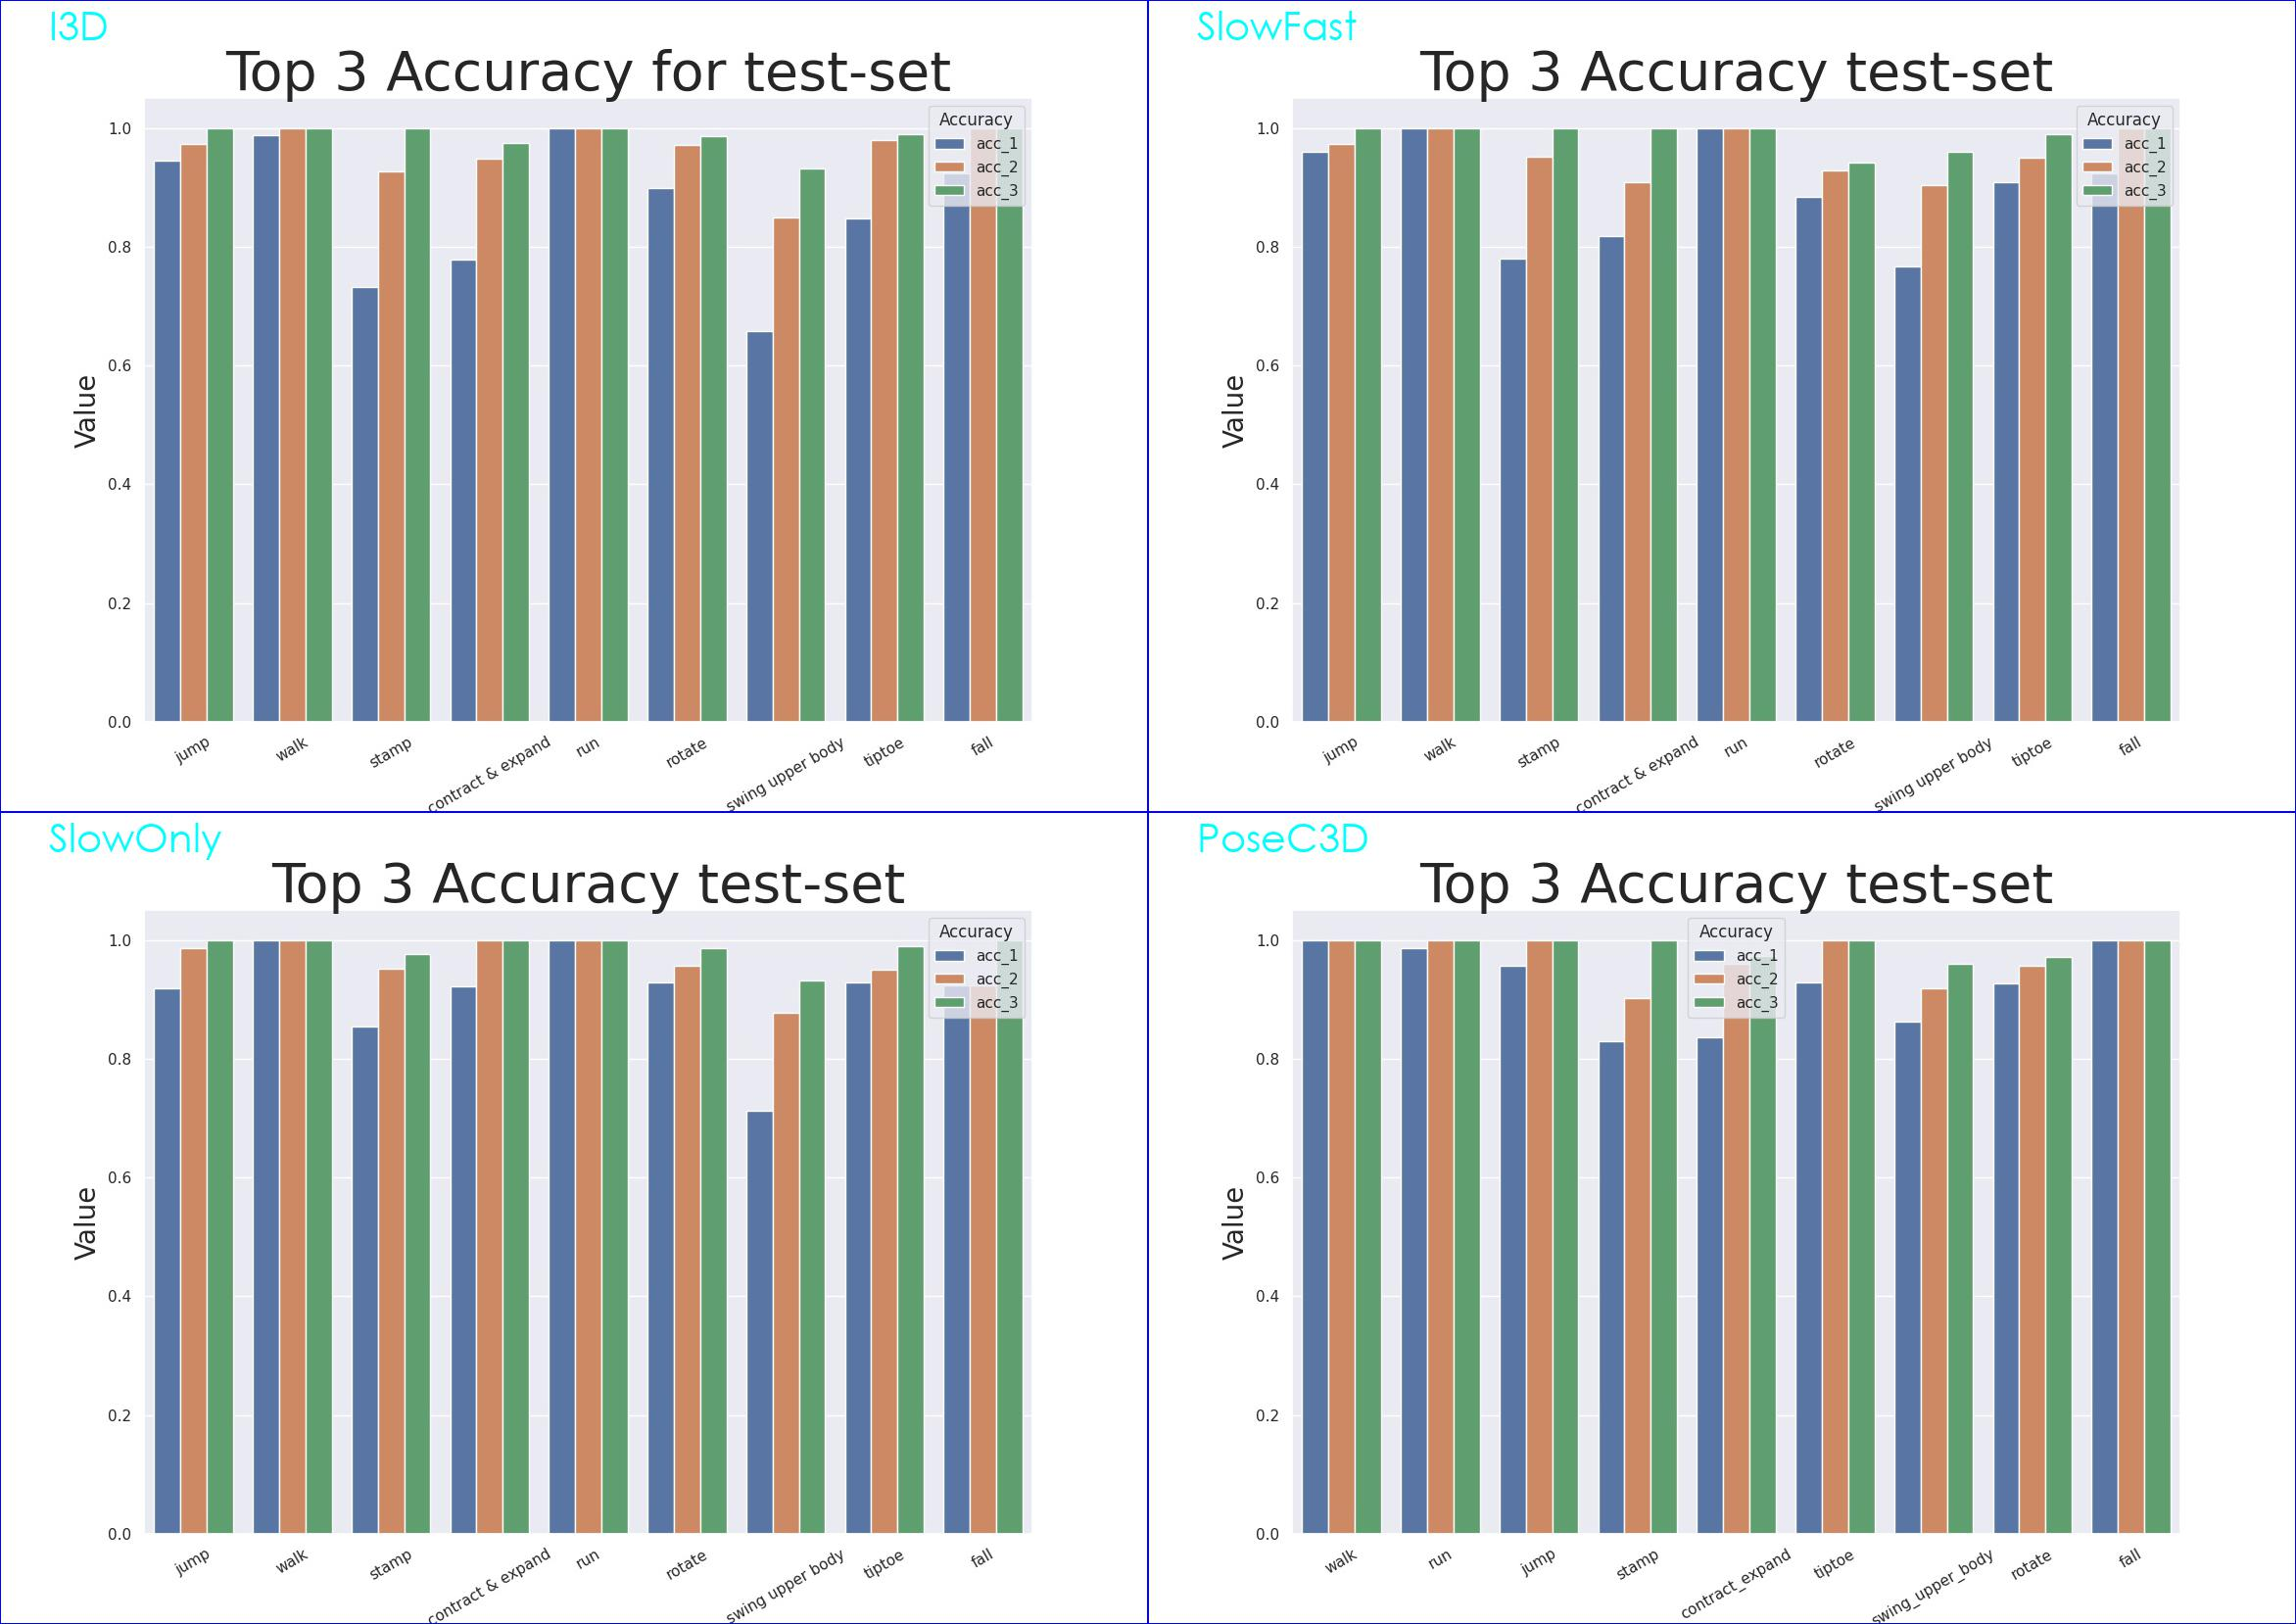
\includegraphics[height={330pt}, width={440pt}]{Thesis/images/3D_acc_per_class.jpg}
\caption{Accuracy for each annotation of the \textit{bast-base} task for 3D models}
\label{fig:3d_models_top_class_accuracy}
\end{figure}

\bigskip
\noindent\textbf{Training speed}: At table \ref{tab:research_question_1_training_speed}, we compare the training speed of the different 2D and 3D architectures that were presented above. The time is shown in seconds and consists of the iterations within an epoch. The training speed does not have much consequence when using powerful GPUs to train such models, but it can be important for not-so-powerful machines. For the purpose of this work 4 GPUs were used, namely two \textit{Geforce RTX 3090} 24GB each and two \textit{Geforce RTX 2080 Ti} 11GB each. The latter were connected via NVLink and made available through Cuda P2P\footnote{\url{https://medium.com/gpgpu/multi-gpu-programming-6768eeb42e2c}}; hence it was possible to harness them together.

\begin{table}[h!]
  \begin{center}
    \caption{Training speed of all models}
    \label{tab:research_question_1_training_speed}
    \begin{tabular}{l|c|c|c|c}
      \textbf{Model} & \textbf{Fastest epoch} & \textbf{Slowest epoch} & \textbf{Average iter time} & \textbf{Time std over epochs}\\
      \hline
      I3D & 3.3 & 8.3 & 4.5 & 0.9\\
      SlowOnly & 2.0 & 2.9 & 2.4 & 0.14 \\
      SlowFast & 3.9 & 14.6 & 9.1 & 2.0\\
      \textbf{PoseC3D} & 0.7 & 10.4 & 2.1 & 0.8\\
      TSM & 0.7 & 0.8 & 0.77 & 0.07\\
      \textbf{TSN} & 0.37 & 0.39 & 0.38 & 0.049\\
      Tanet & 0.48 & 0.52 & 0.51 & 0.056\\
      TIN & 0.41 & 0.43 & 0.42 & 0.0031\\
      TRN & 0.49 & 0.66 & 0.53 & 0.012\\
    \end{tabular}
  \end{center}
\end{table}

\noindent As is to be expected, we can see a significant gap in the training speed between the lighter 2D and heavier 3D models, with the latter being at least 2.7 times as fast as the former. The happy exception is the PoseC3D model, which is relatively fast compared to other 3D models and even comparable to the speed of 2D models. This is an advantageous trait of PoseC3D and is possible because it works on pose data. The other models that work on the RGB and optical flow modalities need to decode and pre-process images, which is computationally expensive and hence increases the training time.

\bigskip \bigskip
\noindent \textbf{Model complexity}: Finally, Table \ref{tab:research_question_1_complexity} below compares the complexity of the different architectures that were presented above. Specifically, it presents the number of parameters (in millions) and the number of flops (in giga). Both have been approximated and may not be completely accurate.

\begin{table}[h!]
  \begin{center}
    \caption{Model complexity}
    \label{tab:research_question_1_complexity}
    \begin{tabular}{l|c|c|c|c}
      \textbf{Model} & \textbf{Params (M)} & \textbf{Flops (G)}\\
      \hline
      I3D & 27.24 & 43.56\\
      SlowOnly & 31.65 & 54.86\\
      SlowFast & 34.48 & 36.44\\
      \textbf{PoseC3D} & 2.02 & 15.9\\
      TSM & 23.53 & 43.05\\
      TSN & 23.61 & 16.14\\
      Tanet & 24.79 & 43.06\\
      TIN & 23.56 & 43.05\\
      TRN & 26.34 & 43.06\\
    \end{tabular}
  \end{center}
\end{table}

\bigskip
\noindent Again, 2D models are generally lighter than the 3D ones. The main reason for this is that they use 2D instead of 3D convolutions, and the latter have more parameters to train than the former. The one exception remains PoseC3D, which has an excellent complexity, namely only 2M parameters, and only 15.9GFLOPs. Compared to other 3D models, it has as much as $14$ times less parameters and $3$ times less flops. What is more, this complexity is even superior to the complexity of the 2D models. This splendid complexity is another major point in favor of PoseC3D as it can be beneficial for deploying in production settings.

\bigskip \bigskip
\noindent \textbf{Conclusion:} Taking into consideration the model's performance, its \textit{top-1}, \textit{top-2} accuracy as well as the \textit{mean class accuracy}, we concluded that PoseC3D is the best model for our task. This architecture, moreover is extremely lightweight and very fast to train, only adding to its benefits.


\newpage
\subsection{Best Classifer for Evaluation Annotations}
\label{research_question_2}

\fbox{\begin{minipage}{38.5em}
RQ2: Which is the best human action recognition (HAR) model for classifying the 42 fine-grained annotations of the nine BAST task's evaluations? Would it be possible to automatize the BAST evaluation process so that certified trainers are no longer needed?
\end{minipage}}

\bigskip
\noindent In the previous chapter, we saw that 3D ConvNets achieved an excellent performance in the \textit{bast-base} task. Specifically, the best model, PoseC3D, had a very high accuracy and was very lightweight, thus making it a natural choice for production. In contrast, 2D models were either overfitting or underfitting the task altogether. Hence, for the \textit{bast-eval} task, we only explore 3D HAR models and entirely disregard the 2D ones. As already discussed in Section \ref{initial_analysis} the \textit{bast-eval} task is a challenging task due to the difficulty that the $42$ fine-grained actions (see Section \ref{background_bast} for details) present, as well as the severe data insufficiency and imbalance problem that the BAST dataset under disposal has. With this in mind, below we present the results.

Table \ref{tab:research_question_2_3d_models} below shows the result for fine-tuning 3D HAR models on the \textit{bast-eval} task. I3D used a \textit{kinetics} pre-training, SlowOnly used an \textit{omni-sourced} pre-training. Finally, PoseC3D used a variety of different datasets for pre-training, such as the \textit{gym} dataset or the \textit{bast-base} itself.

\bigskip
\noindent\textit{Note: `d` stands for dropout, `pr` stands for pre-training, and `bb` stands for bast-base.}

\bigskip
\begin{table}[h!]
  \begin{center}
    \caption{3D Models for the \textit{bast-eval} task}
    \label{tab:research_question_2_3d_models}
    \begin{tabular}{l|l|c|c|c}
      \textbf{Model} & \textbf{Caveat} & \textbf{Top3 Acc (test)} & \textbf{Top3 Acc (val)} & \textbf{Mean Class Acc}\\
      \hline
      \multirow{5}{*}{I3D} & \textit{-} & 59.5\% & 54.7\% & 25.4\%\\
      & \textit{0.4d}& 27\% & 63\% & 5.4\%\\
      & \textit{0.65d}& 22\% & 58\% & 9.8\%\\
      & \textit{0.6d-48x3x1}& 66\% & 59\% & 21\%\\
      \hline
      \multirow{2}{*}{SlowOnly} & \textit{bb-pr-8x8x1} & 60.3\% & 64.4\% & 24.6\%\\
      & \textit{bb-pr-0.6d-16x8x1} & 71\% & 67.6\% & 25.64\%\\
      \hline
      \multirow{4}{*}{PoseC3D} & \textit{gym-pr} & 69\% & 69.4\% & 22\%\\
      & \textit{gym-bb-pr-0.65d}& 72.2\% & 72.3\% & 32.5\%\\
      & \textit{ntu120-pr-0.7d}& 71.2\% & \textcolor{blue}{\textbf{74.9\%}} & 32.2\%\\
      & \textit{ntu120-pr-0.8d}& 75.7\% & 68.5\% & 23.6\%\\
      & \textit{bb-pr-64x1x1-0.6d}& \textcolor{blue}{\textbf{77.39\%}} & 72.68\% & \textcolor{blue}{\textbf{33.19\%}}\\
    \end{tabular}
  \end{center}
\end{table}

The 3D models used for this task are I3D, SlowOnly, and PoseC3D. The primary considered evaluation metric for the \textit{bast-eval} task, as elaborated in Section \ref{model_evaluation}, is the \textit{top-3} test accuracy. We can also take a bit into account the \textit{mean class accuracy} but only with caution since it is calculated for the \textit{top-1} accuracy. Results show that PoseC3D has a clear superior performance when compared to both I3D and SlowOnly. With a \textit{bast-base} pre-training, it was able to achieve a $77.39\%$ \textit{top-3} accuracy, which is very good considering the difficulties of the task at hand. The experiments of PoseC3D were usually run with the conventional $48 \times 1 \times 1$ sampling strategy. However, the top performance was rather achieved with an even denser sampling strategy, namely a $64 \times 1 \times 1$ sampling strategy. This makes sense because the actions of the \textit{bast-eval} task are fine-grained, and more information is needed in order to capture them correctly. In general, we observe that I3D and SlowOnly also achieve their top performances by particularly denser sampling strategies. For the coarse actions of the \textit{bast-base} task, on the other hand, a sparser dense strategy did the job, and in the case of PoseC3D, resulted in models that overfit the \textit{bast-base} task.

It is also conspicuous that a pre-training with the \textit{bast-base} dataset is very helpful for the \textit{bast-eval} dataset. These results are further discussed in Section \ref{research_question_4_3} and \ref{research_question_4_4}. The other two models, I3D, and SlowOnly also perform relatively well considering the toughness of the task. SlowOnly achieved as much as a $71\%$ testing accuracy with an $16 \times 8 \times 1$ dense sampling strategy, while I3D achieved $66\%$ using a $48 \times 3 \times 1$ dense sampling strategy. Therefore the conclusion is that the sampling strategy is a critical hyper-parameter choice because if we use the conventional sampling strategies that were used for the \textit{bast-base} task, the models have a much lower accuracy as they need more frames to correctly capture the fine-grained actions of the \textit{bast-eval} task.

\bigskip
\noindent Both I3D and SlowOnly (with an $8 \times 8 \times 1$ sampling strategy) converge to the best epoch quite early, e.g., in the case of SlowOnly, it converged in 27 epochs, while \textit{I3D-0.6d-48x3x1} converged in just $15$ epochs. \textit{PoseC3D} models on the other hand take many epochs to converge, namely in the case of \textit{PoseC3D-ntu120-pr-0.8d} (which used the conventional $42 \times 1 \times 1$ sampling strategy), it took $225$ epochs to converge. First, this serves to demonstrate again that the dataset under disposal is not enough for the \textit{bast-eval} task because the models are not able to keep learning but rather converge fairly quickly. Second, it also shows the complexity of the \textit{bast-eval} task. However, the fact that PoseC3D models were able to keep learning even under these conditions proves the superiority of skeleton models compared to conventional models that exploit RGB frames or optical flow. On the other hand, the SlowOnly model that used an $16 \times 8 \times 1$ sampling strategy also kept learning and only converged at epoch $95$. This again supports the finding that the sampling strategy is also crucial for learning fine-grained actions such as the actions of the \textit{bast-eval} task are.

\bigskip
\noindent Figure \ref{fig:3d_models_eval_loss} shows the loss for the three models. They all have similar losses. However, for the SlowOnly ($8 \times 8 \times 1$ sampling strategy) and I3D models, it looks like the loss could have been further reduced as it had not yet degraded into a linear function. However, because the models converged quite early on, this was not the case. Hence, it seems very likely that both of these models would have continued to learn and improve with a proper dataset. PoseC3D, on the other hand, seems to have exhausted its capabilities as the hyperbole slowly degenerated into a linear function. Nevertheless, a bigger and more robust dataset could have also been instrumental in PoseC3D achieving better results. Indeed, in the previous section, we saw that the loss for the \textit{bast-base} task was almost reduced to zero by this particular model.

\begin{figure}[h]
\center
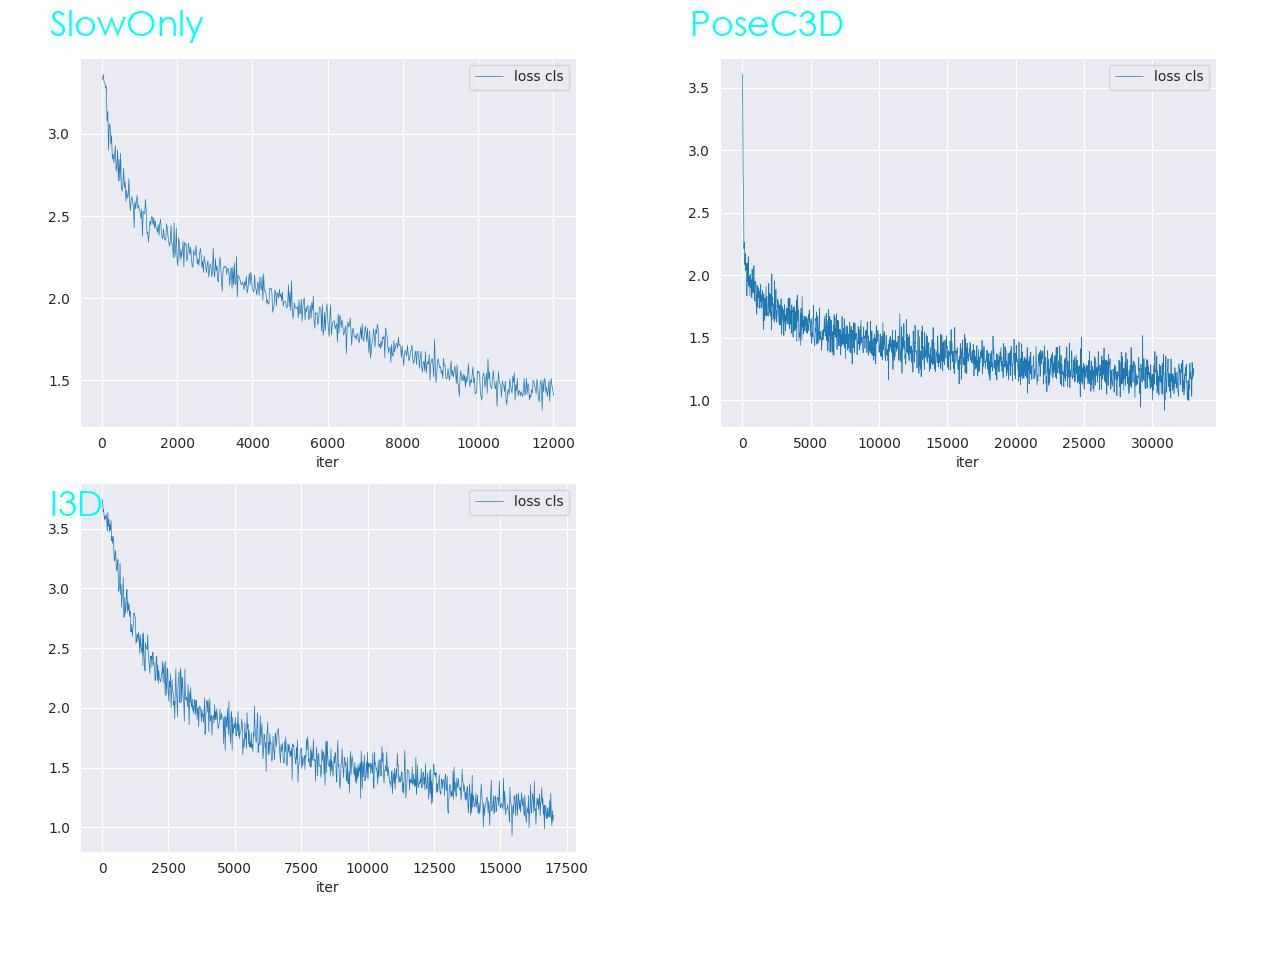
\includegraphics[height={300pt}, width={430pt}]{Thesis/images/3D_models_eval_loss.jpg}
\caption{Training loss for PoseC3D, SlowOnly, and I3D on the \textit{bast-eval} task}
\label{fig:3d_models_eval_loss}
\end{figure}

\begin{figure}[h]
\center
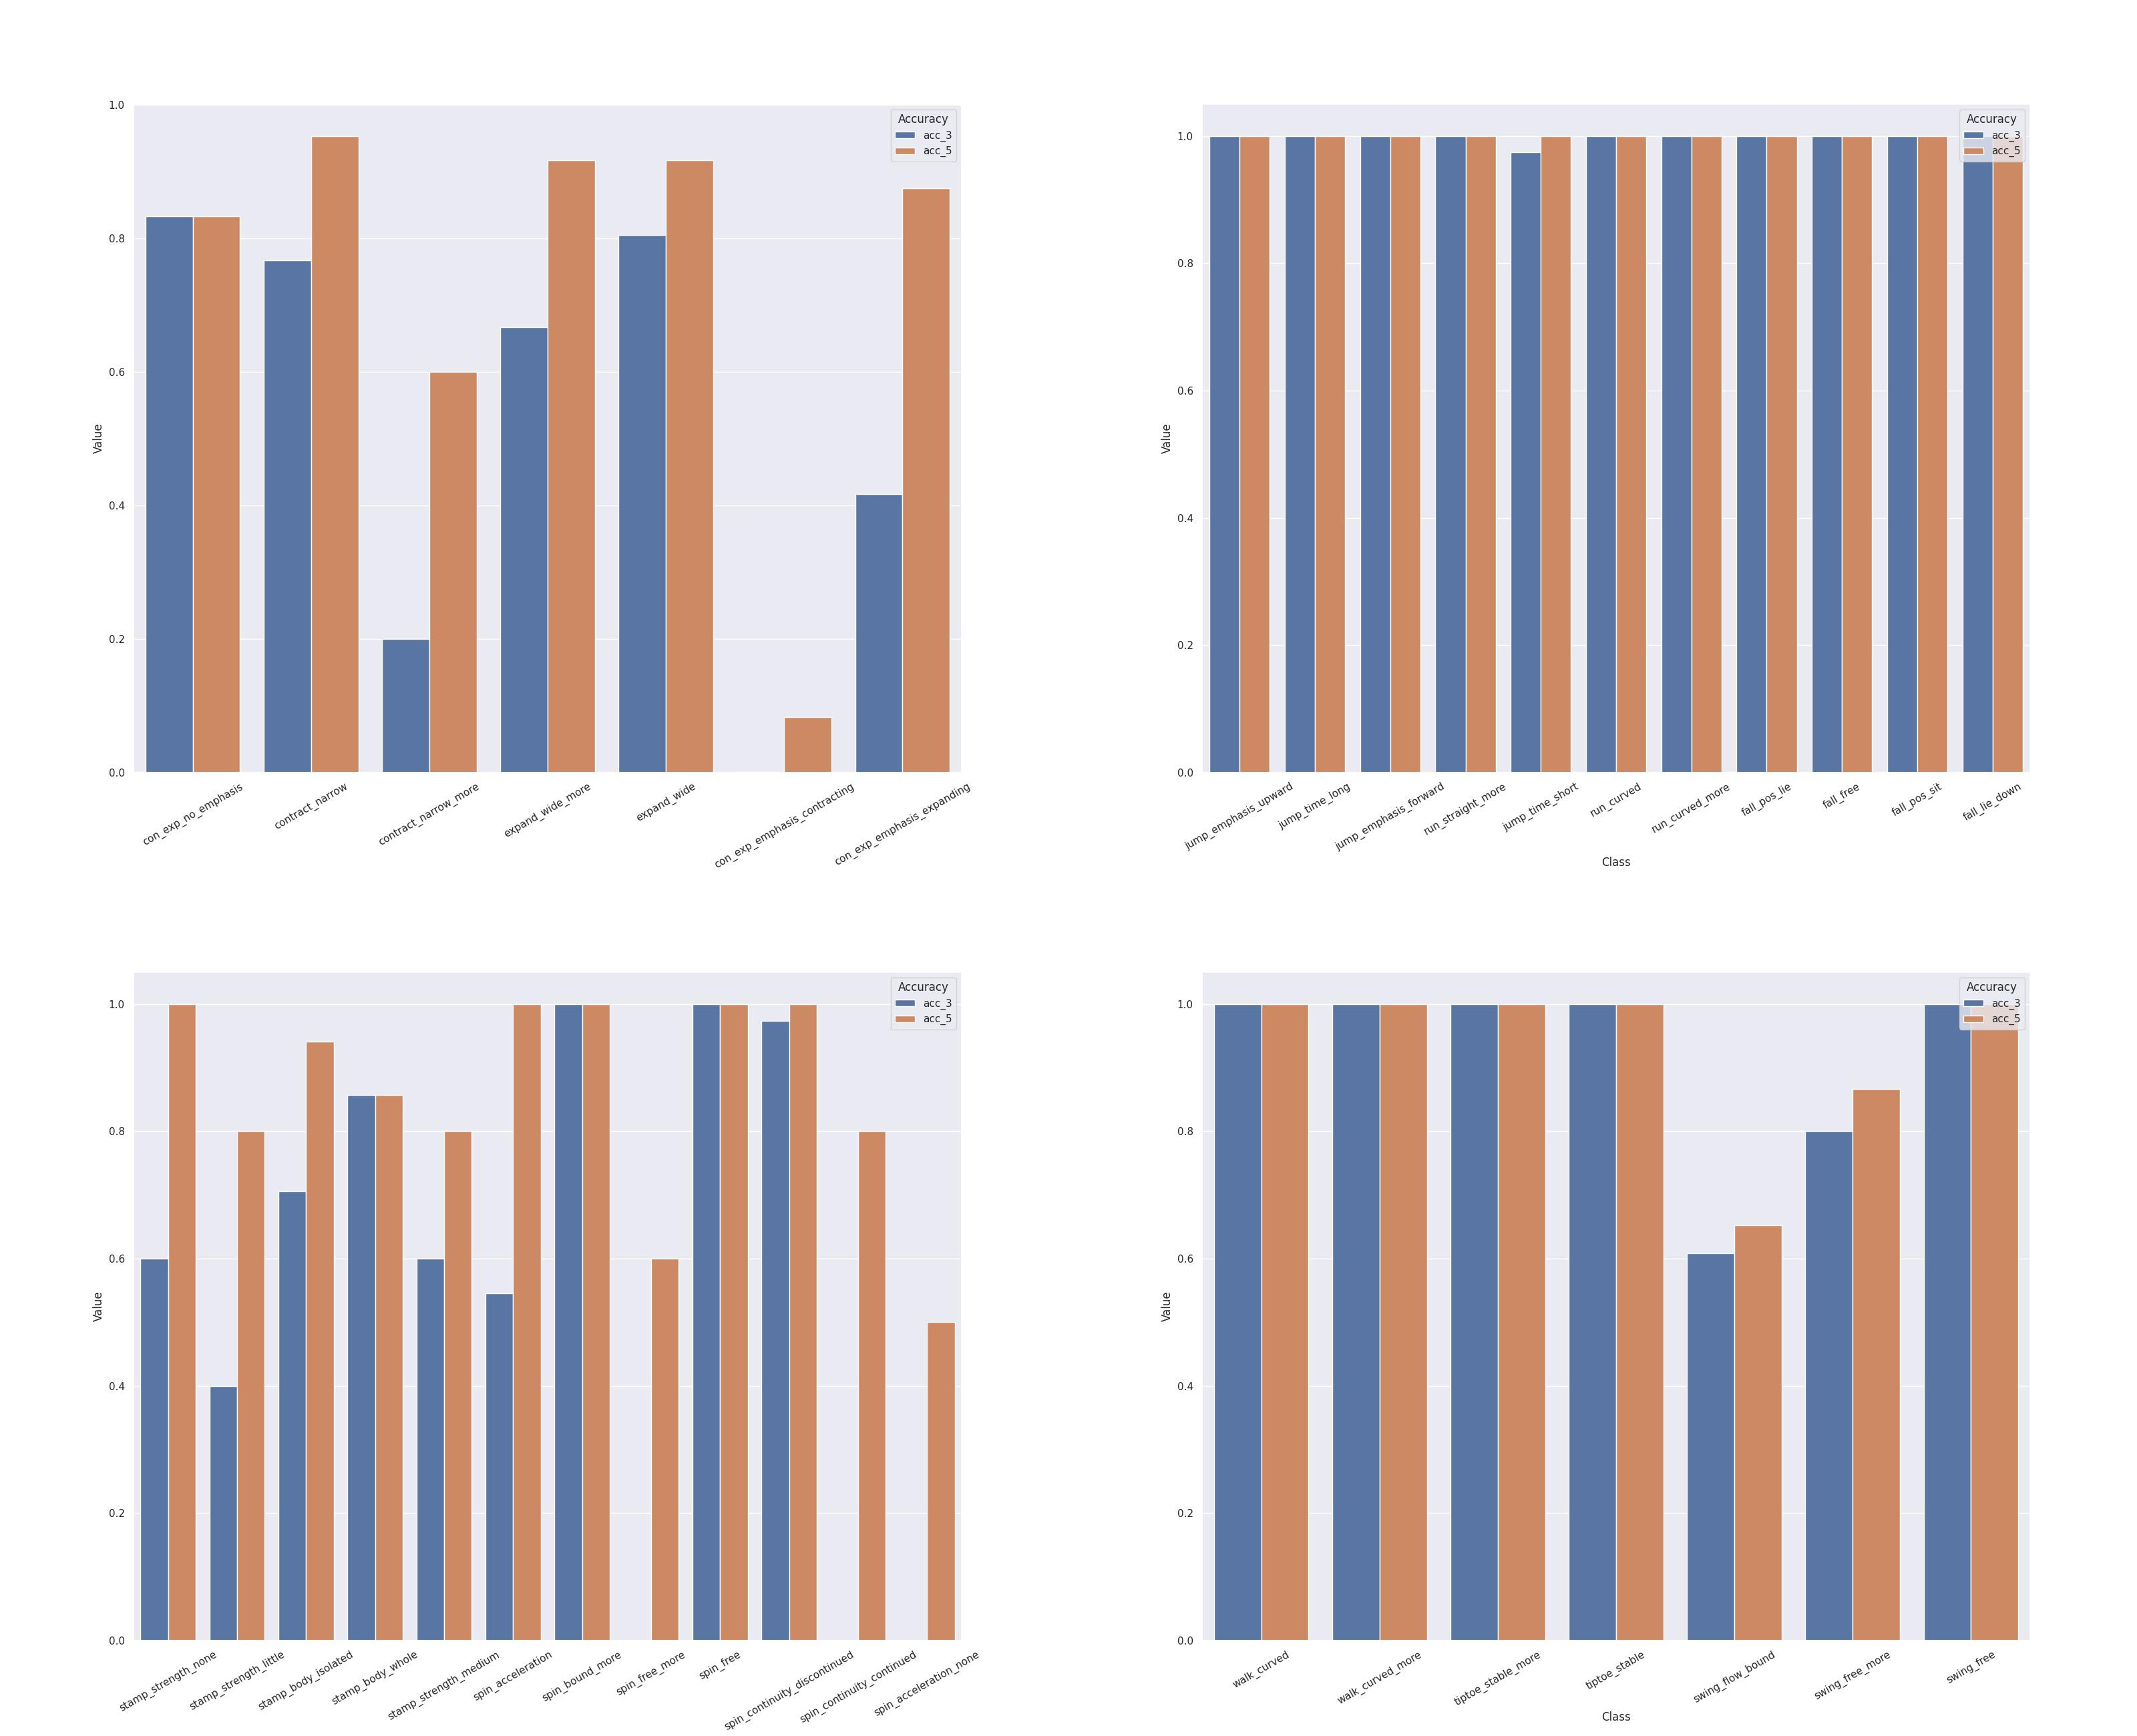
\includegraphics[height={300pt}, width={430pt}]{Thesis/images/acc_per_class_bast_eval.jpg}
\caption{Accuracy for each annotation of the \textit{bast-eval} task for the PoseC3D model pre-trained on the \textit{bast-base} dataset}
\label{fig:acc_per_class_bast_eval}
\end{figure}

\bigskip
\noindent Figure \ref{fig:acc_per_class_bast_eval} shows the \textit{top-3} and \textit{top-5} accuracy for each class of the \textit{bast-eval} dataset for the best performing classifier, namely \textit{PoseC3D-bb-pr-64x1x1-0.6d}. The classifier is able to perfectly classify, with (or almost) 100\% accuracy, the following tasks of this dataset:

\begin{itemize}
    \item all evaluations of jump: \textit{jump-emphasis-upward}, \textit{jump-emphasis-forward}, \textit{jump-time-long}, \textit{jump-time-short}
    \item all evaluations of run: \textit{run-straight-more}, \textit{run-curved}, \textit{run-curved-more}
    \item all evaluations of fall: \textit{fall-pose-lie}, \textit{fall-free}, \textit{fall-pos-sit}, \textit{fall-lie-down}
    \item all evaluations of walk: \textit{walk-curved}, \textit{walk-curved-more}
    \item all evaluations of tiptoe: \textit{tiptoe-stable}, \textit{tiptoe-stable-more}
    \item some evaluations of spin: \textit{spin-bound-more}, \textit{spin-free}, \textit{spin-continuity-discontinued}
    \item one evaluation of swing: \textit{swing-free}
\end{itemize}

\noindent Thus, the model is able to capture 45\% of the annotations perfectly, which is a splendid job considering the discussed difficulties that the \textit{bast-eval} dataset poses as well as the more inferior performance of the other two models, SlowOnly and I3D. Nevertheless, the influence of the imbalanced classes of the dataset is overt in the following tasks:

\begin{itemize}
    \item \textit{emphasis} evaluation of \textit{contract-expand}: the \textit{emphasis-contracting} annotation is barely being picked up even in the \textit{top-5} accuracy. The main reason for this probably is that this evaluation only has 18\% of the total values that the other two evaluations, namely \textit{no-emphasis} and \textit{emphasis-expanding} are taking. There are probably simply not enough samples for the model to properly learn to differentiate this evaluation from the two others, and hence most of the predictions go as false positives in the other two categories.
    \item \textit{kinesphere} evaluation of \textit{contract}: the \textit{contract-narrow} evaluation has more than double the amount of samples than the \textit{contract-narrow-more} has. Thus, this alone could be enough to prime the model into being biased towards the \textit{contract-narrow} evaluation, to the expense of \textit{contract-narrow-more} and hence we get the procured prediction results as shown in the figure. To be fair, the model is picking it up to a certain degree when considering the \textit{top-5} accuracy. Interestingly, the model is able to nicely capture the \textit{kinesphere} evaluation of \textit{expand} even though a roughly similar imbalanced state exists between \textit{expand-wide} and \textit{expand-wide-more}. This is probably due to the fact that the differences between the later states are more pronounced than the subtle differences between the states of \textit{contract}. In other words, the kinesphere while expanding is easier to pick up than the kinesphere while contracting, since in the latter state the body is wide open, and pose estimation is therefore relatively easier than in the former state. The model probably needs more samples for \textit{contract}, while \textit{expand} is learned with relatively few samples because, again, the differences in its state are more conspicuous than the former.
    \item \textit{continuity} evaluation of \textit{spin}: the \textit{discountinued} evaluation has roughly three times as much samples as the \textit{continued} evaluation.
\end{itemize}

\noindent Nevertheless, the model also showed resilience towards some of  the imbalanced classes because it classified imbalanced tasks such as \textit{expand-wide-more} and \textit{expand-wide} or \textit{stamp-body-isolated} and \textit{stamp-body-whole} quite satisfactory. Therefore, we conclude that if the evaluation is not particularly hard, the model can still learn it even though its classes might be imbalanced. However, if the evaluation is hard and its values are imbalanced, the model has a hard time properly classifying it.

All in all, the tasks that presented the most problems were \textit{stamp} and \textit{spin}, while the easiest to learn were \textit{walk}, \textit{run}, \textit{jump}, \textit{fall} and \textit{tiptoe}.

\bigskip \bigskip
\noindent\textbf{Conclusion}: We can conclude that the best suited model for the classification of the \textit{bast-eval} task, as with the previous task, remains \textbf{PoseC3D}. The results achieved by this model look very promising. A crucial component to its success was using a very dense sampling strategy of \textit{$64 \times 1 \times 1$}. Considering that almost half of the annotations were classified perfectly, it should be possible to achieve similar results with the rest of the annotations, given an appropriate dataset. To answer the second research question, yes, it should be possible to automate the BAST evaluation end-to-end and remove the need for a certified evaluator.

\newpage
\subsection{Robustness of Models}
\label{research_question_3}

\fbox{\begin{minipage}{38.5em}
RQ3: How robust are the models trained in the previous two chapters outside the BAST context? For the \textit{bast-base} task, can we use the nine movements as general categories in a dance-like context? For the \textit{bast-eval} dataset, do the evaluations extend in a dancing context?
\end{minipage}}

\bigskip \bigskip
\noindent In the scope of the \textit{vortanz} project, it is desired to investigate whether the nine base annotations of the \textit{bast-base} and 42 annotations of the \textit{bast-eval} datasets can be generalized outside the BAST domain. In other words, can models trained on BAST material recognize these movements in other contexts? For this purpose, two experiments are presented in this section.

The first one consists of testing the models trained on \textit{bast-base}; namely, it was checked if these nine labels can be used as broad categories in other domains. For example, \textit{walk} could be used as a category for slow movements, while \textit{run} for faster ones, while labels like \textit{tiptoe} and \textit{rotate} on the other hand have a clear usage in dancing contexts. For this purpose, and in a loss of any other datasets, these models were tested on the second task of the BAST analysis itself. In this task the participants are asked to emulate with their body movements \textit{water}, \textit{fire}, \textit{air} and \textit{earth}. They are free to pick any movement they would like and are given one minute for each task. While this is not outside the BAST domain, the type of movements that were utilized during these tasks differ widely from the type of movements seen during the first phase of the BAST analysis, from which the two \textit{bast-} datasets were created. This is facilitated by the fact that the subjects are free to pick any movement in their emulations. Hence the second phase of the BAST analysis can serve as a good domain testing context even though it is technically the same domain.

The second experiment then consists of testing the 42 evaluation annotations of the \textit{bast-eval} dataset. For this purpose, a small dataset completely outside the bast context was used. The subjects performed only one action, namely the \textit{kinesphere} in a completely different way from the way it was performed in the first phase of BAST. Hence, we can also consider this dataset a good way to test the domain context and broader generalization of the models.

To conclude, the movements that are performed in these two domain testing datasets are very different from the movements that the model has encountered in the \textit{bast-base} and \textit{bast-eval} datasets. Figures \ref{kinesphere_dataset} and \ref{bast_avatar} give two examples illustrating movements from the \textit{kinesphere} and \textit{bast-avatar} datasets respectively.

\subsubsection{Testing Base Annotations} 
\label{research_question_3_1}

In order to properly test the models trained on \textit{bast-base} we would need an annotated validation dataset. This is not the case with the avatar-videos of the BAST analysis since they were not labeled. For this reason, a general examination of the actions was manually done in order to extract specific properties from them. The idea is to thereafter run the model  on the \textit{bast-avatar} dataset, and compare its predictions with common sense interpretations derived the extracted cues. We can thus draw certain conclusions on the generalization capabilities of the model, although they will admittedly not be very accurate.

The movements to be performed for this task are left up the discretion of each subject; hence the dataset has much variance in the movements that it contains. The tasks can be considered difficult, and many subjects struggle to come up with adequate movements. Indeed, many videos were left out of the analysis simply because subjects got stuck and did not know what movements to perform or performed inferior quality movements. Below, general cues for interpreting the model's results are presented.

\begin{itemize}
    \item \textbf{water}: most subjects represented this by emulating wave patterns with their arms and hands, with the hand movements pointing to the horizontal direction. Many people also performed fish-like movements. For example, some people fell to the ground and imitated how the fish swims.
    \item \textbf{fire}: most people represented this by emulating something going up into the air or imitating explosions by jumping and using their body and hand movements. In contrast to the \textit{water} task, the hand movements in this task point to the vertical, upward direction.
    \item \textbf{air}: represented simply by moving around the room as well moving the hands a lot. Some people also rotated to simulate a whirl.
    \item \textbf{earth}: represented mainly by falling to the ground, and after afterwards moving around the ground on all fours. Some people made rough contracting movements while on the grounds. Others preferred to hit the ground (perhaps rather primed by the first BAST task).
\end{itemize}

\noindent The \textit{bast-avatar} dataset consists of $21$ videos in total. They were further split into 10-second clips, which were then fed to the model for prediction. Table \ref{avatar_analysis_top_1} represents the results after running them through the \textit{posec3d} model. Only the \textit{top-1} accuracy was considered for this analysis. Based on the cues defined above, we can make the following comments on the model's performance for each of the four tasks:

\bigskip
\noindent\textbf{water}: the three most frequent predictions are \textit{walk}, \textit{contract-expand} and \textit{swing-upper-body}. Considering that many subjects were trying to emulate waves with their arm and hand movements, it makes much sense that the model will be predicting both \textit{walk} and \textit{swing-upper-body}. Moreover, \textit{contract-expand} also makes sense because this is the movement that the model assigned to the subjects that were performing fish-like movements. Even thogh many people fell to the ground when performing fish-like movements, the model was more frequently predicting \textit{contract-expand} rather than \textit{fall} for these types of movements. This can be explained by the fact that the \textit{fall} task had far fewer clips than the other tasks during the model's training (see Figure \ref{bast_base_cls_dist}).

\bigskip
\noindent\textbf{fire}: the three most frequent predictions by the \textit{PoseC3D} model for this task are \textit{contract-expand}, \textit{run} and \textit{jump} with the first one being more frequent than all of the rest taken together. This also makes sense when compared with the extracted cues, because the subjects were mostly emulating fire by moving up and down, both with their body as well as their hands. Also, at times the subjects were also running and jumping and the model is also able to correctly capture this. We can conclude that the model is generalizing pretty well for this task.

\begin{figure}[h]
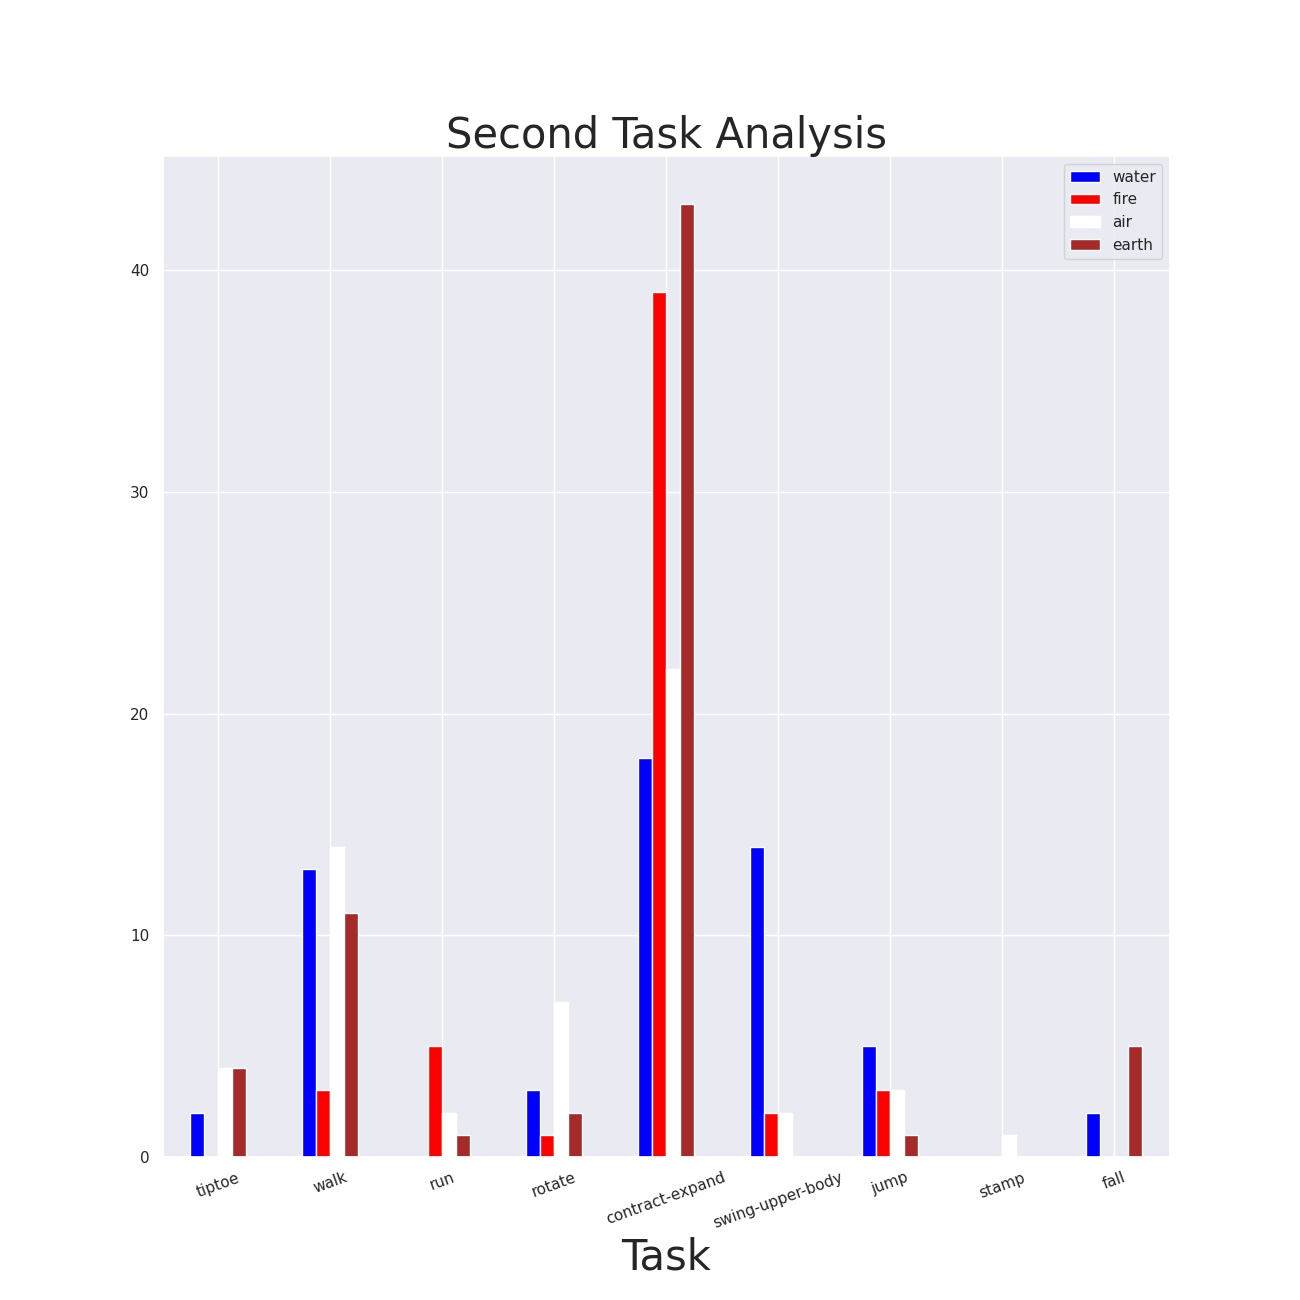
\includegraphics[height={350pt}, width={430pt}]{Thesis/images/avatar_analysis_top_1.jpg}
\caption{Results after testing the base model on the second task of the BAST analysis, the \textit{bast-avatar} dataset}
\label{avatar_analysis_top_1}
\end{figure}

\bigskip
\noindent\textbf{air}: for this task the three most frequent predictions of the \textit{PoseC3D} model are \textit{contract-expand}, \textit{walk} and \textit{rotate}. Given that the subjects were frequently moving around the room with different hand movements, it makes sense that \textit{contract-expand} and \textit{walk} are the top two movements. Admittedly, the interpretation of the hand movements in this task as \textit{contract-expand} is somewhat crude, but it should be kept in mind that the model does not have any better representational categories to represent the subtle differences in different hand movements. That is why it picks up hand movements in all the tasks simply as \textit{contract-expand}. Finally, rotating, which the subjects were frequently performing for this task was also picked up correctly by the model.

\bigskip
\noindent\textbf{earth}: the three most frequent predictions of this task are \textit{contract-expand}, \textit{walk} and \textit{fall}. Most subjects fall to the ground and perform different movements there, such as walking on all four. As seen for the \textit{water} task, when the subjects are on the ground, the model puts the emphasis more on the movements performed rather than the state of falling itself. Therefore the model picks up the movements that the subjects are performing while on the ground and such movements are mostly picked up as \textit{contract-expand}. The stamping on the ground movements were also not properly picked up by the model, rather being interpreted as walking movements. All in all, we can also conclude that the model has a fairly good generalization for this task as well.

\bigskip \bigskip
\noindent\textbf{Conclusion}: Overall, we can say that apart from a slight bias on the \textit{contract-expand} movement (in lack of better annotations), and \textit{fall}, because there are not enough samples, the model is generalizing reasonably well for the \textit{bast-avatar} dataset when compared to the cues presented at the beginning of this section. This generalization should be taken with a grain of salt, however, because the \textit{bast-avatar} dataset did not have ground-truth evaluations.
\bigskip

\subsubsection{Testing Evaluation Annotations}
\label{research_question_3_2}

The \textit{kinesphere} dataset as depicted in Figure \ref{kinesphere_dataset} is a complex one containing movements never seen before by the model. It consists only of one type of movement, namely, the \textit{kinesphere} movement, which is made up by many different types of submovements. The kinesphere in the test dataset deals with the spatial aspects of the personal moving space. It is a derivative of the Laban analysis (see Section \ref{intro_bast_laban}) and concerns the usage of the 360 degree motion's space dealing with all dimensions such as vertical or horizontal. Accordingly three evaluations are defined: 
\begin{itemize}
    \item Narrow kinesphere: movements internal to the body or close to it.
    \item Middle kinesphere: mostly everyday movements. Bent limbs, use of middle joints (e.g. knee or elbow). 
    \item Wide kinesphere: stretched out in such way as to use the maximum possible space. Streching arms and legs as much as possible around all 360 degrees.
\end{itemize}

\noindent The kinesphere evaluation is also part of the \textit{bast-eval} dataset, namely on the \textit{contract-expand} task, as this task can be evaluated in terms of its kinesphere. The evaluations are \textit{narrow}, \textit{wide} and a middle ground between them. These roughly correspond to the above-mentioned annotations of \textit{kinesphere} test dataset. However, the quality of the movements between these two datasets differs widely. Figure \ref{bast_contract_expand} shows the kinesphere as performed in the \textit{bast-eval} dataset. The differences are self-evident when contrasted to Figure \ref{kinesphere_dataset}. On the testing dataset, we have professional dancers performing rich movements to represent the scope of the kinesphere, whereas, in the BAST analysis, we have students performing stiff and mechanical movements to represent this same kinesphere. Actually, the students are not even aware of the three categories of the kinesphere; hence they are not performing them with a view to the kinesphere room usage at all. They are simply performing the \textit{contract-expand} task. Indeed, the purpose of BAST is to let the subject perform the movements as he sees fit without any external influence to observe his psychological state.

For this experiments 7 videos of roughly one-minute length were utilized. As with other experiments, they were split into 10-second clips and feed to a pre-trained \textit{PoseC3D} model on the \textit{bast-eval} dataset. The \textit{top-2} accuracy of each prediction was taken into account. Table \ref{tab:research_question_3_kinesphere} shows the top three most frequent movements that the model predicted for each evaluation of the \textit{kinesphere} test dataset.

\begin{table}[h!]
  \begin{center}
    \caption{\textit{kinesphere} domain-test dataset analysis}
    \label{tab:research_question_3_kinesphere}
    \begin{tabular}{l|c|c|c|c}
      \textbf{Ground truth} & \textbf{Model's prediction} & \textbf{Count}\\
      \hline
      \multirow{3}{*}{narrow kinesphere} & \textit{jump-time-long} & 13\\
       & \textit{stamp-body-isolated} & 12\\
       & \textit{jump-emphasis-upward} & 9\\
       \hline
       \multirow{3}{*}{middle kinesphere} & \textit{jump-time-long} & 7\\
       & \textit{con-expand-no-emphasis} & 7\\ 
       & \textit{walk-straight-more} & 6\\ 
        \hline
       \multirow{3}{*}{wide kinesphere} & \textit{stamp-strength-none} & 9\\
       & \textit{stamp-body-isolated} & 6\\ 
       & \textit{jump-time-long} & 6\\ 
    \end{tabular}
  \end{center}
\end{table}

\noindent It is very clear that the model is unable to generalize for the \textit{kinesphere} dataset, and that its performance is unsatisfactory. Three remarks can be made:

\begin{itemize}
    \item The four expected movements of the \textit{bast-eval} task, namely \textit{expand-narrow}, \textit{expand-wide}, \textit{expand-wide-more} and \textit{expand-narrow-more} did not come up at all.
    \item The model is outputing movements that are not related to the kinesphere task. For example, the top prediction for \textit{narrow-kinesphere} and \textit{middle-kinesphere} is \textit{jump-time-long}.
    \item There are no subtle differences between the predictions of the model for \textit{narrow-kinesphere}, \textit{middle-kinesphere} or \textit{wide-kinesphere}, i.e. the model outputs the same or similar predictions in all three of them and cannot differentiate them.
\end{itemize}

\bigskip
\bigskip
\noindent\textbf{Conclusion}: For the two experiments performed in this chapter, we can say that the first one can demonstrate that the categories of the \textit{bast-base} dataset could be potentially extended to other domains. On the other hand, the categories of \textit{bast-eval} seem unlikely to be extended to other domains as they are very specific to the BAST analysis. However, both conclusions are not conclusive because in the first case, an annotated evaluation dataset was missing, and in the second case, there were not enough data to train robust models based on the \textit{bast-eval} dataset in the first place. Future research could further investigate these two points.

\newpage
\subsection{Transfer Learning}
\label{research_question_4}

\fbox{\begin{minipage}{38.5em}
RQ4: How important is transfer learning for classiying both the \textit{bast-base} and \textit{bast-eval} tasks? Which benchmark dataset yields the most benefits in transfer learning? How beneficial is it to use the \textit{bast-base} dataset as pre-training for \textit{bast-eval}?
\end{minipage}}

\bigskip \bigskip

\noindent As already examined in Sections \ref{insufficient_data} and \ref{imbalance_data}, we have an insufficient data problem for both our datasets, which is more pronounced for the \textit{bast-eval} dataset. We also have an imbalanced dataset problem for the \textit{bast-eval} only. In the aforementioned sections, it was proposed to use transfer learning to ameliorate and tackle these problems. Therefore, this chapter examines transfer learning and its benefits in great detail. 

First, Section \ref{research_question_4_1}, compares training 3D models from scratch with initializing them first with weights from other datasets. Next, Section \ref{research_question_4_2} examines the benefits of using weights from different benchmark datsets, and specifically tries to pinpoint which is the best benchmark dataset for which task and model architecture. Section \ref{research_question_4_3} then examines the differences between benchmark and \textit{bast-base} transfer learning for the \textit{bast-eval} task. Finally, Section \ref{research_question_4_4} shows how a pre-training with \textit{bast-base} solves, to a certain degree,  the class imbalance problem of the \textit{bast-eval} task.

\subsubsection{Tranining From Scratch vs. Transfer Learning}
\label{research_question_4_1}

This section expands upon Section \ref{insufficient_data} and examines the difference between training the models from scratch and initializing them with the weights from benchmark datasets. The idea behind this is to solve the insufficient data problem of both the \textit{bast-base} as well as \textit{bast-eval} dataset because we initialize our models with weights from models pre-trained on quite comprehensive datasets in the HAR domain. Moreover, this could also majorly help with the imbalanced classes problem of the \textit{bast-eval} task. Table \ref{tab:research_question_4_1} shows the results of these experiments.

\begin{table}[h!]
  \begin{center}
    \caption{Training from scratch vs. transfer learning}
    \label{tab:research_question_4_1}
    \begin{tabular}{l|l|c|c|}
      \textbf{Model} & \textbf{Task type} & \textbf{Transfer learning} & \textbf{No transfer learning}\\
      \hline
      \multirow{2}{*}{I3D} & \textit{bast-base} & 96.3\% & 87\% \\
        & \textit{bast-eval} & 60\% & 51\%\\
       \hline
       \multirow{2}{*}{SlowOnly} & \textit{bast-base} & 97.31\% & 90.78\% \\
        & \textit{bast-eval} & 71\% & 29.31\%\\
        \hline
        \multirow{1}{*}{SlowFast} & \textit{bast-base} & 96\% & 89.8\% \\
       \hline
       \multirow{2}{*}{PoseC3D} & \textit{bast-base} & 97.27\% &  95.9\%\\
        & \textit{bast-eval} & 77.39\% &  72.19\%\\
       \hline
    \end{tabular}
  \end{center}
\end{table}

\bigskip
\noindent For the first three models, namely I3D, SlowOnly, and SlowFast, using weights from benchmark datasets results in tremendously huge benefits. The gains were as much as $9.3\%$ for the SlowFast model on the \textit{bast-base} task and as much as $40\%$ for the SlowOnly model on the \textit{bast-eval} task. Without pre-training, these models tend to converge very fast and are therefore unable to improve. This suggests that transfer learning is indispensable for both BAST tasks and is able to solve the insufficient dataset problem. In other words, although the quality of the BAST dataset is meager, we can ameliorate this problem to a great extend by utilizing already initialized models on benchmark datasets in the field. For the PoseC3D model on the other hand, the benefits are more modest, namely $2.3\%$ and $5\%$ for the \textit{bast-base} and \textit{bast-eval} datasets respectively. This further serves to enforce the dominance of PoseC3D over other 3D ConvNets since it is able to learn strong models even when trained from scratch. Nevertheless, the gains in accuracy when using pre-trainings in PoseC3D are also quite significant. Especially for the \textit{bast-eval} dataset, a $5\%$ boost in accuracy is very helpful.

\subsubsection{Transfer Learning With Various Benchmark Datasets}
\label{research_question_4_2}

Having established the benefits of transfer learning, this section examines the effect that pre-training on various benchmarks has on the models' performance. Specifically, it would be useful to know, which benchmark dataset results in the highest accuracy gains for which BAST task. Experiments were performed with the SlowOnly, TIN, and PoseC3D models. The benchmark datasets considered are: \textit{omni-sourced}, \textit{kinetics-400}, \textit{sth-sth-v2}, \textit{gym}, both versions of \textit{ntu}, \textit{hmdb}, and finally \textit{ufc}. Table \ref{tab:research_question_4_2} below presents the results.

\begin{table}[h!]
    \begin{center}
    \caption{Training with various benchmarks for both tasks}
    \label{tab:research_question_4_2}
    \begin{tabular}{l|l|c|c|c}
      \textbf{Model} & \textbf{Benchmark} & \textbf{Bast-Base} & \textbf{Bast-Eval}\\
      \hline
       \multirow{2}{*}{SlowOnly} & Omni-Sourced & 97.31\% & 29.3\% \\
       & Kinetics400 & 24.07\% & 46.4\%\\
       \hline
       \multirow{2}{*}{TIN} & Sth-Sth-V2 & 19.7\% & -\\
       & Kinetics400 & 28.45\% & -\\
       \hline
       \multirow{5}{*}{PoseC3D} & Gym & 96.93\% & 74\% \\
       & Ntu-60 & 95.5\% & -\\
       & Ntu-120 &  96.25\% & 75.7\%\\
       & Kinetics-hmdb &  97.27\% & 72.19\%\\
       & Kinetics-ufc &  97.42\% & 71.36\%\\
       \hline
    \end{tabular}
  \end{center}
\end{table}

\noindent For the SlowOnly model, the best results for the \textit{bast-base} task were achieved with an \textit{omni-sourced} pre-training, while for the \textit{bast-eval} task they were achieved from a \textit{kinetics400} pre-training. This reversing seems very interesting but it was not further tested. For the TIN model, which is a 2D model and was hence only tested on the \textit{bast-base} dataset, the \textit{kinetics400} dataset achieved the best results. Finally, for PoseC3D, for the \textit{bast-base} dataset, the best results were achieved using a \textit{kinetics} and \textit{ucf} training, while for the \textit{bast-eval} dataset were achieved using a \textit{ntu-120} pre-training. Even though the \textit{gym} dataset consists of fine-grained actions as a dataset, and it was speculated that this would help the \textit{bast-eval} task (see Section \ref{fine_gym}), in the end the best performing dataset was \textit{ntu-120}.

\noindent In the next section, we examine the differences between using a benchmark dataset and using the \textit{bast-base} dataset as pre-trainings for the \textit{bast-eval} task.

\subsubsection{Transfer Learning With the Base Task for the Eval Task}
\label{research_question_4_3}

This section poses the question as to how useful a pre-training with the \textit{bast-base} task is for the \textit{bast-eval} task. Specifically, now that we know that transfer learning using benchmark datasets is indispensable for the tasks at hand, the question would be whether a pre-training with \textit{bast-base} is more helpful for the \textit{bast-eval} task than a simple pre-training with a benchmark dataset is. The idea is, as elaborated in Section \ref{initial_analysis_bast_eval}, that since the latter consists of evaluations of the former, having previous knowledge on the coarse-grained categories of \textit{bast-base} could help identify the fine-grained categories of \textit{bast-eval}. Moreover, the models trained on \textit{bast-base} would already have been trained on other benchmark datasets. Thus, we could get the best of both worlds: benchmark datasets as well as pre-training on the \textit{bast-base} dataset. Table \ref{tab:research_question_4_3} below presents the results of the experiments.

\begin{table}[h!]
  \begin{center}
    \caption{Benchmark dataset vs \textit{bast-base} dataset pre-training for the \textit{bast-eval} task}
    \label{tab:research_question_4_3}
    \begin{tabular}{l|l|c|c|}
      \textbf{Model} & \textbf{Benchmark} & \textbf{Bast-base}\\
      \hline
      \multirow{1}{*}{I3D} & 59.5\% & 62.3\% \\
       \hline
       \multirow{1}{*}{SlowOnly} & 60.3\% & 70\% \\
       \hline
       \multirow{1}{*}{PoseC3D} & 75.7\% &  77.39\%\\
       \hline
    \end{tabular}
  \end{center}
\end{table}

\noindent To be fair, the comparison is done only with those experiments that used the same sampling strategy. For example, I3D pre-trained with \textit{kinetics} achieved a good accuracy with the $48 \times 3 \times 1$ sampling strategy but its counterpart with \textit{bast-base} pre-training was trained on a $32 \times 1 \times 1$ sampling strategy. Therefore we compare it to I3D pre-trained on the \textit{kinetics} dataset with the selfsame dense sampling strategy. All the models trained on \textit{bast-base} were initially pre-trained on other benchmark datasets. Thus by pre-training with the \textit{bast-base} dataset for the \textit{bast-eval} dataset we are also indirectly pre-training with some other benchmark datasets.

Results show that pre-training with the \textit{bast-base} dataset brings considerable improvements for the \textit{bast-eval} task. The accuracy is up $~3\%$ in the case of I3D and $~10\%$ in the case of SlowOnly. In the case of PoseC3D it is up a more modest $2\%$. Hence the conclusion is that a pre-training on the \textit{bast-base} dataset is more desirable than a simple pre-training on benchmark datasets for the \textit{bast-eval} task. Next we turn our attention to whether such pre-training can help solve the class-imbalance problem as laid down in Section \ref{initial_analysis_bast_eval}.


\subsubsection{Transfer Learning and Class Imbalance}
\label{research_question_4_4}

The \textit{bast-eval} dataset suffers from a two-fold problem: first, as already mentioned, there are not sufficient samples for its classes, and second these classes are imbalanced. As already investigated and concluded in the previous sections, pre-training with various benchmark datasets solves the insufficient samples problem to a great extend. The remaining problem now is the imbalanced classes. This section tests the theory proposed in Section \ref{imbalance_data}, namely can a pre-training on the \textit{bast-base} dataset ameliorate the imbalanced classes of the \textit{bast-eval} task. For this purpose we compare the accuracy for each class of the \textit{bast-eval} task with and without a pre-training on the \textit{bast-base} task. Figure \ref{fig:acc_per_class_bast_eval} illustrates this for the PoseC3D model pre-trained on the \textit{bast-base} task and Figure \ref{fig:acc_per_class_bast_eval_ntu} illustrates this for the PoseC3D model only pre-trained on the \textit{ntu-120} dataset. 

\begin{figure}[h]
\center
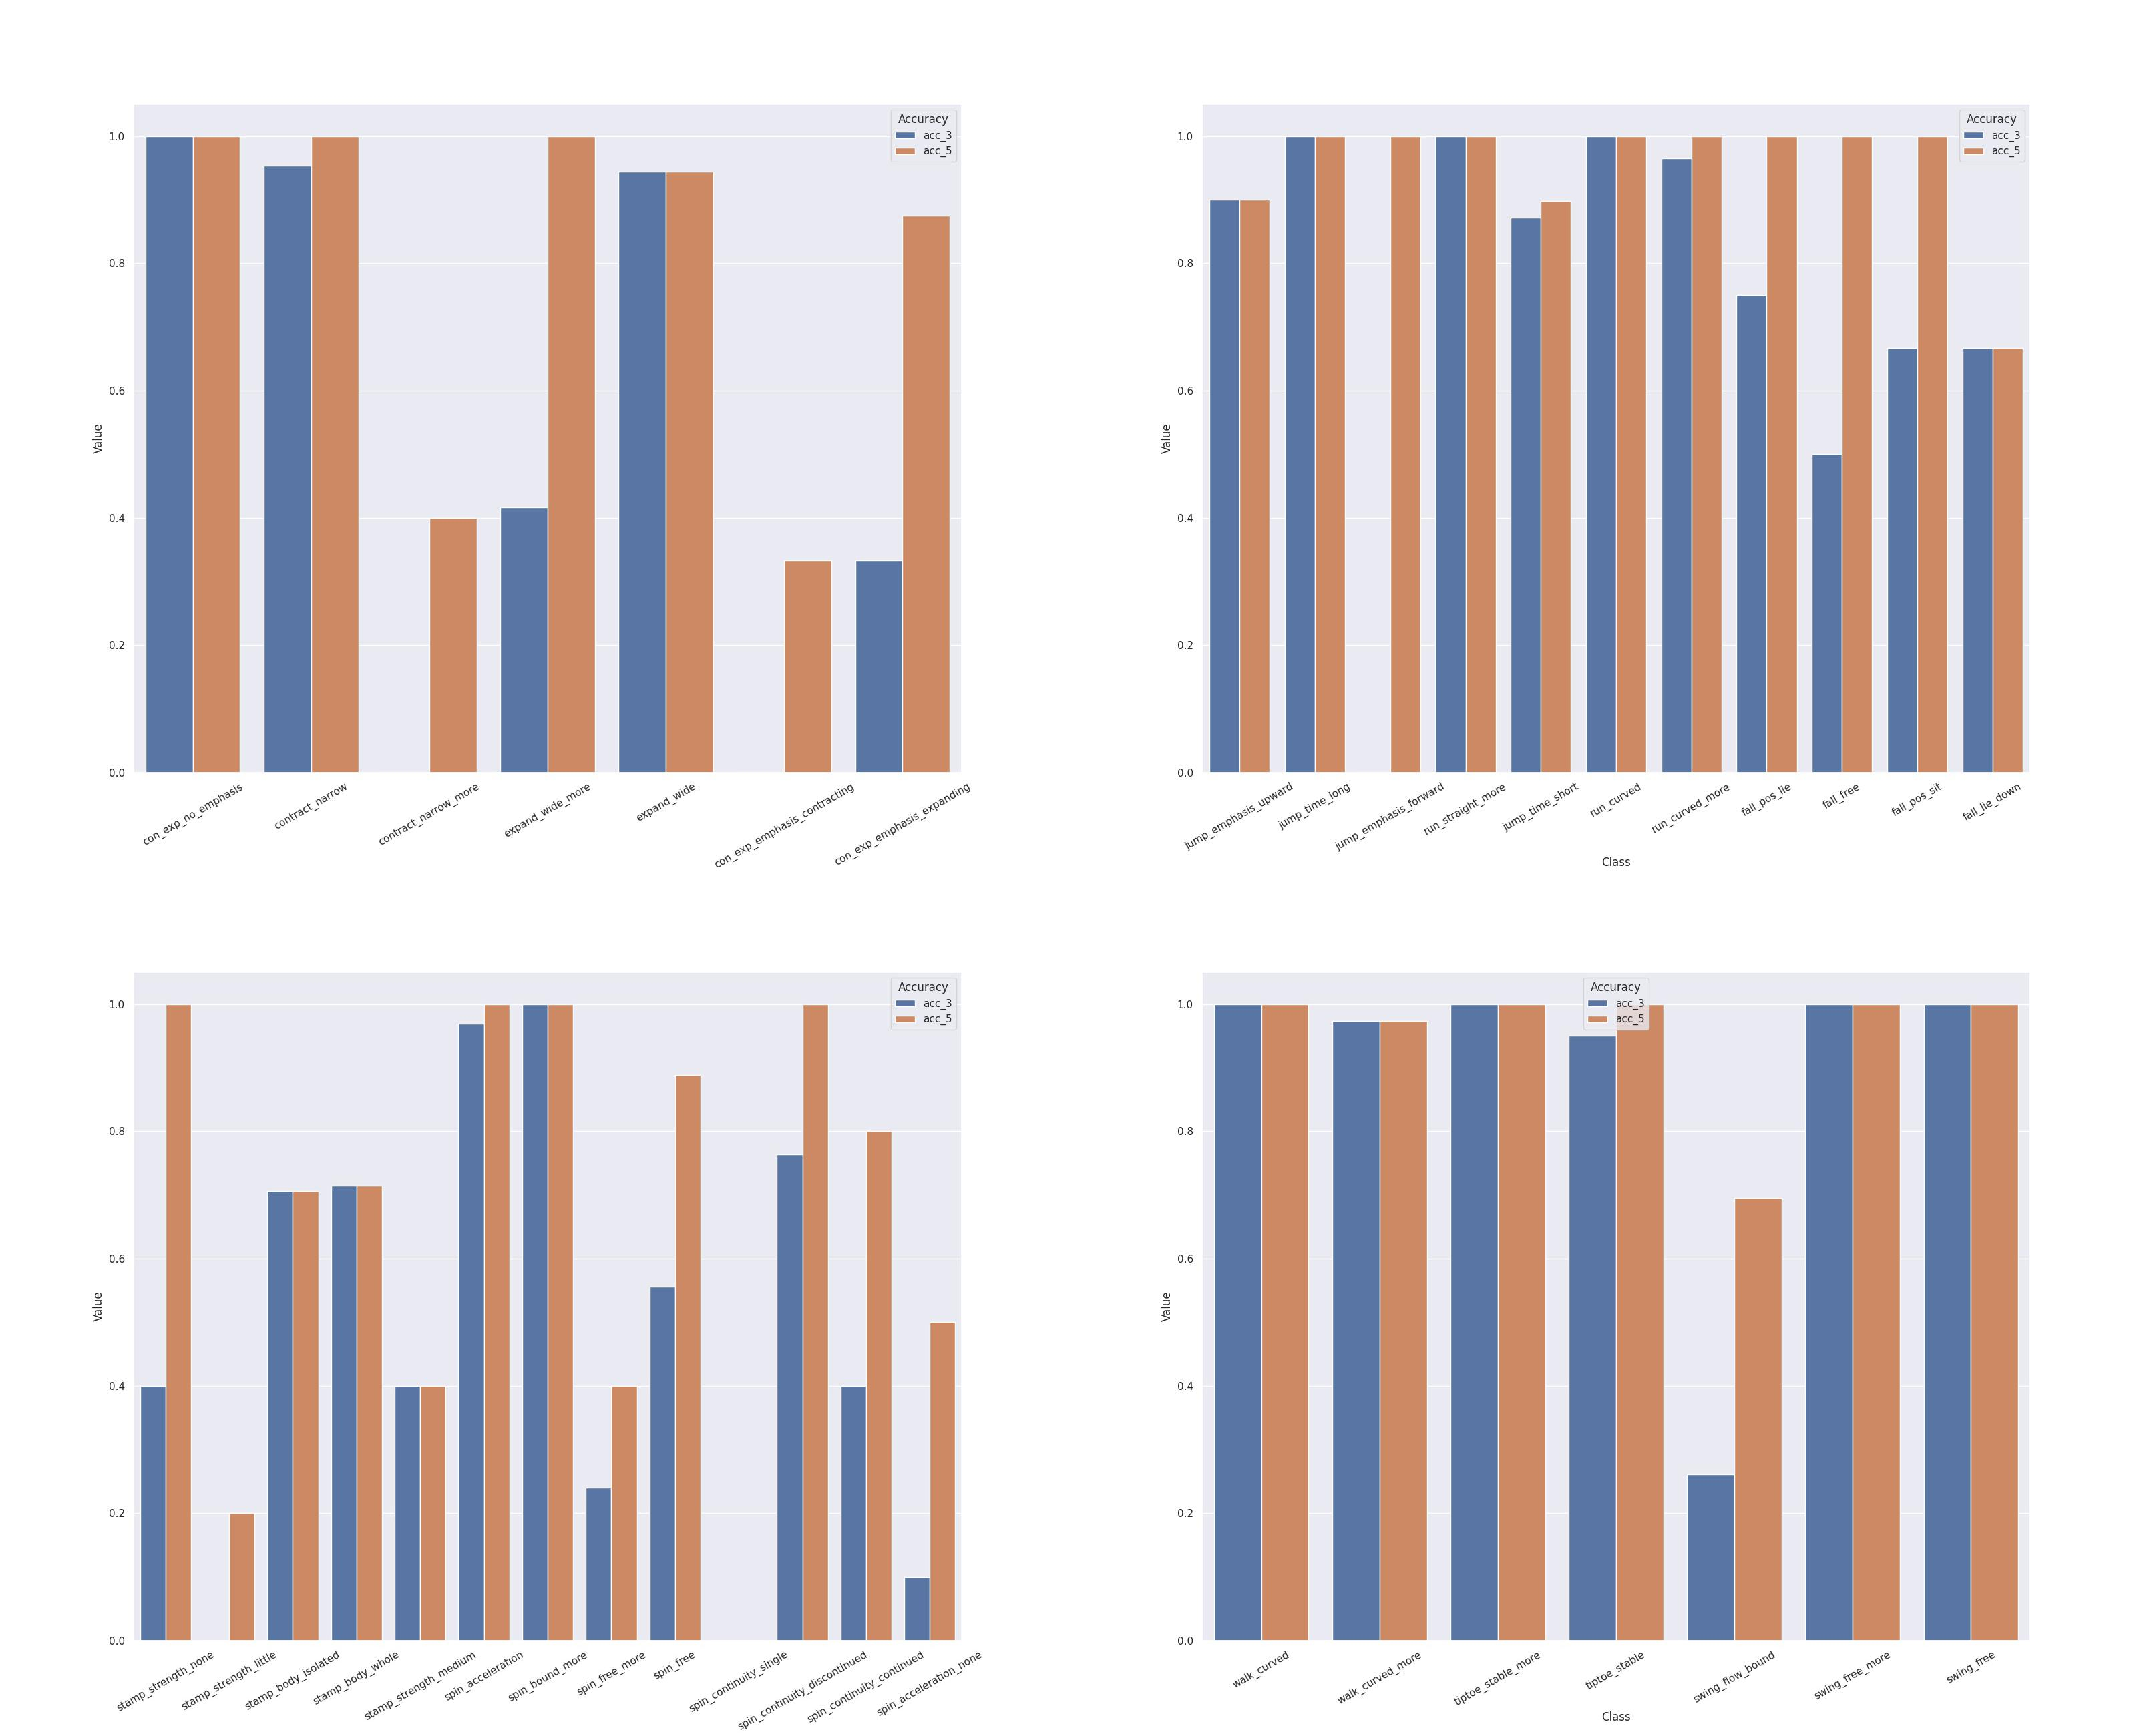
\includegraphics[height={300pt}, width={430pt}]{Thesis/images/posec3d_eval_ntu-120.jpg}
\caption{Accuracy for each annotation of the \textit{bast-eval} task for the PoseC3D model pre-trained on the \textit{ntu-120} dataset}
\label{fig:acc_per_class_bast_eval_ntu}
\end{figure}

\bigskip
\noindent The \textit{top-3} accuracy of the models is \textit{77.39\%} and \textit{75.7\%} respectively. This meager difference of $2.5\%$ in the performance of the trained models and the fact that we are utilizing the same architecture, namely PoseC3D, ensures a robust and fair comparison between the two models, since the only variable remains the pre-training. A close examination of both figures reveals that yes, indeed, the pre-training on the \textit{bast-base} dataset helps solve the imbalanced classes problem of the \textit{bast-eval} dataset. The following points are observed:

\begin{itemize}
    \item the \textit{kinesphere} evaluation of \textit{contract} is imbalanced as the evaluation \textit{contract-narrow} has more than double the amount of annotations that \textit{contract-narrow-more} has. In Figure \ref{fig:acc_per_class_bast_eval_ntu} it is observed that the model is unable to correctly classify this evaluation. The \textit{top-3} accuracy for the \textit{contract-narrow-more} annotation is 0, while the classification of \textit{contract-narrow} is almost perfect. In contrast, in Figure \ref{fig:acc_per_class_bast_eval} we can see that the model has started to recognize the \textit{contract-narrow-more} evaluation.
    \item the \textit{kinesphere} evaluation of \textit{expand} is imbalanced as the evaluation \textit{expand-wide} has more than triple the amount of annotations that \textit{expand-wide-more} has. The accuracy of \textit{expand-wide-more} is roughly $40\%$ for the PoseC3D model trained on \textit{ntu-120} but with a \textit{bast-base} pre-training this accuracy rises to almost $70\%$. Thus the latter model is able to recognize both the classes properly even though they are severely imbalanced.
    \item the \textit{emphasis} evaluation of \textit{jump} is in particular severely imbalanced because the evaluation \textit{jump-emphasis-upward} has as much as eight times more samples than its counterpart \textit{jump-emphasis-forward}. Notwithstanding this, the model pre-trained on \textit{bast-base} is able to perfectly classify both of them when taking into account the \textit{top-3} accuracy. However, the model not pre-trained on \textit{bast-base} cannot even classify one sample correctly when considering the \textit{top-3} accuracy for the \textit{jump-emphasis-forward} evaluation. This is understandable given the severe imbalance but the fact that a pre-training with \textit{bast-base} solves this problem perfectly really serves to prove the point of this section.
    \item the \textit{strength} evaluatuion of \textit{stamp} is slightly imbalanced because \textit{stam-strength-medium} has almost the same amount of annotations as \textit{stamp-strength-none}, and \textit{stamp-strength-little} taken together. For the model not pre-trained on \textit{bast-eval}, the \textit{top-3} accuracy for \textit{stamp-strength-none} is $40\%$ and for \textit{stamp-strength-little} is $0\%$. The model pre-trained on \textit{bast-base} on the other hand has a confidence of $60\%$ and $40\%$ respectively.
\end{itemize}

\bigskip
\noindent To conclude this research question, it was shown that transfer learning is an essential strategy for the task at hand and that the two most suitable benchmark datasets for this purpose are \textit{kinetics} and \textit{omni-sourced}. This solves the class-imbalance problem to a great degree. For the \textit{bast-eval} task, it was shown that pre-training with the \textit{bast-base} task produced more robust and resilient models, especially to the imbalanced classes of this task.

\newpage
\subsection{Background Influence}
\label{research_question_5}

\fbox{\begin{minipage}{38.5em}
RQ5: What role does the background play in the model's performance? How does the models' performance fare if we strip the background from each video? How does this compare to skeleton-based models?
\end{minipage}}

\bigksip
\bigskip
\noindent As already discussed in the introduction to this thesis, A.I. in computer vision generally suffers from the background, different light variations as well as occlusions influences. This is especially the case with human action recognition (HAR) models \cite{pareek2021survey}. If left unchecked, and in the most extreme cases, they can produce biased models, where the output depends on the background rather than the action itself. In this chapter, the influence of the background on the model's performance is studied. Ideally, we would want the model to focus solely on the human inside the frame when deciding about the type of action that is being performed. In other words, models should be robust in that their predictions should not be influenced so much by the type of background that the videos have. This ensures robustness in production.

First, a preliminary analysis of the background influence on HAR models is given in Section \ref{research_question_5_1}. After that, the influence of the background is visually shown using GradCAM heatmaps in Section \ref{research_question_5_2}. Next, models trained with clips stripped of the background are presented in Section \ref{research_question_5_3}. Finally, comparisons with skeleton-based models are presented at Section \ref{research_question_5_4} and conclusions are drawn.

\subsubsection{Preliminary Background Analysis}
\label{research_question_5_1}

To examine the influence of background on the task at hand, an I3D model pre-trained on \textit{imagenet} and the \textit{kinetics} dataset was used. This will also serve to illustrate the influence that the background has on HAR models in general. For this experiment, the gym background of the original clip was striped and replaced with a vineyard background. A kinetics pre-training was used because the \textit{kinetics} dataset has $400$ annotations, including different dance types, which ensures a good range of choices for the model. The I3D model was not fine-tuned on the \textit{bast-base} or \textit{bast-eval} datasets but was instead used raw with its original weights coming from pre-training with the two aforementioned datasets. 

Figure \ref{fig:background_change_influence} illustrates the two different clips that were fed to the model. The image on the left depicts the usual BAST setting inside the gym and the one on the right depicts the subject with a vineyard background.

\begin{figure}[h]
\center
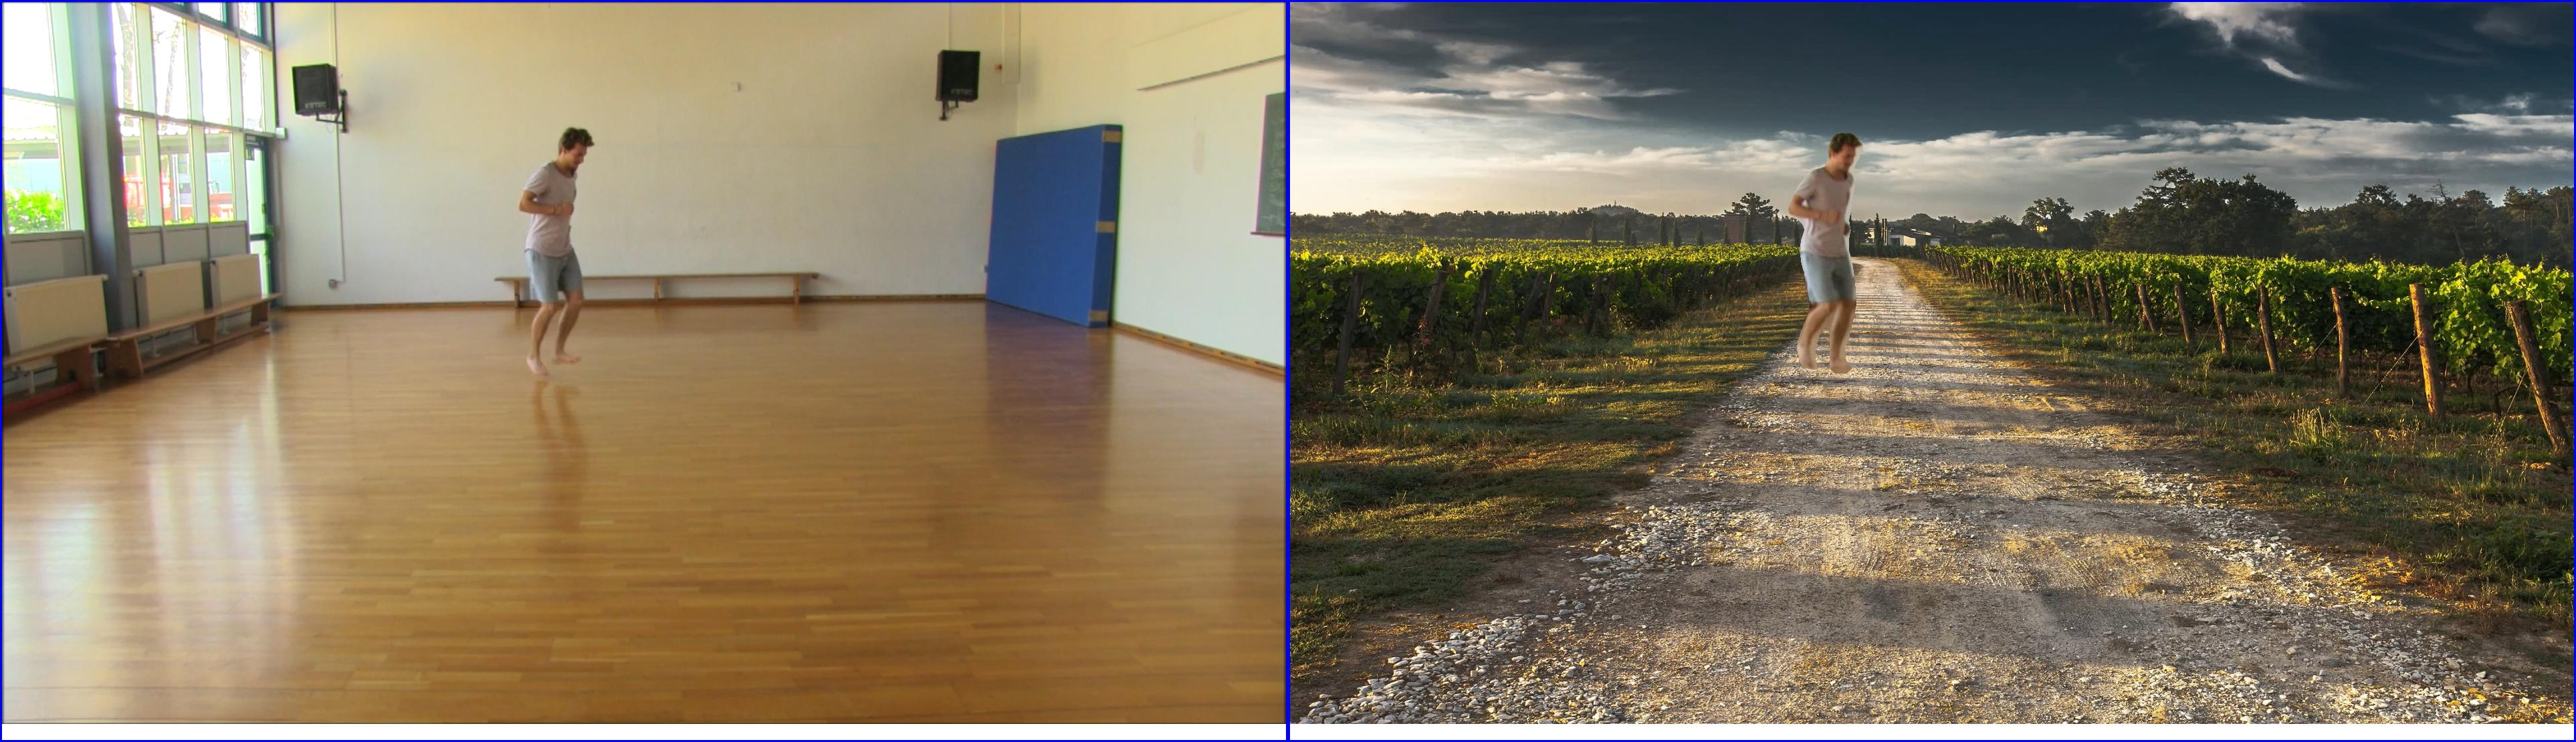
\includegraphics[height={130pt}, width={400pt}]{Thesis/images/background_influence_1.jpg}
\caption{Testing the influence that changing the background has in the model's prediction}
\label{fig:background_change_influence}
\end{figure}

\bigskip
\noindent The predicted results differed drastically. For the first clip, with a gym background, the model predicted \textbf{dancing ballet}, whilst for the second clip, with a vineyard background, the model predicted \textbf{jogging}. A superficial examination of the clips that are marked as dancing ballet from the \textit{kinetics} dataset reveals that such clips are actually performed in closed settings, frequently even inside a gym. On the other hand, the vineyard background consists of an open setting, where jogging usually happens. Hence the model classified the first one as \textit{dancing ballet} because it had a gym background and the second as jogging because it had a background in an open field. This example clearly shows that the model's prediction was influenced more by the type of background and not so much by the actions being performed. However, it should be kept in mind that the model's confidence on these predictions was very low and that the model was not fine-tuned on our specific datasets. This, again, serves to show how easily HAR models can be influenced by such conditions as the background if not trained with an adequate amount of samples.

\subsubsection{GradCAM Analysis}
\label{research_question_5_2}

This section looks at the precise influence that the background has on the model's predictions. We can do this by using the GradCAM model, which visualizes heatmaps of the critical regions in the image that influenced the model in its predictions. Following, results are presented for 2D and 3D models.

\begin{figure}[h]
\center
\includegraphics[height={230pt}, width={370pt}]{Thesis/images/GradCAM_i3d.jpg}
\caption{GradCAM results for the \textit{I3d} model}
\label{fig:GradCAM_i3d}
\end{figure}

\bigskip
\noindent\textbf{3D Models}: Figures \ref{fig:GradCAM_i3d} and \ref{fig:GradCAM_slow_only} present the GradCAM results for the I3D and SlowOnly-omni models respectively. At times, both models perfectly capture the person in the frame. However, we can see that they also struggle with pinpointing and focusing on this person at other times. In general, SlowOnly seems to be faring better at capturing the person on the frame, which makes sense considering its superior performance to I3D. We can also see an overt influence of the background towards the model's final decision. There are even frames where the model is missing the person entirely and focusing just on the background. Given that the background of the datasets always consists of a gym setting, the influence of the background could make it harder for the model to generalize for other types of backgrounds in production.

\noindent In conclusion, for 3D models, the background influences the model's predictions to a certain extend, although not so heavily as is the case for the 2D models (presented below).

\begin{figure}[h]
\center
\includegraphics[height={230pt}, width={370pt}]{Thesis/images/GradCAM_slow_only.jpg}
\caption{GradCAM results for the \textit{SlowOnly-omni} model}
\label{fig:GradCAM_slow_only}
\end{figure}

\bigskip
\noindent\textbf{2D Models}: Figure \ref{fig:gradcam_2d} shows the GradCAM results for two 2D models, namely \textit{Tanet} and \textit{Tsn}. We can see that the former is learning much better than the latter, where the activations seem to be very weak. Indeed, \textit{Tsn's} performance is so weak that even the background is not being activated, and hardly anything at all is visible. \textit{Tanet} on the other hand, is faring relatively good and has a somewhat comparable performance to the above-shown 3D models. All in all, we conclude that 2D models are more sensitive to background influences.

\bigskip
\noindent In the next section, we examine how the models fare when the background is altogether stripped. Could this ameliorate to a certain extent the background influence on the model's predictions?

\begin{figure}[h]
\center
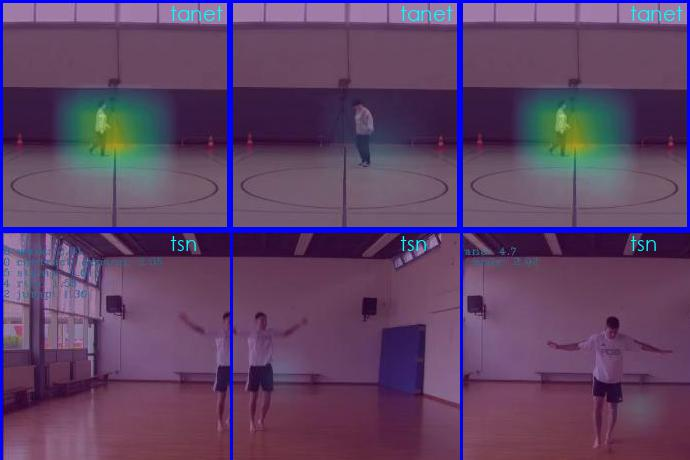
\includegraphics[height={230pt}, width={370pt}]{Thesis/images/gradcam-2D.jpg}
\caption{GradCAM results for the \textit{Tanet} (up) and \textit{Tsn} (below) models}
\label{fig:gradcam_2d}
\end{figure}

\subsubsection{Stripping the Background}
\label{research_question_5_3}

This section presents the results for models trained on a blank background. The background of all the clips was stripped and replaced with a white background as shown in Figure \ref{fig:fall_no_background}. The process is as follows. First, each frame is extracted from the video. Then, salient object detection using \textit{u2net} is performed on each of the extracted frames \cite{qin2020u2}. After that, a bitwise subtraction is performed between the \textit{u2net} result and the original frame. This highlights the person in the frame while also ensuring a more robust result in the end. Finally, from the bitwise subtraction output, every black pixel is replaced with a white one, and the detected salient object is kept as it is. The frames are then stacked together in their original order to form the clip. 

The result of the salient object detector is not perfect. For example, in some cases, the head was missing for some frames during some of the clips. Although the gym room is pretty much empty, at times, the \textit{u2net} model also picked up some minor objects such as a speaker or traffic cone in the background. Thus, while the process is not perfect, it is good enough for our purposes.

\begin{figure}[h]
\center
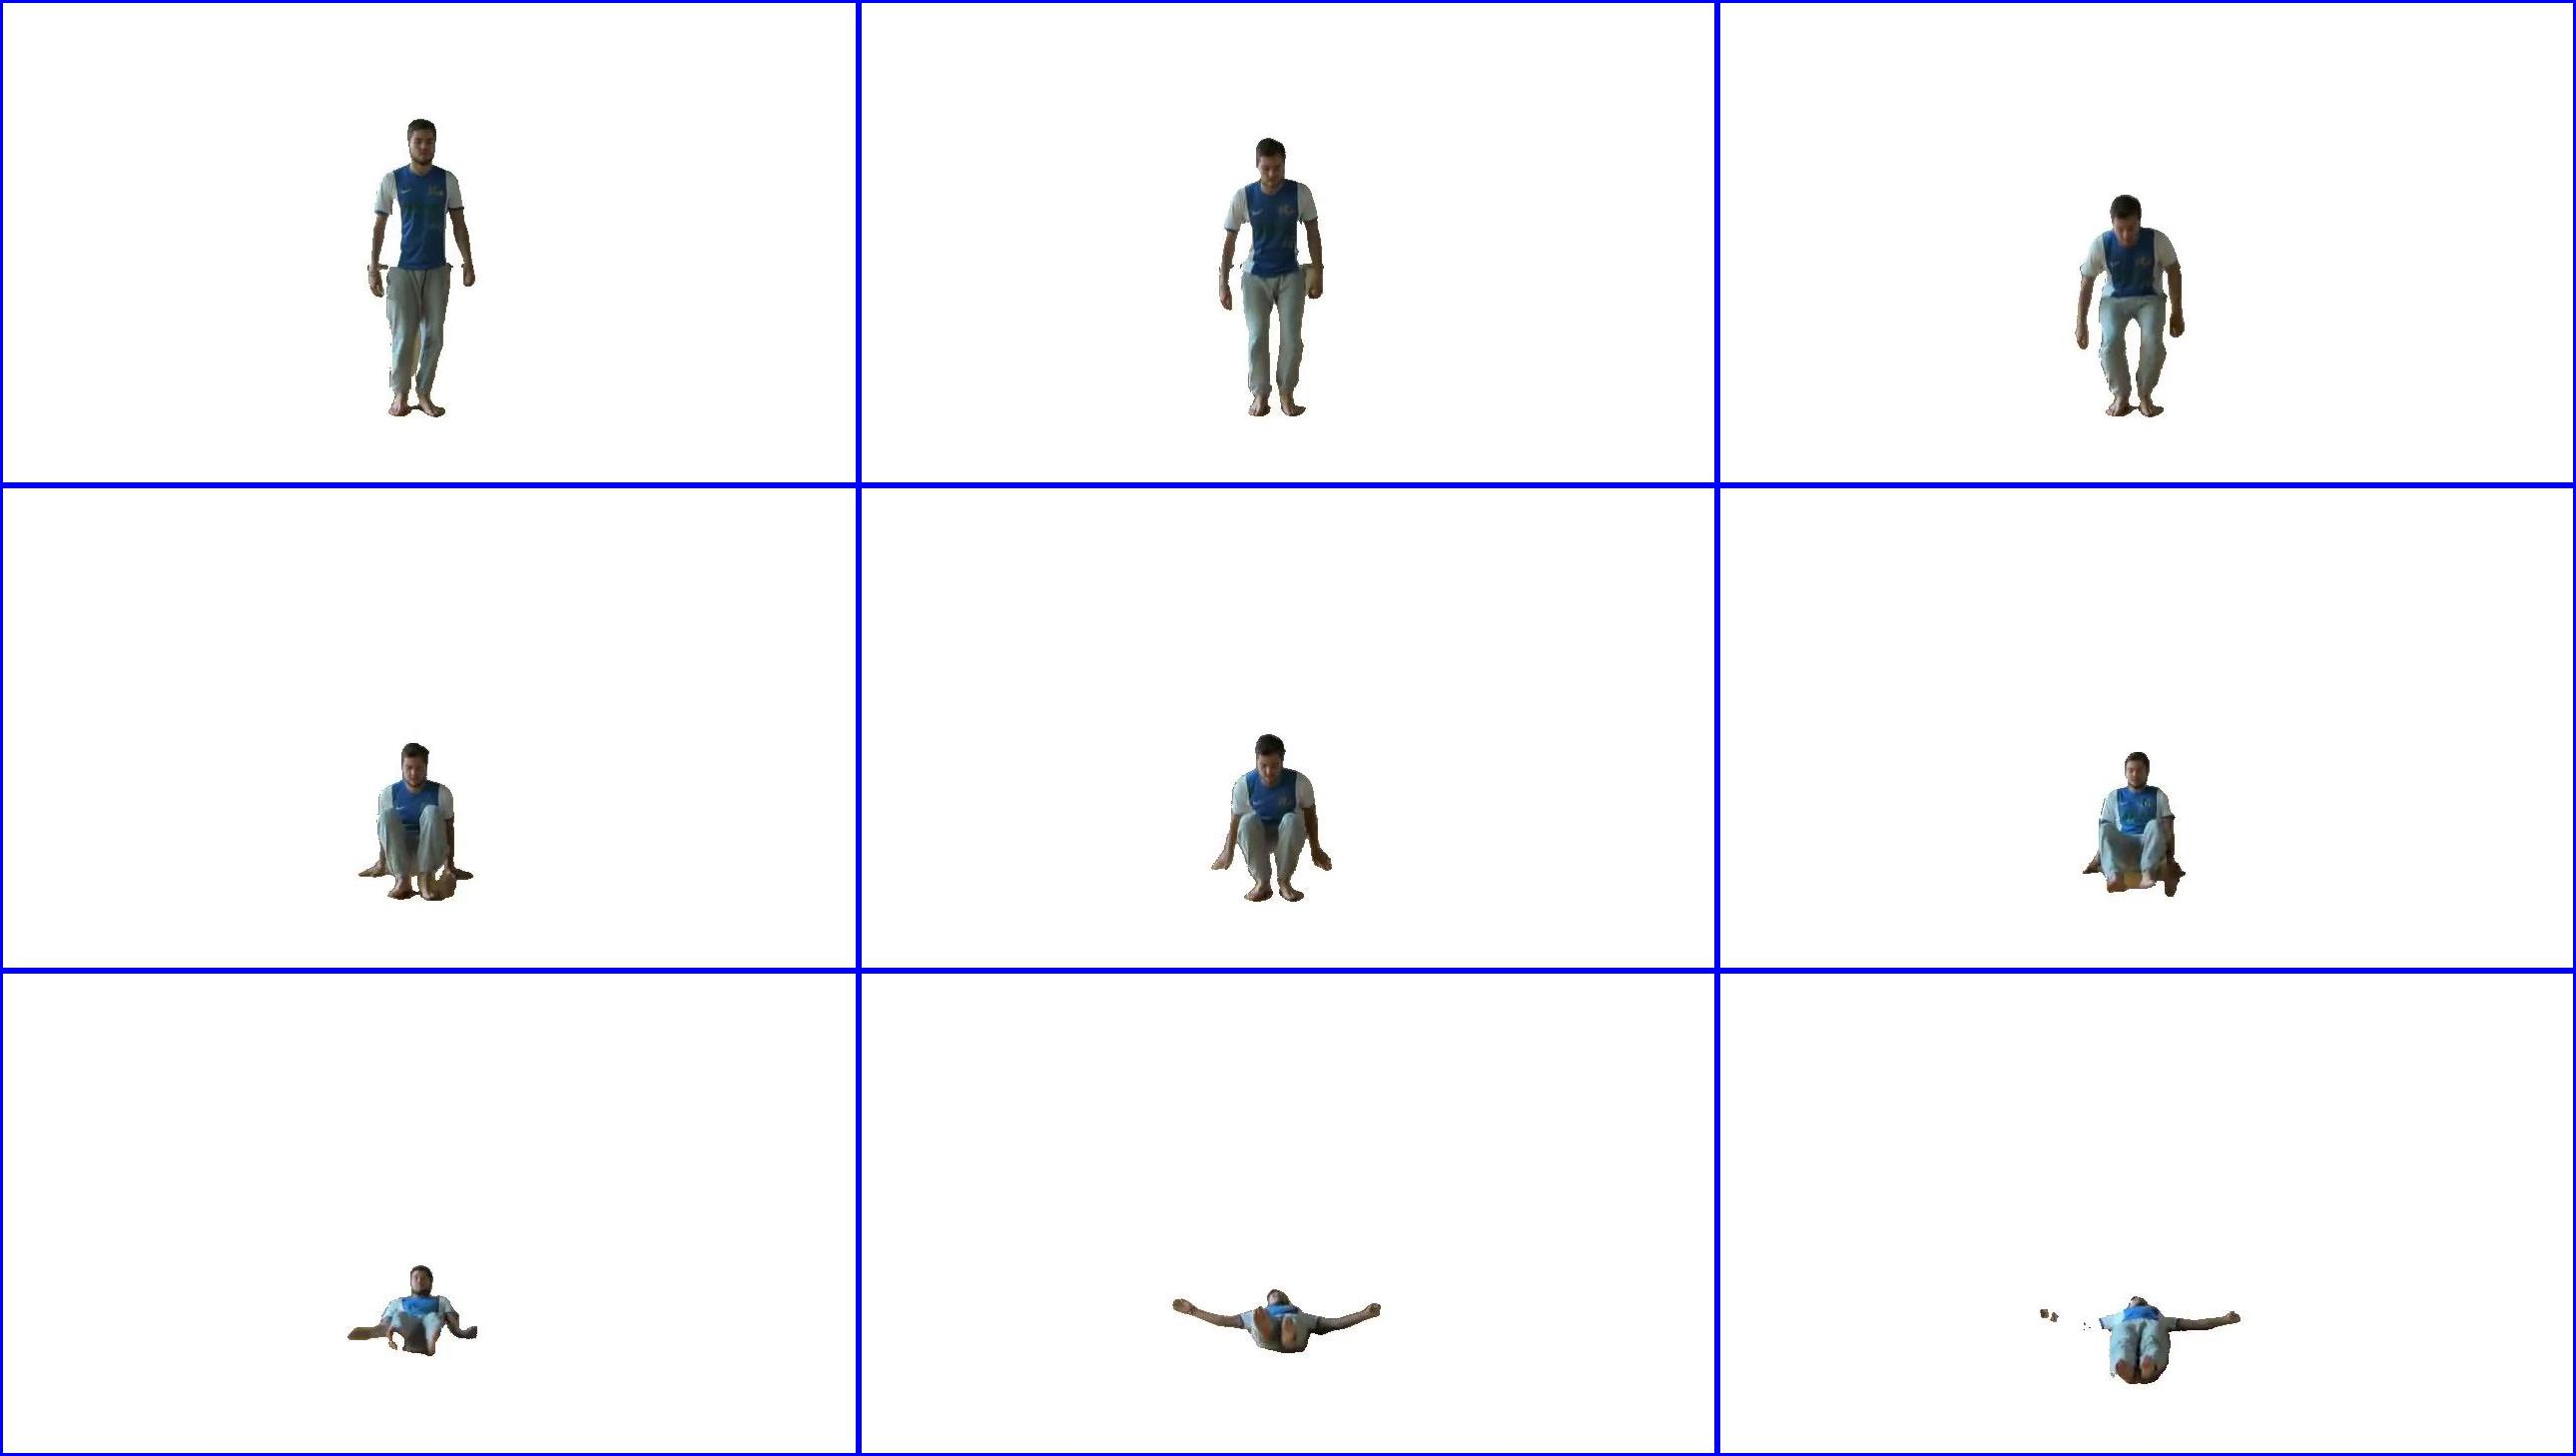
\includegraphics[height={230pt}, width={370pt}]{Thesis/images/fall_no_background.jpg}
\caption{Stripping the background through salient object detection for the \textit{fall} task}
\label{fig:fall_no_background}
\end{figure}

\begin{table}[h!]
  \begin{center}
    \caption{Experiments with background removal for the \textit{bast-base} task}
    \label{tab:research_question_5_no_background}
    \begin{tabular}{l|l|c|c|c}
      \textbf{Model} & \textbf{Background} & \textbf{Top2 Acc (test)} & \textbf{Top2 Acc (val)} & \textbf{Mean Class Acc}\\
      \hline
      \multirow{2}{*}{I3D} & \textit{original}& 96.3\% & 92.6\% & 87.1\%\\
      & \textit{blank-0.7d} & 20.4\% & 88.7\% & 15\%\\
      \hline
      \multirow{2}{*}{SlowOnly} & \textit{original}& 97.31\% & 95.1\% & 91.7\%\\
      & \textit{blank} & 26.8\% & 92.8\% & 17.3\%\\
      \hline
      \multirow{1}{*}{SlowOnly (no pre)} & \textit{blank} & 27.8\% & 90.1\% & 19.3\%\\
    \end{tabular}
  \end{center}
\end{table}

\bigskip
\noindent Table \ref{tab:research_question_5_no_background} shows the results for three experiments on two 3D models, namely \textit{I3D} with a \textit{kinetics} pre-training, \textit{SlowOnly} with a \textit{omni-sourced} pre-training, and finally \textit{SlowOnly} without pre-training. The results show that the models trained on a blank background have severely overfitted the dataset and are not able to generalize for unseen content. In the case of \textit{I3D} without background, the training was even done with a dropout rate of $0.7$, but that still did not help the final results. The validation accuracy of the models trained without a background is also lower when compared to models trained with one. The third experiment, namely training the \textit{SlowOnly} model from scratch, without any pre-training, also failed to generalize any better for unseen content, although the results were slightly better than the first two experiments, specifically, only $1\%$ better.

Figures \ref{fig:gradcam_no_background_model} and \ref{fig:gradcam_white_background_video} show the GradCAM results from the \textit{SlowOnly} model pre-trained on the \textit{omni-sourced} dataset. We can see that, even though we stripped the background, the blankness still plays a role in the model's predictions. This influence persists even when we run the model through a test video without background as shown in Figure \ref{fig:gradcam_white_background_video}, although this influence appears smaller than when feeding a video with a background as shown in Figure \ref{fig:gradcam_no_background_model}. When comparing Figure \ref{fig:gradcam_no_background_model} with Figure \ref{fig:GradCAM_slow_only}, we can see that the influence of the background is actually higher in the former, the model trained on videos without a background. In other words, models trained with a background perform better, and, moreover, the model is better able to pinpoint the user in the presence of a background than without one.

\bigskip
\noindent \textbf{Conclusion}: We conclude that stripping the background not only does not improve the model's performance but, on the contrary, it has an advert effect on it. The background is also essential for the model learning to pinpoint the human inside the frame as demonstrated by the above-presented GradCAM results. With the current state of research, it does not seem possible to produce models working with the \textit{RGB} modality that solely focus on human action. As was shown by the GradCAM results, even if the background is stripped, models are still influenced by it; that is, regardless of whether the background is neutral or not, it influences the model's final output. The following section briefly discusses skeleton models and how they solve the background influence problem. 
 
\begin{figure}[h]
\center
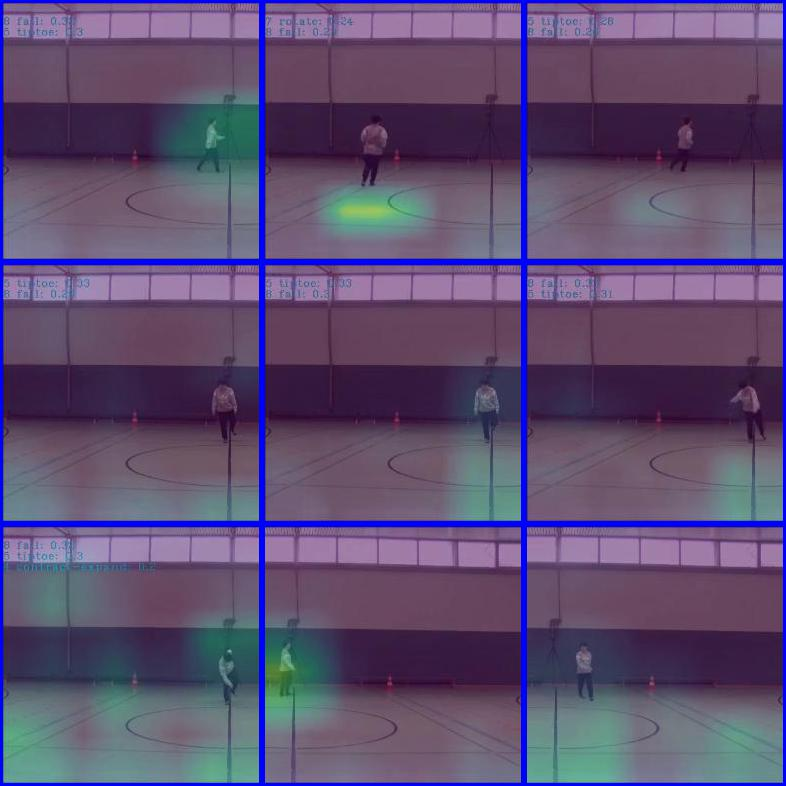
\includegraphics[height={250pt}, width={300pt}]{Thesis/images/gradcam_no_background.jpg}
\caption{GradCAM results on a SlowOnly model trained with videos without background but tested on a video with background}
\label{fig:gradcam_no_background_model}
\end{figure}

\begin{figure}[h]
\center
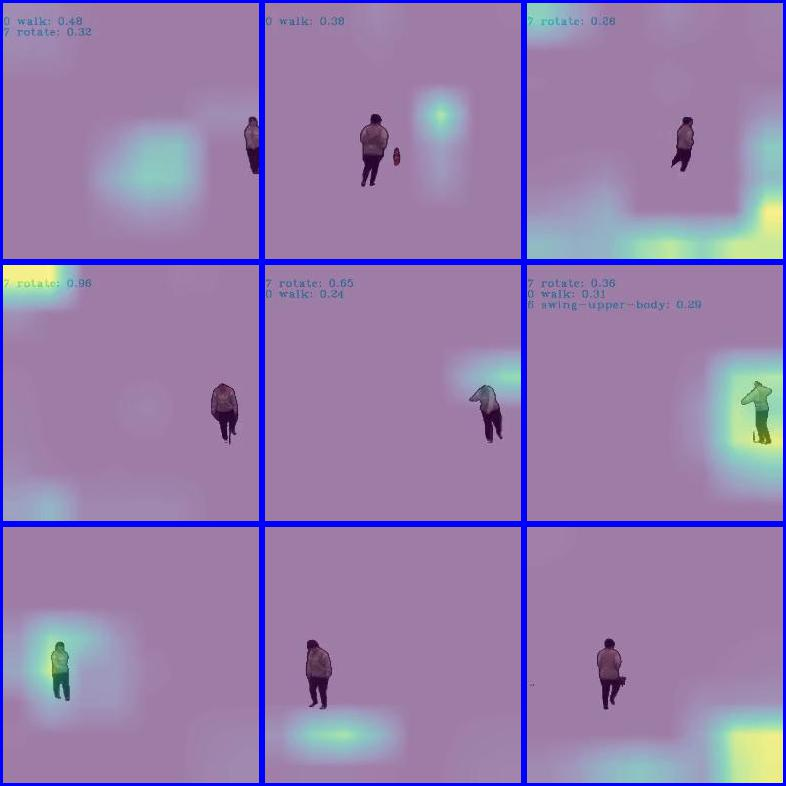
\includegraphics[height={250pt}, width={300pt}]{Thesis/images/gradcam_white_background.jpg}
\caption{GradCAM results on a SlowOnly model trained with videos without background and tested on a video without background}
\label{fig:gradcam_white_background_video}
\end{figure}

\subsubsection{Skeleton Models}
\label{research_question_5_4}
With the current state of research, the best input modality that could be used to avoid the background influence and differences in lightning variations would be to use skeleton-based models. As depicted in Figure \ref{walk_heatmap} and \ref{rotate_pose} these models can focus on the human skeleton in their entirely. The $17$ defined poses enable such models to be totally immune to contextual nuisances since they do not even take them into account.

\textit{RGB} and even \textit{optical-flow} based models, on the other hand, can be influenced by the background. This means that a prerequisite to training HAR models should be a diversification of such contextual conditions. In datasets used for this research, however, there was minimal background variance, and hence the use of skeleton-based models became even more crucial than otherwise would be the case. 


\newpage
\section{Threats and Conclusion}
\label{threats_and_conclusion}

\subsection{Threats}
\label{threats}
The main threat to most of the results that this thesis offers is the imbalanced and small datasets under disposal for the BAST domain itself but also the testing domains. Even though transfer learning ameliorated this problem significantly, it remains an open problem for models trained in this work. Indeed, in computer vision, we never can get enough data on the domain under inspection. Deep learning models, particularly 3D CNNs, are very prone to overfitting and underfitting, given the sheer sizes of their architectures. Therefore, the first prerequisite for future research in this topic should be having robust datasets.

\bigskip 
\noindent Robust datasets are also needed to validate the domain generalization capabilities of models trained on BAST materials. This thesis used the second part of the BAST dataset and a tiny dataset in the dancing domain for this purpose, and hence its results should only be taken as indicative and not as hard conclusions.

\subsection{Conclusion}
\label{conclusion}

This thesis focused on developing robust human action recognition 3D ConvNet models in the BAST domain. 2D ConvNet models were found to be under- and overfitting the tasks. Three different input modalities were used, namely skeleton data, RGB, and optical flow, the latter two also being combined with each other through late fusion. The purpose was to classify both the nine base annotations as well as the 42 evaluation annotations as the BAST analysis. For the former case, the classifiers were able to pinpoint the nine base actions with almost perfect accuracy, while on the latter, the best achieved \textit{top-3} accuracy was \textit{77.39\%}. This model could certainly be improved with a better dataset, and it was shown by examining the models' losses that this was possible.

\bigskip
\noindent In the context of the \textit{Vortanz} project, it was also examined, as far as it was feasible to do so, whether the two trained classifiers could be extended to other domains. For the nine base annotations, the experiment indicated that they could serve as general dancing categories in third domains. For the 42 evaluation annotations, the movements were found to be too specific to BAST and less prone to generalization to other domains. Moreover, it was concluded that it would be possible to automate the BAST evaluation analysis end-to-end, therefore removing the need to expert evaluators.

\bigskip
\noindent The next topic of study of this work was the benefits of transfer learning. It was shown that models trained on both tasks were able to procure significant improvements in their performance due to transfer learning of weights from other domains. It was found that the best benchmark datasets for the two BAST tasks were \textit{kinetics-400} and \textit{omni-sourced}. Finally, transfer learning using the \textit{bast-base} dataset itself on the \textit{bast-eval} task also proved indispensable to building robust models on the 42 annotations, and it was shown that this ameliorated the class-imbalance problem of this task to a certain extend.

\bigskip
\noindent The final avenue of research that this work pursued was the study of the background influence on the tasks at hand. It was shown that the background plays a big role towards the classifier's final prediction and that its influence cannot be suppressed without weakening the models themselves. Indeed, the experiment of stripping the background produced feeble models that were not able to generalize for unseen data. The best method to deaden the influence of the background on the models was found to be the use of a different input modality altogether, namely pose data, which solely focuses on the human action itself. Indeed, such models were the best performing models for both the \textit{bast-base} as well as the \textit{bast-eval} tasks.

\subsection{Future Work}
\label{future_work}

First of all, as already mentioned multiple times in the context of this work, a more extensive and more robust dataset would be needed to duly validate the main findings of this work duly. Also, it would be interesting to fuse the three input modalities, that is \textit{RGB}, \textit{Optical Flow}, and \textit{Pose} through late fusion and compare the performance as well as the complexity of such models with the ones tried in the context of this work. Finally, more tests should be conducted in various other domains to examine in more details how models trained on BAST material can generalize to these third contexts. 

\newpage
\bibliographystyle{alpha}
\bibliography{references.bib}
\end{document}


% gjashte nentor 2021